% $Id: msk-014-user.tex 9730 2021-12-21 20:25:11Z mskala $

%
% MSK 014 user/build manual
% Copyright (C) 2022  Matthew Skala
%
% This program is free software: you can redistribute it and/or modify
% it under the terms of the GNU General Public License as published by
% the Free Software Foundation, version 3.
%
% This program is distributed in the hope that it will be useful,
% but WITHOUT ANY WARRANTY; without even the implied warranty of
% MERCHANTABILITY or FITNESS FOR A PARTICULAR PURPOSE.  See the
% GNU General Public License for more details.
%
% You should have received a copy of the GNU General Public License
% along with this program.  If not, see <http://www.gnu.org/licenses/>.
%
% Matthew Skala
% https://northcoastsynthesis.com/
% mskala@northcoastsynthesis.com
%

\documentclass{ncmanual}

% \usepackage{bigstrut}
% \usepackage{dcolumn}
\usepackage{lilyglyphs}
\usepackage{musicography}
\usepackage{rotating}
\usepackage{stfloats}
\usepackage{tikz}

\usetikzlibrary{arrows.meta,calc,decorations,decorations.pathmorphing,patterns}

\newcommand{\blinkcodeLR}[4]{\begin{tikzpicture}[scale=0.6]
  \node at (-0.5,1) {L};
  \node at (-0.5,0) {R};
  \draw (0,-0.5) -- (0,1.5);
  \draw (8,-0.5) -- (8,1.5);
  \draw (0,0) -- (8,0);
  \draw (0,1) -- (8,1);
  \foreach \x/\y in {#1} {
    \draw[fill=green] (\x,0.65) rectangle (\y,1.35);
  }
  \foreach \x/\y in {#2} {
    \draw[fill=red] (\x,0.65) rectangle (\y,1.35);
  }
  \foreach \x/\y in {#3} {
    \draw[fill=green] (\x,-0.35) rectangle (\y,0.35);
  }
  \foreach \x/\y in {#4} {
    \draw[fill=red] (\x,-0.35) rectangle (\y,0.35);
  }
\end{tikzpicture}}

\newcommand{\blinkcodeX}[2]{\begin{tikzpicture}[scale=0.6]
  \node at (-0.71,0) {};
  \draw (0,-0.5) -- (0,0.5);
  \draw (8,-0.5) -- (8,0.5);
  \draw (0,0) -- (8,0);
  \foreach \x/\y in {#1} {
    \draw[fill=green] (\x,-0.35) rectangle (\y,0.35);
  }
  \foreach \x/\y in {#2} {
    \draw[fill=red] (\x,-0.35) rectangle (\y,0.35);
  }
\end{tikzpicture}}

\title{MSK~014\quad Gracious Host\\User/Build Manual}
\author{Matthew Skala}
\date{\today}

\begin{document}

\maketitle

%%%%%%%%%%%%%%%%%%%%%%%%%%%%%%%%%%%%%%%%%%%%%%%%%%%%%%%%%%%%%%%%%%%%%%%%

\begin{copyrightpage}
Hardware documentation for the MSK~014\\
Copyright \copyright\ 2022 Matthew Skala

\GPLThreeStatement
\end{copyrightpage}

\tableofcontents

%%%%%%%%%%%%%%%%%%%%%%%%%%%%%%%%%%%%%%%%%%%%%%%%%%%%%%%%%%%%%%%%%%%%%%%%

\texdependspdfworkaround

% $Id: general.tex 9828 2022-02-10 17:51:13Z mskala $

%
% MSK 014 general notes
% Copyright (C) 2022  Matthew Skala
%
% This program is free software: you can redistribute it and/or modify
% it under the terms of the GNU General Public License as published by
% the Free Software Foundation, version 3.
%
% This program is distributed in the hope that it will be useful,
% but WITHOUT ANY WARRANTY; without even the implied warranty of
% MERCHANTABILITY or FITNESS FOR A PARTICULAR PURPOSE.  See the
% GNU General Public License for more details.
%
% You should have received a copy of the GNU General Public License
% along with this program.  If not, see <http://www.gnu.org/licenses/>.
%
% Matthew Skala
% https://northcoastsynthesis.com/
% mskala@northcoastsynthesis.com
%

\chapter{General notes}

This manual documents the MSK~014 Gracious Host, which is a module for use
in a Eurorack modular synthesizer.  The module's main function is provide an
interface from USB devices, especially MIDI controllers, to the CV/gate
synthesizer.  As the name implies, the Gracious Host functions as an
embedded host, capable of connecting devices like keyboards without
needing the involvement of a separate computer.  It supports multiple
control modes for use in different kinds of patches, and the onboard
microcontroller can be reprogrammed in the field with new or modified
firmware loaded from a USB flash drive through the front-panel port.

This is one of two manuals.  The other manual is specifically intended for
programmers who are modifying or replacing the firmware, and is of less
interest for most users.

\section{Front panel connections}

The front panel of the Gracious Host is shown in
Figure~\ref{fig:panel-mockup}.  The fragment of music notation on the panel
spells GRACE as a pun on the module name:  treble clef (G clef); quarter-note
rest (R); and the three notes A, C, E.

\begin{figure*}
{\centering\setlength{\fboxsep}{0pt}\setlength{\fboxrule}{0.6pt}%
 \fbox{\includegraphics{panel-mockup.pdf}}\par}
\caption{Module front panel.}\label{fig:panel-mockup}
\end{figure*}

\subsection{Serial bus port}

The port at upper left is for connecting a USB device, such as a USB-MIDI
keyboard.  This is an \emph{embedded host} port, capable of supporting many
USB 1.0, 1.1, and 2.0 low-speed and full-speed devices relevant to
synthesizer use, but it does not support the entire USB standard with every
configuration of every device.  Exactly what the module will do depends on
what kind of device is plugged in; it will normally detect whenever a device
is inserted or removed, and go into a mode appropriate for that device, with
the different modes described in subsequent chapters of this manual.

The port is intended only for standard low-power devices such as MIDI
controllers.  The maximum current it is \emph{intended} to support is
100\,mA (which is a ``unit load'' according to the relevant USB
standards).  Some devices may attempt to draw more, and may succeed, but this
port is not intended for high-power applications like battery charging.

The Gracious Host cannot make use of a hub.  The USB device must be
attached directly to the port, and only one USB device can be attached at a
time.

\subsection{Control voltage inputs}

The top pair of jacks, labelled ``IN,'' serve as control voltage inputs,
which may be gate/trigger or pitch control voltages depending on the
operating mode.  Although the module will not be damaged by voltages between
the power supply rails ($\pm$12V when the module is powered up), the useful
range of voltages over which the analog-to-digital converters can work
properly is from 0V to $+$5V.

The nominal input impedance for these jacks is 100k$\Omega$.

\subsection{Bi-colour LEDs}

Immediately below the input jacks is a pair of bi-colour (red and green)
LEDs.  These display status information with a function that depends on the
operating mode.  For instance, in most MIDI-controller modes, the LED on one
side of the module will light when that side is playing a note.

\subsection{Control voltage (analog) outputs}

The second pair of jacks from the top, labelled ``CV,'' are multi-purpose
analog control voltage outputs with an intended operating range of 0V to
$+$5V.  These are typically used for things like pitch and velocity, again
depending on the mode.  In a few modes where these jacks are used for
trigger or gate output, they may produce a slightly higher uncalibrated
voltage like $+$5.5V.

\subsection{Gate (digital) outputs}

The bottom pair of jacks, labelled ``GT,'' produce digital control voltages
(gates or triggers), with ``low'' at 0V to within the tolerances of op amp
offsets, and ``high'' at approximately 9V.

\section{Specifications}

The nominal impedance for the input jacks is 100k$\Omega$.  All the outputs
are driven by op amps with in-the-loop 1k$\Omega$ resistors, giving them
effectively zero output impedance in normal use but limiting the output
current to about 10\,mA under short-circuit conditions.

Briefly shorting any input or output to any fixed voltage at or between the
power rails, or shorting two to each other, should be harmless to the
module.  Note that ``between the power rails'' does mean it is safer to feed
voltages into the module when power is applied, since without power, both
power rails will be at zero.  Patching the MSK~014's output into the output
of another module should be harmless to the MSK~014, but doing that is not
recommended because it is possible the other module may be harmed.

This module contains series reverse protection diodes and is unlikely to be
damaged by a reverse power connection, but because it uses a 16-pin power
connection, there are more kinds of misconnection possible than pure reversal
of the main power rails.  It is possible that there could be a short
circuit, more likely damaging to the power supply than to the module, if the
power is misconnected.  The connector on the module is polarized and
unlikely to be misconnected, but some caution is still recommended when
connecting the cable at the bus board.

The maximum current demand of this module in normal operation is 10\,mA from
the $+$12V supply, 20\,mA from the $-$12V supply, and a variable amount from
the $+$5V supply.  For power budgeting purposes I suggest counting the
Gracious Host's $+$5V requirement as 130\,mA, though the details are more
complicated, as described below.  Placing an unusually heavy load on the
outputs (for instance, with so-called passive modules, output-to-output
patching, or attempting to charge USB devices from the front-panel port) can
increase the power supply current beyond these levels.

In more detail:  the Gracious Host supplies $+$5V power more or less
directly from the Eurorack bus to the attached USB device, so the amount
drawn from the Eurorack bus will depend on what is attached to the
front-panel USB port.  The Gracious Host needs up to 30\,mA of $+$5V itself,
plus whatever is drawn by the USB device.  USB devices, according to the
relevant specifications, are supposed to draw at most 100\,mA and then
request more from the host if desired -- but the standard Gracious Host
firmware will never give the device permission to draw extra power.  Thus in
normal operation with standards-compliant devices, 130\,mA should be the
maximum consumption of $+$5V Eurorack power for the module and the attached
device.

Now, on the one hand, nearly all devices commonly expected to be used with
the Gracious Host will actually consume much less than 100\,mA; 5--20\,mA is
more typically expected, and so in actual practice the maximum total $+$5V
consumption is likely to be 35--50\,mA.  However, some high-power USB
devices actually draw more than the specified 100\,mA maximum without
following the protocol for requesting it.  The Gracious Host uses a PTC
thermistor, often called a thermal fuse although it really is not a fuse at
all, to protect against short circuits.  This protective device has a
\emph{hold current} of 200\,mA (meaning that at that level it will
not trip) and a \emph{trip current} of 400\,mA (meaning that at that level
it will trip in a few seconds).  So, if somewhat overloaded, the module
could consume as much as 230\,mA of Eurorack $+$5V power continuously; and
if heavily overloaded it could briefly draw much more before the thermal
fuse trips.

\section{Modification:  onboard $+$5V regulator}

\emph{The Gracious Host requires $+$5V power, up to 130\,mA under ordinary
recommended use.}

In the standard configuration, this module requires a power supply that
offers $+$5V.  It will not work if plugged into a stripped-down Eurorack
power supply with only $\pm$12V.  The decision was made to require
$+$5V because at present nearly all commercial Eurorack power supplies do in
fact offer $+$5V; the Gracious Host and the attached USB device each require
a significant amount of current, with the typically spiky demand of digital
circuitry; and attempting to convert $\pm$12V to $+$5V on board the module
would raise significant thermal, noise, and other technical issues, all just
to serve the small minority of users who have no $+$5V supply already.

However, for special purposes such as bench-top testing, it is possible to
solder in a 7805 regulator chip, on the pads next to the protection diodes,
as shown.  Photo depicts an early prototype with green solder mask instead
of production blue, and some minor differences in other details.  Then by
changing the configuration jumper settings (next section), the module can be
configured to draw its $+$5V current from the $+$12V instead, through the
installed regulator, with no requirement for an external $+$5V supply.

\nopagebreak\noindent
{\hspace*{\fill}\includegraphics[width=\linewidth]{optional-7805.jpg}\hspace*{\fill}\par} 

The 7805 regulator chip is not included in kits, and adding it is not a
recommended or supported configuration.  Depending on the amount of current
drawn by the external USB device, a 7805 installed as shown without a heat
sink may be liable to overheat.  Using an external device that needs maximum
rated power, or more, for more than a few seconds at a time may necessitate
adding a heat sink to the 7805 chip.  Furthermore, it is possible to set the
configuration jumpers in such a way that the on-board 7805 will be
cross-connected with the Eurorack bus -- meaning that it will attempt to
supply $+$5V power to other modules (possibly useful, but further increasing
the likelihood of overheating), or interfere with the existing bus $+$5V
supply if there is one after all.

The 7805, if installed, will have very little effect unless also activated
with the ``R'' jumper described below, so it remains possible to use a
modified module with bus power instead as long as you are careful with the
jumper configuration.

\section{Bus access and configuration jumpers}

There is a jumper block on the back of the module for selecting the $+$5V
source and whether to connect the first channel (left side of the front
panel) output jacks to the Eurorack bus.
\emph{At least one jumper (the one selecting $+$5V source) must be correctly
installed for the Gracious Host to operate at all.}

\nopagebreak\noindent
{\hspace*{\fill}\includegraphics[width=\linewidth]{jumpers.jpg}\hspace*{\fill}\par} 

Left to right, the jumper positions are:
\begin{itemize}
  \item ``G'':  install to connect left GT output to the ``gate'' bus;
  \item ``C'':  install to connect left CV output to the ``pitch CV'' bus;
  \item ``5'':  install to draw $+$5V power from the Eurorack bus;
  \item ``X'':  spare position, no effect; and
  \item ``R'':  install to draw $+$5V power from the onboard regulator, if
    one is installed -- otherwise no effect.
\end{itemize}

Four pins of the standard Eurorack bus are reserved for transmitting pitch
and gate CV among modules.  Most Eurorack cases will connect these pins
among modules -- usually with a separate CV/gate bus for each busboard in
multi-busboard systems.  Some of Doepfer's VCOs, like the A-110-1, receive
pitch CV from the bus by default when no pitch CV is connected to the front
panel, and North Coast's Middle Path VCO (the MSK~013) does the same. 
Modules like the Doepfer A-185-2 are capable of transmitting CV and gate
signals onto the bus.  Some Cwejman, Macbeth, MakeNoise, Malekko, MFB, Plan
B, Synthwerks, TipTop, and other manufacturers' modules also use these pins
in a compatible way.  So with compatible VCOs, you can just plug the
Gracious Host into the same busboard and have it control the VCO pitch
without needing to patch them with front-panel cables.  Similarly, you may
be able to have the gate signal from the Gracious Host activate envelopes or
VCAs without patching.

Some manufacturers have attempted to send digital signals over the CV/gate
bus in a non-standard way under the name ``sync bus.'' Despite more than one
using this name, each manufacturer attempting digital use of the bus has
defined its own nonstandard format for the signals (usually some variation
of MIDI adapted to voltage levels instead of current-loop), and they are not
in general compatible with each other.  Such use also is not compatible with
the analog use of the CV/gate bus as defined by Doepfer, and the two should
not be mixed.

To have the Gracious Host transmit pitch and gate CV onto the bus, install
jumpers in the first two positions, labelled ``G'' and ``C.'' These two
jumpers have the effect of connecting the output jacks directly to the bus. 
It is also possible to install just one of the two jumpers, to transmit only
pitch or only gate CV.  The standard or default configuration for assembled
modules sold by North Coast Synthesis is to install both these jumpers; but
it \emph{will} be necessary to remove them for good results if using more
than one Gracious Host on the same bus.  At most one module on a given
Eurorack bus should be configured to drive the CV/gate bus.  Setting up more
than one module as the bus master is equivalent to patching their outputs
into each other, and is unlikely to work well.

Install a jumper at the third position, labelled ``5,'' to connect the
Gracious Host's internal $+$5V supply to the Eurorack bus.  This should
always be done, for standard unmodified Gracious Host modules.  The only
reason not to install this jumper would be if the module has been modified
with an onboard regulator, in which case you could install the jumper in the
fifth position (``R'') instead, to use the installed onboard regulator.  It
would also be possible to install jumpers at both positions ``5'' and ``R,''
in which case the modified Gracious Host will attempt to regulate $+$12V
power down to $+$5V \emph{and also} supply that power to other modules
through the bus.  Doing so is potentially dangerous, but could possibly be
useful in a very small system where it might be desired to support some
other $+$5V module when the main power supply has no $+$5V rail.

The fourth jumper position (``X'') is unconnected, and the fifth (``R'')
is also unconnected in a standard build.  So, in an unmodified module, these
two jumper positions may be used as storage locations for the two extra
jumpers when CV/gate bus access is \emph{not} desired.  That way, there is
less risk of losing the jumpers.

\section{Source package}

A ZIP archive containing source code for this document and for the module
itself, including things like machine-readable CAD files, is available from 
the Web site at 
\url{https://northcoastsynthesis.com/}.  Be aware that actually building
from source requires some manual steps; Makefiles for GNU Make are provided,
but you may need to manually generate PDFs from the CAD files for inclusion
in the document, make Gerbers from the PCB design, manually edit the .csv
bill of materials files if you change the bill of materials, and so on.

Recommended software for use with the documentation and hardware source code
includes:
\begin{itemize}
  \item GNU Make;
  \item \LaTeX\ for document compilation;
  \item LaTeX.mk (Danjean and Legrand, not to be confused with other
    similarly-named \LaTeX-automation tools);
  \item Circuit\_macros (for in-document schematic diagrams);
  \item Kicad (electronic design automation);
  \item Qcad (2D drafting); and
  \item Perl (for the BOM-generating script).
\end{itemize}

The kicad-symbols/ subdirectory contains my customised schematic symbol and
PCB footprint libraries for Kicad.  Kicad doesn't normally keep dependencies
like symbols inside a project directory, so on my system, these files
actually live in a central directory shared by many projects.  As a result,
upon unpacking the ZIP file you may need to do some reconfiguration of the
library paths stored inside the project files, in order to allow the symbols
and footprints to be found.  Also, this directory will probably contain some
extra bonus symbols and footprints not actually used by this project,
because it's a copy of the directory shared with other projects.

The source package also contains source code for the module firmware, which
is written in PIC24 assembly language and documented in the \emph{MSK~014
Gracious Host Programmer's Manual}.  Working with that code will require
additional software tools -- in particular, Microchip's version of the GNU
assembly language toolchain.

The whole package is covered by the GNU GPL, version 3, a copy of which is
included in the file COPYING.

\section{PCBs and physical design}

The enclosed PCB design is for two boards, each
3.90$''$\linebreak[0]$\times$\linebreak[0]1.50$''$ or
99.06mm\linebreak[0]$\times$\linebreak[0]38.10mm.
The two boards are intended to
mount in a stack parallel to the Eurorack panel, held together with M3
machine screws and male-female hex standoff hardware.  See
Figure~\ref{fig:panel-stack}.  With 12mm of clearance for the power
connector and cable, the module should fit in about 39mm of depth measured from the
back of the front panel.

\begin{figure}
{\centering
\begin{tikzpicture}[scale=0.1]
  % power connector clearance
  \path[draw=black,dashed,thick] (27.2,-54.00) rectangle (39.2,-35.59);
  % panel
  \path[draw=black,fill=black!30!white] (-2.0,-64.25) rectangle (0,64.25);
  % panel-board 1 standoffs
  \path[draw=black,fill=white] (0,-32.93) rectangle (13,-26.93);
  \path[draw=black,fill=white] (0,51.72) rectangle (13,45.72);
  % board 1
  \path[draw=black,fill=blue!50!white] (13,-46.53) rectangle (14.6,52.53);
  % board 1-board 2 standoffs
  \path[draw=black,fill=white] (14.6,-32.93) rectangle (25.6,-26.93);
  \path[draw=black,fill=white] (14.6,51.72) rectangle (25.6,45.72);
  % board 2
  \path[draw=black,fill=blue!50!white] (25.6,-46.53) rectangle (27.2,52.53);
  % nuts and standoff thread ends at back
  \path[draw=black,fill=white] (27.2,-32.93) rectangle (29.2,-26.93);
  \path[draw=black,fill=white] (27.2,51.72) rectangle (29.2,45.72);
  \path[draw=black,fill=black!10!white] (29.2,-30.93) rectangle (31.2,-28.93);
  \path[draw=black,fill=black!10!white] (29.2,49.72) rectangle (31.2,47.72);
  % labels, arrows
  \node at (6.5,38) {\parbox{10mm}{\centering \small 13mm standoff}};
  \node at (20.1,38) {\parbox{11mm}{\centering \small 11mm standoff}};
  \node at (13,64) {\small 2mm front panel};
  \node at (21.4,60.5) {\small 2$\times$ 1.6mm PCBs};
  \draw[>=latex',->,very thick] (13.8,58.7) -- (13.8,53.0);
  \draw[>=latex',->,very thick] (26.4,58.7) -- (26.4,53.0);
  \node at (36.2,-18)
    {\parbox{17mm}{\centering \small 12mm clearance for mated power connector}};
  \draw (39.2,-55) -- (39.2,-64);
  \draw[>=latex',<->,thick] (0,-59.5) -- (39.2,-59.5);
  \node[fill=white] at (20.0,-59.5) {\small $\approx$39mm depth};
\end{tikzpicture}\par}
\caption{Assembled module, side view.}\label{fig:panel-stack}
\end{figure}

\section{Blink codes}

The two bi-colour LEDs on the front panel are used for multiple purposes. 
In most modes they light up in time with the notes being played.  They
flicker briefly when a USB device is inserted, both as a generic indicator
that something is happening, and to support debugging of the stages of the
USB attachment process.  But in some special situations the LEDs display
coded blinking patterns that report the module's status or error condition,
and these patterns are illustrated in this manual with diagrams like the
ones below.  Time reads left to right, with the entire diagram representing
a cycle that repeats every 1.05s.

If a hub is inserted in the USB port -- bearing in mind that the Gracious
Host does not work with hubs -- it will display bursts of four short red
flashes (Morse code ``H'' for ``hub'') on the right LED, leaving the left
LED dark, until the hub is removed.

\nopagebreak
\blinkcodeLR{}{}{}{0/0.5,1/1.5,2/2.5,3/3.5}

For an unsupported device other than a hub, the blink code is similar to the
one for ``hub,'' but the flashes are in a long-short-short pattern; Morse
code ``D'' for ``device unsupported.''

\nopagebreak
\blinkcodeLR{}{}{}{0/1.5,2/2.5,3/3.5}

In the event that something goes wrong inside a per-device USB driver and
the module is unable to recover while the device is attached, it displays
very fast back-and-forth red flashes until the device is removed.

\nopagebreak
\blinkcodeLR{}{0/0.5,1/1.5,2/2.5,3/3.5,4/4.5,5/5.5,6/6.5,7/7.5}%
{}{0.5/1,1.5/2,2.5/3,3.5/4,4.5/5,5.5/6,6.5/7,7.5/8}

If the module gracefully detects a trip of the USB polyfuse, indicating a
short circuit or that someone tried to charge a non-compliant high-power
device through the USB port, then in principle the firmware will try to
display a pattern of mostly red interrupted by short green flashes and
pauses.  Really, though, this display is unlikely to work; in actual testing
of an overloaded port condition the module is often sufficiently messed up
that it shuts off until power-cycled, or at least until the polyfuse cools
down.

\nopagebreak
\blinkcodeLR{3/3.5,5.5/6}{1/3,3.5/5.5,6/8}%
{1.5/2,7/7.5}{0/1.5,2/4,5/7,7.5/8}

There are other blink codes specific to the calibration procedure, which are
illustrated in the section on calibration.

\section{Use and contact information}

This module design is released under the GNU GPL, version 3, a copy of which
is in the source code package in the file named \texttt{COPYING}.  One
important consequence of the license is that if you distribute the design to
others -- for instance, as a built hardware device -- then you are obligated
to make the source code available to them at no additional charge, including
any modifications you may have made to the original design.  Source code for
a hardware device includes without limitation such things as the
machine-readable, human-editable CAD files for the circuit boards and
panels.  You also are not permitted to limit others' freedoms to
redistribute the design and make further modifications of their own.

I sell this and other modules, both as fully assembled products and
do-it-yourself kits, from my Web storefront at
\url{http://northcoastsynthesis.com/}.  Your support of my business is what
makes it possible for me to continue releasing module designs for free. 
The latest version of this document and the associated source files can be
found at that Web site.

Email should be sent to\\ \url{mskala@northcoastsynthesis.com}.

% $Id: nonusb.tex 9713 2021-12-18 19:22:35Z mskala $

%
% Non-USB operation
% Copyright (C) 2022  Matthew Skala
%
% This program is free software: you can redistribute it and/or modify
% it under the terms of the GNU General Public License as published by
% the Free Software Foundation, version 3.
%
% This program is distributed in the hope that it will be useful,
% but WITHOUT ANY WARRANTY; without even the implied warranty of
% MERCHANTABILITY or FITNESS FOR A PARTICULAR PURPOSE.  See the
% GNU General Public License for more details.
%
% You should have received a copy of the GNU General Public License
% along with this program.  If not, see <http://www.gnu.org/licenses/>.
%
% Matthew Skala
% https://northcoastsynthesis.com/
% mskala@northcoastsynthesis.com
%

\chapter{Non-USB operation}

\begin{figure*}[b]
{\centering
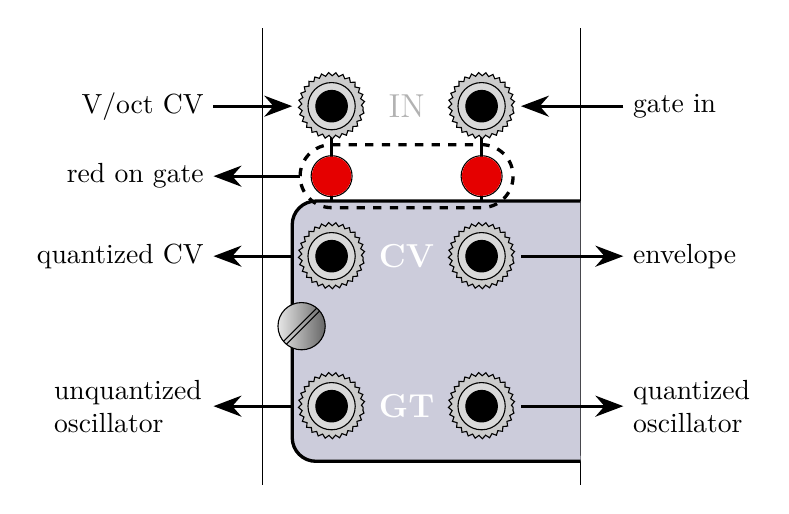
\begin{tikzpicture}
  {\setmainfont[Path={../../tsukurimashou/otf/},
BoldFont={TsukurimashouBokukkoExtraBoldPS}]{TsukurimashouBokukkoDemiboldPS}%
% start out defining coordinates
\coordinate (lbh) at (4.91mm,31.23mm) {};
\coordinate (j1) at (8.72mm,59.17mm) {};
\coordinate (j2) at (27.77mm,59.17mm) {};
\coordinate (j3) at (8.72mm,40.12mm) {};
\coordinate (j4) at (27.77mm,40.12mm) {};
\coordinate (j5) at (8.72mm,21.07mm) {};
\coordinate (j6) at (27.77mm,21.07mm) {};
\coordinate (d5) at (8.72mm,50.28mm) {};
\coordinate (d6) at (27.77mm,50.28mm) {};
%
\draw (0,11.07mm) -- (0,69.07mm);
\draw (40.30mm,11.07mm) -- (40.30mm,69.07mm);
%
\draw[very thick,black] (j1) -- (j3);
\draw[very thick,black] (j2) -- (j4);
\draw[very thick,black,fill=blue!30!black!20!white,rounded corners=3.0mm]
  (40.30mm,47.12mm) -- (3.72mm,47.12mm) --
  (3.72mm,14.07mm) -- (40.33mm,14.07mm);
\node[black!30!white] at ($(j1)!0.5!(j2)$) {\large IN};
\node[white] at ($(j3)!0.5!(j4)$) {\large\textbf{CV}};
\node[white] at ($(j5)!0.5!(j6)$) {\large\textbf{GT}};
%
% board-to-panel mounting holes, to clear M3 machine screw
\draw (lbh) circle[radius=1.60mm];
% six jacks with M6 threads, 6.3mm holes
\draw (j1) circle[radius=3.15mm];
\draw (j2) circle[radius=3.15mm];
\draw (j3) circle[radius=3.15mm];
\draw (j4) circle[radius=3.15mm];
\draw (j5) circle[radius=3.15mm];
\draw (j6) circle[radius=3.15mm];
% two LEDs, 5.20mm holes
\draw (d5) circle[radius=2.60mm];
\draw (d6) circle[radius=2.60mm];
%
% mock up screw heads, knobs
% machine screws with 6mm heads
\foreach \screwname in {lbh} {
  \path[draw=black,shading=ball,
    left color=black!10!white,right color=black!60!white]
    (\screwname) circle[radius=3mm];
  \draw ($(\screwname)+(50:3.0mm)$)--($(\screwname)+(220:3.0mm)$);
  \draw ($(\screwname)+(40:3.0mm)$)--($(\screwname)+(230:3.0mm)$);
}
% jacks with knurled nuts
\foreach \jackname in {j1,j2,j3,j4,j5,j6} {
  \path[draw=black,fill=black!20!white,
    decorate,decoration={snake,amplitude=0.6,segment length=2.5}]
    ($(\jackname)+(0,-0.15mm)$) circle[radius=4mm];
  \path[draw=black,fill=black!15!white] (\jackname) circle[radius=3mm];
  \path[draw=black,fill=black] (\jackname) circle[radius=2mm];
}
}

%
  \path[fill=red!90!black] (d5) circle[radius=2.50mm];
  \path[fill=red!90!black] (d6) circle[radius=2.50mm];
  \draw[very thick,-{Stealth[scale=1.2]}]
    ($(j1)+(-15mm,0)$) -- ($(j1)+(-5mm,0)$);
  \draw[very thick,-{Stealth[scale=1.2]}]
    ($(j2)+(18mm,0)$) -- ($(j2)+(5mm,0)$);
  \draw[very thick,{Stealth[scale=1.2]}-]
    ($(d5)+(-15mm,0)$) -- ($(d5)+(-4mm,0)$);
%  \draw[very thick,{Stealth[scale=1.2]}-]
%    ($(d6)+(18mm,0)$) -- ($(d6)+(4mm,0)$);
  \draw[rounded corners=4mm,very thick,dashed]
    ($(d5)+(-4mm,-4mm)$) rectangle ($(d6)+(4mm,4mm)$);
  \draw[very thick,{Stealth[scale=1.2]}-]
    ($(j3)+(-15mm,0)$) -- ($(j3)+(-5mm,0)$);
  \draw[very thick,{Stealth[scale=1.2]}-]
    ($(j4)+(18mm,0)$) -- ($(j4)+(5mm,0)$);
  \draw[very thick,{Stealth[scale=1.2]}-]
    ($(j5)+(-15mm,0)$) -- ($(j5)+(-5mm,0)$);
  \draw[very thick,{Stealth[scale=1.2]}-]
    ($(j6)+(18mm,0)$) -- ($(j6)+(5mm,0)$);
%
  \node[anchor=east] at ($(j1)+(-15mm,0)$) {V/oct CV};
  \node[anchor=west] at ($(j2)+(18mm,0)$) {gate in};
  \node[anchor=east] at ($(d5)+(-15mm,0)$) {red on gate};
  \node[anchor=east] at ($(j3)+(-15mm,0)$) {quantized CV};
  \node[anchor=west] at ($(j4)+(18mm,0)$) {envelope};
  \node[anchor=east] at ($(j5)+(-15mm,0)$)
    {\parbox{19mm}{unquantized oscillator}};
  \node[anchor=west] at ($(j6)+(18mm,0)$)
    {\parbox{15mm}{quantized oscillator}};
\end{tikzpicture}\par}
\caption{Jack/LED functions for non-USB mode.}\label{fig:non-usb-jacks}
\end{figure*}

The Gracious Host is meant to work with a USB device like a MIDI controller,
but as a default, with no USB device connected, the standard firmware will
function as a baby synth voice.  See Figure~\ref{fig:non-usb-jacks} for the
panel jack assignments in this mode.

The left CV input is volt per octave pitch, with a nominal range from 0V for
MIDI note 36 (C two octaves below Middle C, 65.406Hz) to 5V for MIDI note
96 (C three octaves above Middle C, 2093.004Hz).  The right CV input is for
a gate signal (threshold approximately 1.62V).  Both LEDs will light, in red,
when the gate is high.

The left CV output is a semitone quantized version of the CV input.  The
right CV output is an ADSR envelope with fixed parameters.  And the two
digital outputs are square wave oscillators:  unquantized pitch on the left,
quantized pitch on the right.

\newpage

The unquantized oscillator runs only while
the gate is high, whereas the quantized oscillator runs continuously once
started.  The concept here is that you could use the module with an external
VCA and the quantized and envelope outputs to get sound during the decay tail, or just
use the unquantized output directly and have a very basic synth voice in the
Gracious Host alone.

Note that the digital outputs, as usual, produce only the fixed levels of 0V
for low and approximately 9V for high; so the square waves on these outputs
include a DC offset of approximately 4.5V.

If you connect a USB device, the module will leave this mode and attempt to
do something appropriate to the device instead.

% $Id: midi.tex 9713 2021-12-18 19:22:35Z mskala $

%
% MIDI interface
% Copyright (C) 2022  Matthew Skala
%
% This program is free software: you can redistribute it and/or modify
% it under the terms of the GNU General Public License as published by
% the Free Software Foundation, version 3.
%
% This program is distributed in the hope that it will be useful,
% but WITHOUT ANY WARRANTY; without even the implied warranty of
% MERCHANTABILITY or FITNESS FOR A PARTICULAR PURPOSE.  See the
% GNU General Public License for more details.
%
% You should have received a copy of the GNU General Public License
% along with this program.  If not, see <http://www.gnu.org/licenses/>.
%
% Matthew Skala
% https://northcoastsynthesis.com/
% mskala@northcoastsynthesis.com
%

\chapter{MIDI interface}

The Gracious Host's MIDI subsystem handles connections to USB MIDI devices
like (musical) keyboards, DIN-to-USB cables, and synthesizers.  The same
backend also processes MIDI events generated by the typing (QWERTY) keyboard
driver.

%%%%%%%%%%%%%%%%%%%%%%%%%%%%%%%%%%%%%%%%%%%%%%%%%%%%%%%%%%%%%%%%%%%%%%%%

\section{USB compatibility}

The usual pattern with USB standards is that the governing organization
defines a complicated protocol intended to capture every possible strange
feature that an unusual device might support; and a simplified version
representing the lowest common denominator.  Then most implementors just use
the simplified version, and the few who are building unusual devices that
really require a complicated protocol, ignore the official one anyway and
make up their own proprietary interfaces to use instead, which they don't
document, so you can only access those devices through reverse engineering
or with the manufacturers' proprietary drivers and on the operating systems
they support.  USB MIDI is no exception.

The Gracious Host will work with most \emph{class compliant} USB MIDI
devices in the real world.  Technically, that means USB devices which expose
an interface of class 1 subclass 3 and one BULK IN endpoint for MIDI stream
data.  Things like DIN MIDI to USB cables, controller keyboards, and so on,
are likely to work.  The Gracious Host is only intended to receive, not
send, MIDI data from the USB port, so USB devices like synthesizers will
probably work to the extent they can be used as MIDI controllers, but not as
synthesizers per se.  Devices that combine multiple
synthesizers, audio interfaces, MIDI ports, and other things in a single
product, are iffy.

Devices that are not \emph{class compliant} will not work.  In particular, a
device that requires a special software driver of its own to work with a
personal computer and cannot be used with a PC operating system's generic
driver for that category of device, is likely not to work with the Gracious
Host.

The Roland UM-ONE DIN to USB MIDI cable has a switch on it for ``TAB'' or
``COMP.'' The vendor documents this switch as selecting whether you want to
plug it into a ``tablet'' or a ``computer,'' but what it really does is it
selects class compliance:  in ``TAB'' mode the cable is class compliant and
will work with the Gracious Host, and in ``COMP'' mode it isn't and won't. 
So you should always use it in ``TAB'' mode with the Gracious Host.  I think
requiring a manual selection between the two interfaces (instead of exposing
them both for automatic selection through the USB auto-configuration
mechanism) is certainly a violation of the spirit, and maybe also the
letter, of the USB standards on Roland's part.  Other devices probably have
similar issues, so if you are trying to connect some device similar in
nature to a UM-ONE and find it doesn't work with the Gracious Host, try
looking for any kind of compatibility mode switch or similar configuration
setting, and change it.

I have an Akai MPK Mini keyboard that is basically class compliant, except
it sends 64 bytes of apparently random garbage through the MIDI interface
every time it boots up.  The Gracious Host will ignore that burst, as well
as any similar behaviour from other devices.  I'm not sure Akai still sells
this product anymore, and if they do, it may well be that the current
version has been updated not to send bursts of garbage.

The Gracious Host does not support the new features introduced in USB MIDI
2.0.  Since all USB MIDI 2.0 class compliant devices are required to also
support USB MIDI 1.0 connections, the new version should not create any
compatibility problems with the Gracious Host.  The USB MIDI 2.0 standard
does remove some of the special features of USB MIDI 1.0 for complicated
devices that the Gracious Host did not support anyway (and, it's clear,
almost nobody supported).

%%%%%%%%%%%%%%%%%%%%%%%%%%%%%%%%%%%%%%%%%%%%%%%%%%%%%%%%%%%%%%%%%%%%%%%%

\section{General comments on MIDI}

The Gracious Host's function is usually determined by the channel of the
most recent MIDI event it has received.  The channels are not fully
independent and, with the exception of pairs designed to work together like
Channels~8 and~9, it usually will not work well to send messages to multiple
channels at once.  Some data structures in the firmware are shared, so you
may find for instance that changing the pitch bend on Channel~1 also has the
effect of changing it on Channel~3.

The Gracious Host supports only those MIDI messages that are directly
relevant to its functions as described in this documentation.  Some features
of MIDI not relevant to the Gracious Host, like Omni Mode, System Exclusive
messages, and so on, will be ignored even if the MIDI organization has
declared them mandatory.

Running Status is supported.

Pitch Bend messages are supported, and the range is $\pm$2 semitones by
default.  Support for adjustable pitch bend range (MIDI Registered Parameter
Number 0) is planned but not yet implemented.

New features of MIDI~2.0 are not supported.

The Gracious Host (regardless of channel mode) will process the MIDI Timing
Clock message, which defines a 24 PPQN clock, in order to set the tempo used
for things like the arpeggiator channels.  This clock is also available on
an output jack, or similar clocks are accepted on input jacks, in some
channel modes; and when using a typing keyboard (described in the next
chapter) the Scroll Lock LED blinks in time with the MIDI clock and the
keypad Insert key can be used as a tap tempo input.  The module will process
the MIDI Start message as a reset to the start of the current quarter note,
but it ignores other MIDI sequencer-control messages (Stop, Continue, Song
Position Pointer, and Song Select).

%%%%%%%%%%%%%%%%%%%%%%%%%%%%%%%%%%%%%%%%%%%%%%%%%%%%%%%%%%%%%%%%%%%%%%%%

\section{Channel 1:  mono CV/gate with velocity and square wave}

In this mode the Gracious Host can control a single channel of a CV/gate
synthesizer.  Note On and Off messages translate to pitch and velocity
control voltages with a nominal 0V to 5V range representing MIDI notes 36 to
96 with any relevant pitch bend, and velocity values 0 to 127.  Both LEDs
glow green when a note is active.  The righthand gate output jack
generates a square wave (low value 0V, high value 9V nominal) at the
frequency corresponding to the selected MIDI note.  Note that while in this
mode (that is, when the most recent note played was on Channel 1), the
oscillator continues running indefinitely at the frequency of the most
recent note even after the note has ended and taken the gate low.

{\centering
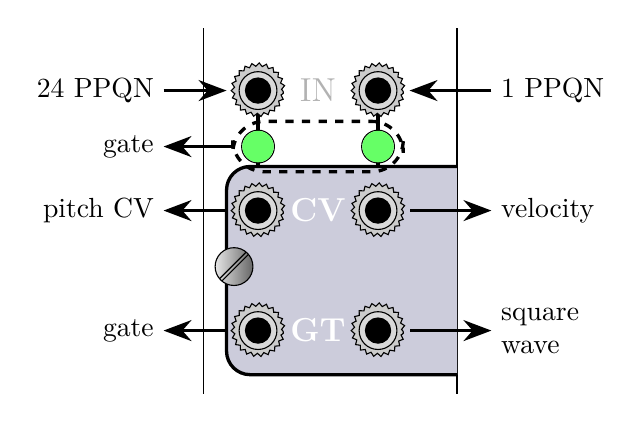
\begin{tikzpicture}[scale=0.8]
  {\setmainfont[Path={../../tsukurimashou/otf/},
BoldFont={TsukurimashouBokukkoExtraBoldPS}]{TsukurimashouBokukkoDemiboldPS}%
% start out defining coordinates
\coordinate (lbh) at (4.91mm,31.23mm) {};
\coordinate (j1) at (8.72mm,59.17mm) {};
\coordinate (j2) at (27.77mm,59.17mm) {};
\coordinate (j3) at (8.72mm,40.12mm) {};
\coordinate (j4) at (27.77mm,40.12mm) {};
\coordinate (j5) at (8.72mm,21.07mm) {};
\coordinate (j6) at (27.77mm,21.07mm) {};
\coordinate (d5) at (8.72mm,50.28mm) {};
\coordinate (d6) at (27.77mm,50.28mm) {};
%
\draw (0,11.07mm) -- (0,69.07mm);
\draw (40.30mm,11.07mm) -- (40.30mm,69.07mm);
%
\draw[very thick,black] (j1) -- (j3);
\draw[very thick,black] (j2) -- (j4);
\draw[very thick,black,fill=blue!30!black!20!white,rounded corners=3.0mm]
  (40.30mm,47.12mm) -- (3.72mm,47.12mm) --
  (3.72mm,14.07mm) -- (40.33mm,14.07mm);
\node[black!30!white] at ($(j1)!0.5!(j2)$) {\large IN};
\node[white] at ($(j3)!0.5!(j4)$) {\large\textbf{CV}};
\node[white] at ($(j5)!0.5!(j6)$) {\large\textbf{GT}};
%
% board-to-panel mounting holes, to clear M3 machine screw
\draw (lbh) circle[radius=1.60mm];
% six jacks with M6 threads, 6.3mm holes
\draw (j1) circle[radius=3.15mm];
\draw (j2) circle[radius=3.15mm];
\draw (j3) circle[radius=3.15mm];
\draw (j4) circle[radius=3.15mm];
\draw (j5) circle[radius=3.15mm];
\draw (j6) circle[radius=3.15mm];
% two LEDs, 5.20mm holes
\draw (d5) circle[radius=2.60mm];
\draw (d6) circle[radius=2.60mm];
%
% mock up screw heads, knobs
% machine screws with 6mm heads
\foreach \screwname in {lbh} {
  \path[draw=black,shading=ball,
    left color=black!10!white,right color=black!60!white]
    (\screwname) circle[radius=3mm];
  \draw ($(\screwname)+(50:3.0mm)$)--($(\screwname)+(220:3.0mm)$);
  \draw ($(\screwname)+(40:3.0mm)$)--($(\screwname)+(230:3.0mm)$);
}
% jacks with knurled nuts
\foreach \jackname in {j1,j2,j3,j4,j5,j6} {
  \path[draw=black,fill=black!20!white,
    decorate,decoration={snake,amplitude=0.6,segment length=2.5}]
    ($(\jackname)+(0,-0.15mm)$) circle[radius=4mm];
  \path[draw=black,fill=black!15!white] (\jackname) circle[radius=3mm];
  \path[draw=black,fill=black] (\jackname) circle[radius=2mm];
}
}

%
  \path[fill=green!60!white] (d5) circle[radius=2.50mm];
  \path[fill=green!60!white] (d6) circle[radius=2.50mm];
  \draw[very thick,-{Stealth[scale=1.2]}]
    ($(j1)+(-15mm,0)$) -- ($(j1)+(-5mm,0)$);
  \draw[very thick,-{Stealth[scale=1.2]}]
    ($(j2)+(18mm,0)$) -- ($(j2)+(5mm,0)$);
  \draw[very thick,{Stealth[scale=1.2]}-]
    ($(d5)+(-15mm,0)$) -- ($(d5)+(-4mm,0)$);
%  \draw[very thick,{Stealth[scale=1.2]}-]
%    ($(d6)+(18mm,0)$) -- ($(d6)+(4mm,0)$);
  \draw[rounded corners=4mm,very thick,dashed]
    ($(d5)+(-4mm,-4mm)$) rectangle ($(d6)+(4mm,4mm)$);
  \draw[very thick,{Stealth[scale=1.2]}-]
    ($(j3)+(-15mm,0)$) -- ($(j3)+(-5mm,0)$);
  \draw[very thick,{Stealth[scale=1.2]}-]
    ($(j4)+(18mm,0)$) -- ($(j4)+(5mm,0)$);
  \draw[very thick,{Stealth[scale=1.2]}-]
    ($(j5)+(-15mm,0)$) -- ($(j5)+(-5mm,0)$);
  \draw[very thick,{Stealth[scale=1.2]}-]
    ($(j6)+(18mm,0)$) -- ($(j6)+(5mm,0)$);
%
  \node[anchor=east] at ($(j1)+(-15mm,0)$) {24 PPQN};
  \node[anchor=west] at ($(j2)+(18mm,0)$) {1 PPQN};
  \node[anchor=east] at ($(d5)+(-15mm,0)$) {gate};
  \node[anchor=east] at ($(j3)+(-15mm,0)$) {pitch CV};
  \node[anchor=west] at ($(j4)+(18mm,0)$) {velocity};
  \node[anchor=east] at ($(j5)+(-15mm,0)$) {gate};
  \node[anchor=west] at ($(j6)+(18mm,0)$)
    {\parbox{12mm}{square wave}};
\end{tikzpicture}\par}

Channel 1 implements monophonic note stealing.  If a new note starts while
an old one is in progress, then the old note immediately ends and is
replaced by the new one.  In such a case the gate output goes low for
approximately 1ms to signal the start of the new note.

A stolen note ends when it is stolen.  For instance, if you play Note On C,
Note On G, Note Off G, then the gate goes low and the oscillator continues
playing G.  The C does not come back when the G ends, even if you still
have not yet played Note Off C.

Although in this mode the module does not \emph{use} its tempo clock, it can
\emph{accept} clock signals on the input jacks.  The left input jack accepts
a standard 24~PPQN MIDI clock.  The right input jack will function as a
1~PPQN or tap tempo input if there is nothing received on the left
input, or as a synchronization or reset input (marking the start of a
quarter note) when there is also a 24~PPQN clock being received on the left.

%%%%%%%%%%%%%%%%%%%%%%%%%%%%%%%%%%%%%%%%%%%%%%%%%%%%%%%%%%%%%%%%%%%%%%%%

\section{Channel 2:  duophonic CV/gate}

This mode is intended for controlling a synthesizer with two more or less
identical voices.  Each voice has a pitch CV and a gate CV, which respond to
Note On and Off messages for up to two simultaneous notes in the same MIDI
channel.

{\centering
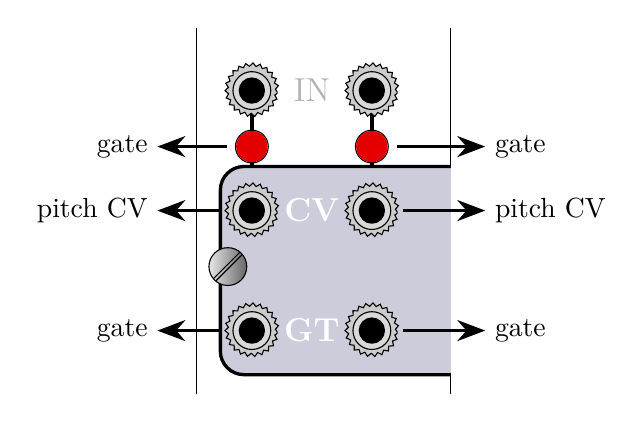
\begin{tikzpicture}[scale=0.8]
  {\setmainfont[Path={../../tsukurimashou/otf/},
BoldFont={TsukurimashouBokukkoExtraBoldPS}]{TsukurimashouBokukkoDemiboldPS}%
% start out defining coordinates
\coordinate (lbh) at (4.91mm,31.23mm) {};
\coordinate (j1) at (8.72mm,59.17mm) {};
\coordinate (j2) at (27.77mm,59.17mm) {};
\coordinate (j3) at (8.72mm,40.12mm) {};
\coordinate (j4) at (27.77mm,40.12mm) {};
\coordinate (j5) at (8.72mm,21.07mm) {};
\coordinate (j6) at (27.77mm,21.07mm) {};
\coordinate (d5) at (8.72mm,50.28mm) {};
\coordinate (d6) at (27.77mm,50.28mm) {};
%
\draw (0,11.07mm) -- (0,69.07mm);
\draw (40.30mm,11.07mm) -- (40.30mm,69.07mm);
%
\draw[very thick,black] (j1) -- (j3);
\draw[very thick,black] (j2) -- (j4);
\draw[very thick,black,fill=blue!30!black!20!white,rounded corners=3.0mm]
  (40.30mm,47.12mm) -- (3.72mm,47.12mm) --
  (3.72mm,14.07mm) -- (40.33mm,14.07mm);
\node[black!30!white] at ($(j1)!0.5!(j2)$) {\large IN};
\node[white] at ($(j3)!0.5!(j4)$) {\large\textbf{CV}};
\node[white] at ($(j5)!0.5!(j6)$) {\large\textbf{GT}};
%
% board-to-panel mounting holes, to clear M3 machine screw
\draw (lbh) circle[radius=1.60mm];
% six jacks with M6 threads, 6.3mm holes
\draw (j1) circle[radius=3.15mm];
\draw (j2) circle[radius=3.15mm];
\draw (j3) circle[radius=3.15mm];
\draw (j4) circle[radius=3.15mm];
\draw (j5) circle[radius=3.15mm];
\draw (j6) circle[radius=3.15mm];
% two LEDs, 5.20mm holes
\draw (d5) circle[radius=2.60mm];
\draw (d6) circle[radius=2.60mm];
%
% mock up screw heads, knobs
% machine screws with 6mm heads
\foreach \screwname in {lbh} {
  \path[draw=black,shading=ball,
    left color=black!10!white,right color=black!60!white]
    (\screwname) circle[radius=3mm];
  \draw ($(\screwname)+(50:3.0mm)$)--($(\screwname)+(220:3.0mm)$);
  \draw ($(\screwname)+(40:3.0mm)$)--($(\screwname)+(230:3.0mm)$);
}
% jacks with knurled nuts
\foreach \jackname in {j1,j2,j3,j4,j5,j6} {
  \path[draw=black,fill=black!20!white,
    decorate,decoration={snake,amplitude=0.6,segment length=2.5}]
    ($(\jackname)+(0,-0.15mm)$) circle[radius=4mm];
  \path[draw=black,fill=black!15!white] (\jackname) circle[radius=3mm];
  \path[draw=black,fill=black] (\jackname) circle[radius=2mm];
}
}

%
  \path[fill=red!90!black] (d5) circle[radius=2.50mm];
  \path[fill=red!90!black] (d6) circle[radius=2.50mm];
%  \draw[very thick,-{Stealth[scale=1.2]}]
%    ($(j1)+(-15mm,0)$) -- ($(j1)+(-5mm,0)$);
%  \draw[very thick,-{Stealth[scale=1.2]}]
%    ($(j2)+(18mm,0)$) -- ($(j2)+(5mm,0)$);
  \draw[very thick,{Stealth[scale=1.2]}-]
    ($(d5)+(-15mm,0)$) -- ($(d5)+(-4mm,0)$);
  \draw[very thick,{Stealth[scale=1.2]}-]
    ($(d6)+(18mm,0)$) -- ($(d6)+(4mm,0)$);
  \draw[very thick,{Stealth[scale=1.2]}-]
    ($(j3)+(-15mm,0)$) -- ($(j3)+(-5mm,0)$);
  \draw[very thick,{Stealth[scale=1.2]}-]
    ($(j4)+(18mm,0)$) -- ($(j4)+(5mm,0)$);
  \draw[very thick,{Stealth[scale=1.2]}-]
    ($(j5)+(-15mm,0)$) -- ($(j5)+(-5mm,0)$);
  \draw[very thick,{Stealth[scale=1.2]}-]
    ($(j6)+(18mm,0)$) -- ($(j6)+(5mm,0)$);
%
  \node[anchor=east] at ($(d5)+(-15mm,0)$) {gate};
  \node[anchor=west] at ($(d6)+(18mm,0)$) {gate};
  \node[anchor=east] at ($(j3)+(-15mm,0)$) {pitch CV};
  \node[anchor=west] at ($(j4)+(18mm,0)$) {pitch CV};
  \node[anchor=east] at ($(j5)+(-15mm,0)$) {gate};
  \node[anchor=west] at ($(j6)+(18mm,0)$) {gate};
\end{tikzpicture}\par}

Channel~2 implements note stealing according to these rules:
\begin{itemize}
\item The first note goes to the left.
\item If exactly one side is free, a new note goes there.
\item Otherwise (both sides free, or neither), a new note goes to the side
that least recently had a new note.
\end{itemize}

As with Channel~1, the gate CV drops for about 1ms when a new note replaces
an old one, so as to give some chance of retriggering whatever module is
using that gate signal.  Also as in Channel~1, stolen notes end when they
are stolen.

Signals on the input jacks are ignored in this mode, and the LED on each
side glows red when there is a note active on the side in question.  Pitch
bend in this channel affects both sides.

%%%%%%%%%%%%%%%%%%%%%%%%%%%%%%%%%%%%%%%%%%%%%%%%%%%%%%%%%%%%%%%%%%%%%%%%

\section{Channels 3 and 4:  quantize to MIDI}

When it receives MIDI notes in either of these two channels, the Gracious
Host acts as a dual quantizer.  The input voltage on each side is compared
to whichever MIDI notes are currently held, and the output pitch control
voltages are set to the voltages for the notes closest to the inputs.

{\centering
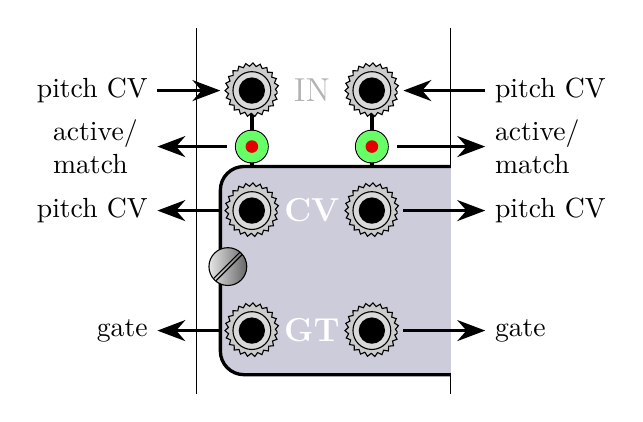
\begin{tikzpicture}[scale=0.8]
  {\setmainfont[Path={../../tsukurimashou/otf/},
BoldFont={TsukurimashouBokukkoExtraBoldPS}]{TsukurimashouBokukkoDemiboldPS}%
% start out defining coordinates
\coordinate (lbh) at (4.91mm,31.23mm) {};
\coordinate (j1) at (8.72mm,59.17mm) {};
\coordinate (j2) at (27.77mm,59.17mm) {};
\coordinate (j3) at (8.72mm,40.12mm) {};
\coordinate (j4) at (27.77mm,40.12mm) {};
\coordinate (j5) at (8.72mm,21.07mm) {};
\coordinate (j6) at (27.77mm,21.07mm) {};
\coordinate (d5) at (8.72mm,50.28mm) {};
\coordinate (d6) at (27.77mm,50.28mm) {};
%
\draw (0,11.07mm) -- (0,69.07mm);
\draw (40.30mm,11.07mm) -- (40.30mm,69.07mm);
%
\draw[very thick,black] (j1) -- (j3);
\draw[very thick,black] (j2) -- (j4);
\draw[very thick,black,fill=blue!30!black!20!white,rounded corners=3.0mm]
  (40.30mm,47.12mm) -- (3.72mm,47.12mm) --
  (3.72mm,14.07mm) -- (40.33mm,14.07mm);
\node[black!30!white] at ($(j1)!0.5!(j2)$) {\large IN};
\node[white] at ($(j3)!0.5!(j4)$) {\large\textbf{CV}};
\node[white] at ($(j5)!0.5!(j6)$) {\large\textbf{GT}};
%
% board-to-panel mounting holes, to clear M3 machine screw
\draw (lbh) circle[radius=1.60mm];
% six jacks with M6 threads, 6.3mm holes
\draw (j1) circle[radius=3.15mm];
\draw (j2) circle[radius=3.15mm];
\draw (j3) circle[radius=3.15mm];
\draw (j4) circle[radius=3.15mm];
\draw (j5) circle[radius=3.15mm];
\draw (j6) circle[radius=3.15mm];
% two LEDs, 5.20mm holes
\draw (d5) circle[radius=2.60mm];
\draw (d6) circle[radius=2.60mm];
%
% mock up screw heads, knobs
% machine screws with 6mm heads
\foreach \screwname in {lbh} {
  \path[draw=black,shading=ball,
    left color=black!10!white,right color=black!60!white]
    (\screwname) circle[radius=3mm];
  \draw ($(\screwname)+(50:3.0mm)$)--($(\screwname)+(220:3.0mm)$);
  \draw ($(\screwname)+(40:3.0mm)$)--($(\screwname)+(230:3.0mm)$);
}
% jacks with knurled nuts
\foreach \jackname in {j1,j2,j3,j4,j5,j6} {
  \path[draw=black,fill=black!20!white,
    decorate,decoration={snake,amplitude=0.6,segment length=2.5}]
    ($(\jackname)+(0,-0.15mm)$) circle[radius=4mm];
  \path[draw=black,fill=black!15!white] (\jackname) circle[radius=3mm];
  \path[draw=black,fill=black] (\jackname) circle[radius=2mm];
}
}

%
  \path[fill=green!60!white] (d5) circle[radius=2.50mm];
  \path[fill=green!60!white] (d6) circle[radius=2.50mm];
  \path[fill=red!90!black] (d5) circle[radius=1.0mm];
  \path[fill=red!90!black] (d6) circle[radius=1.0mm];
  \draw[very thick,-{Stealth[scale=1.2]}]
    ($(j1)+(-15mm,0)$) -- ($(j1)+(-5mm,0)$);
  \draw[very thick,-{Stealth[scale=1.2]}]
    ($(j2)+(18mm,0)$) -- ($(j2)+(5mm,0)$);
  \draw[very thick,{Stealth[scale=1.2]}-]
    ($(d5)+(-15mm,0)$) -- ($(d5)+(-4mm,0)$);
  \draw[very thick,{Stealth[scale=1.2]}-]
    ($(d6)+(18mm,0)$) -- ($(d6)+(4mm,0)$);
  \draw[very thick,{Stealth[scale=1.2]}-]
    ($(j3)+(-15mm,0)$) -- ($(j3)+(-5mm,0)$);
  \draw[very thick,{Stealth[scale=1.2]}-]
    ($(j4)+(18mm,0)$) -- ($(j4)+(5mm,0)$);
  \draw[very thick,{Stealth[scale=1.2]}-]
    ($(j5)+(-15mm,0)$) -- ($(j5)+(-5mm,0)$);
  \draw[very thick,{Stealth[scale=1.2]}-]
    ($(j6)+(18mm,0)$) -- ($(j6)+(5mm,0)$);
%
  \node[anchor=east] at ($(j1)+(-15mm,0)$) {pitch CV};
  \node[anchor=west] at ($(j2)+(18mm,0)$) {pitch CV};
  \node[anchor=east] at ($(d5)+(-15mm,0)$)
    {\parbox{12mm}{active/ match}};
  \node[anchor=west] at ($(d6)+(18mm,0)$)
    {\parbox{12mm}{active/ match}};
  \node[anchor=east] at ($(j3)+(-15mm,0)$) {pitch CV};
  \node[anchor=west] at ($(j4)+(18mm,0)$) {pitch CV};
  \node[anchor=east] at ($(j5)+(-15mm,0)$) {gate};
  \node[anchor=west] at ($(j6)+(18mm,0)$) {gate};
\end{tikzpicture}\par}

If, once in this mode, there happen to be no MIDI notes held, then all four
output voltages go to zero and the LEDs go dark.  Otherwise, the LED on each
side is red when the input happens to hit a quantized output value exactly
(that is, within the same semitone), and green otherwise.  Each gate output
is normally high when any notes are held, but it drops low for approximately
1ms when the associated pitch output goes to a new note, in order to allow
for retriggering of a synthesizer voice.

The difference between the two channels is that with Channel~3, quantization
is just to the received MIDI notes and no others.  With Channel~4, each
MIDI note counts as if you played it \emph{in every octave}.  So if you
play MIDI notes 60 and 69 (Middle C and the A above it, equivalent to output
voltages 2.00V and 2.75V) in Channel~3, then an input voltage of 0.50V
(equivalent to MIDI note 42) will quantize to 2.00V (MIDI note 60); but with
the same notes played in Channel~4, an input voltage of 0.50V will quantize
to 0.75V (MIDI note 45) because playing any C and A activates every C and A
as a possible quantization value.

Pitch bend, if nonzero, is applied to both outputs equally after
quantization; it does not affect the input quantization boundaries.  Some
future version of the firmware may attempt to do something more intelligent
with pitch bend, such as using it to support microtonal quantization.

%%%%%%%%%%%%%%%%%%%%%%%%%%%%%%%%%%%%%%%%%%%%%%%%%%%%%%%%%%%%%%%%%%%%%%%%

\section{Channels 5--7:  arpeggiator modes}

MIDI notes on these three channels will be arpeggiated to the CV and gate
outputs, in different styles depending on the channel.

{\centering
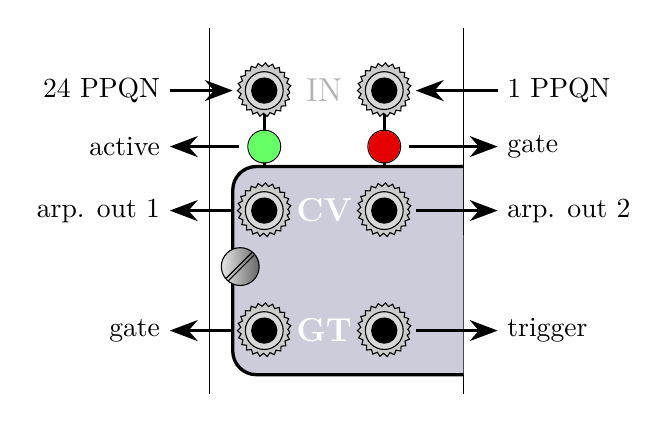
\begin{tikzpicture}[scale=0.8]
  {\setmainfont[Path={../../tsukurimashou/otf/},
BoldFont={TsukurimashouBokukkoExtraBoldPS}]{TsukurimashouBokukkoDemiboldPS}%
% start out defining coordinates
\coordinate (lbh) at (4.91mm,31.23mm) {};
\coordinate (j1) at (8.72mm,59.17mm) {};
\coordinate (j2) at (27.77mm,59.17mm) {};
\coordinate (j3) at (8.72mm,40.12mm) {};
\coordinate (j4) at (27.77mm,40.12mm) {};
\coordinate (j5) at (8.72mm,21.07mm) {};
\coordinate (j6) at (27.77mm,21.07mm) {};
\coordinate (d5) at (8.72mm,50.28mm) {};
\coordinate (d6) at (27.77mm,50.28mm) {};
%
\draw (0,11.07mm) -- (0,69.07mm);
\draw (40.30mm,11.07mm) -- (40.30mm,69.07mm);
%
\draw[very thick,black] (j1) -- (j3);
\draw[very thick,black] (j2) -- (j4);
\draw[very thick,black,fill=blue!30!black!20!white,rounded corners=3.0mm]
  (40.30mm,47.12mm) -- (3.72mm,47.12mm) --
  (3.72mm,14.07mm) -- (40.33mm,14.07mm);
\node[black!30!white] at ($(j1)!0.5!(j2)$) {\large IN};
\node[white] at ($(j3)!0.5!(j4)$) {\large\textbf{CV}};
\node[white] at ($(j5)!0.5!(j6)$) {\large\textbf{GT}};
%
% board-to-panel mounting holes, to clear M3 machine screw
\draw (lbh) circle[radius=1.60mm];
% six jacks with M6 threads, 6.3mm holes
\draw (j1) circle[radius=3.15mm];
\draw (j2) circle[radius=3.15mm];
\draw (j3) circle[radius=3.15mm];
\draw (j4) circle[radius=3.15mm];
\draw (j5) circle[radius=3.15mm];
\draw (j6) circle[radius=3.15mm];
% two LEDs, 5.20mm holes
\draw (d5) circle[radius=2.60mm];
\draw (d6) circle[radius=2.60mm];
%
% mock up screw heads, knobs
% machine screws with 6mm heads
\foreach \screwname in {lbh} {
  \path[draw=black,shading=ball,
    left color=black!10!white,right color=black!60!white]
    (\screwname) circle[radius=3mm];
  \draw ($(\screwname)+(50:3.0mm)$)--($(\screwname)+(220:3.0mm)$);
  \draw ($(\screwname)+(40:3.0mm)$)--($(\screwname)+(230:3.0mm)$);
}
% jacks with knurled nuts
\foreach \jackname in {j1,j2,j3,j4,j5,j6} {
  \path[draw=black,fill=black!20!white,
    decorate,decoration={snake,amplitude=0.6,segment length=2.5}]
    ($(\jackname)+(0,-0.15mm)$) circle[radius=4mm];
  \path[draw=black,fill=black!15!white] (\jackname) circle[radius=3mm];
  \path[draw=black,fill=black] (\jackname) circle[radius=2mm];
}
}

%
  \path[fill=green!60!white] (d5) circle[radius=2.50mm];
  \path[fill=red!90!black] (d6) circle[radius=2.50mm];
  \draw[very thick,-{Stealth[scale=1.2]}]
    ($(j1)+(-15mm,0)$) -- ($(j1)+(-5mm,0)$);
  \draw[very thick,-{Stealth[scale=1.2]}]
    ($(j2)+(18mm,0)$) -- ($(j2)+(5mm,0)$);
  \draw[very thick,{Stealth[scale=1.2]}-]
    ($(d5)+(-15mm,0)$) -- ($(d5)+(-4mm,0)$);
  \draw[very thick,{Stealth[scale=1.2]}-]
    ($(d6)+(18mm,0)$) -- ($(d6)+(4mm,0)$);
  \draw[very thick,{Stealth[scale=1.2]}-]
    ($(j3)+(-15mm,0)$) -- ($(j3)+(-5mm,0)$);
  \draw[very thick,{Stealth[scale=1.2]}-]
    ($(j4)+(18mm,0)$) -- ($(j4)+(5mm,0)$);
  \draw[very thick,{Stealth[scale=1.2]}-]
    ($(j5)+(-15mm,0)$) -- ($(j5)+(-5mm,0)$);
  \draw[very thick,{Stealth[scale=1.2]}-]
    ($(j6)+(18mm,0)$) -- ($(j6)+(5mm,0)$);
%
  \node[anchor=east] at ($(j1)+(-15mm,0)$) {24 PPQN};
  \node[anchor=west] at ($(j2)+(18mm,0)$) {1 PPQN};
  \node[anchor=east] at ($(d5)+(-15mm,0)$) {active};
  \node[anchor=west] at ($(d6)+(18mm,0)$) {gate};
  \node[anchor=east] at ($(j3)+(-15mm,0)$) {arp. out 1};
  \node[anchor=west] at ($(j4)+(18mm,0)$) {arp. out 2};
  \node[anchor=east] at ($(j5)+(-15mm,0)$) {gate};
  \node[anchor=west] at ($(j6)+(18mm,0)$) {trigger};
\end{tikzpicture}\par}

These channels use the global MIDI clock.  MIDI Timing Clock messages, or
pulses received on the left input jack, define the tempo at a rate of
24~PPQN.  MIDI Start messages reset to the start of the quarter note. 
Pulses received on the right input jack, and the tap tempo key on a typing
keyboard, reset to the start of the quarter note and also define the tempo
when there is no 24~PPQN clock.

The left digital output is the gate; it goes high (9V nominal) and the right
LED glows red, for the first 7/8 of each quarter note time.  The right
digital output produces a 960$\mu$s trigger at the start of each quarter
note time; this can also function as a 1~PPQN clock for other modules.  The
left LED glows green when there are any held notes, that is, when the
arpeggiator is active.  As for the CV outputs, they cycle through the held
MIDI notes in a way that depends on the channel.

Channel~5 arpeggiates up and down.  The left output cycles through the notes
upward (in order of increasing pitch) while the right output cycles
downward.

Channel~6 arpeggiates the held notes in the order they were entered, with
the right output one step ahead of the left.

Channel~7 arpeggiates in random order.  In more detail, the right output
selects one of the held notes uniformly at random on each beat.  That means
\emph{every} held note is available; the right output can repeat notes.  The
left output selects a note at random, but if there are at least two held
notes then it will avoid choosing the same note as the right output, and if
there are at least three held notes then it will also avoid its own previous
value; other than those exceptions, it selects uniformly.  So the left
output will not repeat notes, given sufficient held notes to choose from. 
The random numbers for Channel~7 come from a hashed entropy pool
continuously reseeded by I/O timings, and they should be random enough for
rock'n'roll even if not cryptographically certifiable.

All three arpeggiation modes start their new notes \emph{on the beat}.  If
you start playing notes into these channels when the tempo is slow, there
may be a noticeable delay before the output starts playing; but this design
feature is intended to allow playing more precisely \emph{with} the beat in
typical modular performance styles.  Note that the tempo clock needs to be
running in order for the arpeggiator to be useful.  To use these channels
you must provide the module with MIDI clock messages, a clock on the input
jacks, or tap tempo from a typing keyboard.

%%%%%%%%%%%%%%%%%%%%%%%%%%%%%%%%%%%%%%%%%%%%%%%%%%%%%%%%%%%%%%%%%%%%%%%%

\section{Channels 8 and 9:  dual mono}

These two channels work together to allow independent control of two GV/gate
synthesizer voices.  Unlike Channel~2, which automatically assigns incoming
notes to either channel, you can use this pair of channels to specify on
which side each note will play.  Channel~8 controls the left and Channel~9
the right.

{\centering
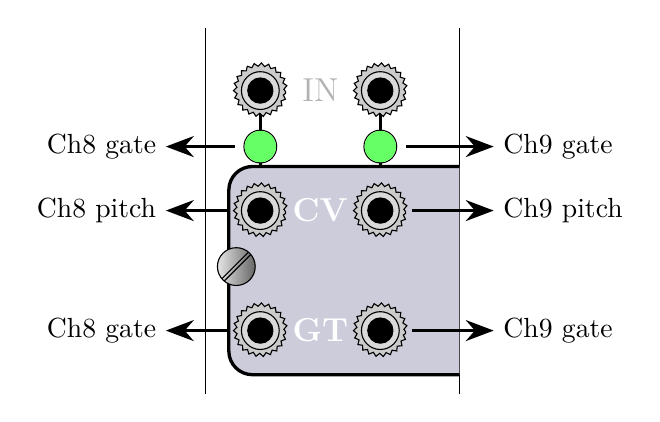
\begin{tikzpicture}[scale=0.8]
  {\setmainfont[Path={../../tsukurimashou/otf/},
BoldFont={TsukurimashouBokukkoExtraBoldPS}]{TsukurimashouBokukkoDemiboldPS}%
% start out defining coordinates
\coordinate (lbh) at (4.91mm,31.23mm) {};
\coordinate (j1) at (8.72mm,59.17mm) {};
\coordinate (j2) at (27.77mm,59.17mm) {};
\coordinate (j3) at (8.72mm,40.12mm) {};
\coordinate (j4) at (27.77mm,40.12mm) {};
\coordinate (j5) at (8.72mm,21.07mm) {};
\coordinate (j6) at (27.77mm,21.07mm) {};
\coordinate (d5) at (8.72mm,50.28mm) {};
\coordinate (d6) at (27.77mm,50.28mm) {};
%
\draw (0,11.07mm) -- (0,69.07mm);
\draw (40.30mm,11.07mm) -- (40.30mm,69.07mm);
%
\draw[very thick,black] (j1) -- (j3);
\draw[very thick,black] (j2) -- (j4);
\draw[very thick,black,fill=blue!30!black!20!white,rounded corners=3.0mm]
  (40.30mm,47.12mm) -- (3.72mm,47.12mm) --
  (3.72mm,14.07mm) -- (40.33mm,14.07mm);
\node[black!30!white] at ($(j1)!0.5!(j2)$) {\large IN};
\node[white] at ($(j3)!0.5!(j4)$) {\large\textbf{CV}};
\node[white] at ($(j5)!0.5!(j6)$) {\large\textbf{GT}};
%
% board-to-panel mounting holes, to clear M3 machine screw
\draw (lbh) circle[radius=1.60mm];
% six jacks with M6 threads, 6.3mm holes
\draw (j1) circle[radius=3.15mm];
\draw (j2) circle[radius=3.15mm];
\draw (j3) circle[radius=3.15mm];
\draw (j4) circle[radius=3.15mm];
\draw (j5) circle[radius=3.15mm];
\draw (j6) circle[radius=3.15mm];
% two LEDs, 5.20mm holes
\draw (d5) circle[radius=2.60mm];
\draw (d6) circle[radius=2.60mm];
%
% mock up screw heads, knobs
% machine screws with 6mm heads
\foreach \screwname in {lbh} {
  \path[draw=black,shading=ball,
    left color=black!10!white,right color=black!60!white]
    (\screwname) circle[radius=3mm];
  \draw ($(\screwname)+(50:3.0mm)$)--($(\screwname)+(220:3.0mm)$);
  \draw ($(\screwname)+(40:3.0mm)$)--($(\screwname)+(230:3.0mm)$);
}
% jacks with knurled nuts
\foreach \jackname in {j1,j2,j3,j4,j5,j6} {
  \path[draw=black,fill=black!20!white,
    decorate,decoration={snake,amplitude=0.6,segment length=2.5}]
    ($(\jackname)+(0,-0.15mm)$) circle[radius=4mm];
  \path[draw=black,fill=black!15!white] (\jackname) circle[radius=3mm];
  \path[draw=black,fill=black] (\jackname) circle[radius=2mm];
}
}

%
  \path[fill=green!60!white] (d5) circle[radius=2.50mm];
  \path[fill=green!60!white] (d6) circle[radius=2.50mm];
  \draw[very thick,{Stealth[scale=1.2]}-]
    ($(d5)+(-15mm,0)$) -- ($(d5)+(-4mm,0)$);
  \draw[very thick,{Stealth[scale=1.2]}-]
    ($(d6)+(18mm,0)$) -- ($(d6)+(4mm,0)$);
  \draw[very thick,{Stealth[scale=1.2]}-]
    ($(j3)+(-15mm,0)$) -- ($(j3)+(-5mm,0)$);
  \draw[very thick,{Stealth[scale=1.2]}-]
    ($(j4)+(18mm,0)$) -- ($(j4)+(5mm,0)$);
  \draw[very thick,{Stealth[scale=1.2]}-]
    ($(j5)+(-15mm,0)$) -- ($(j5)+(-5mm,0)$);
  \draw[very thick,{Stealth[scale=1.2]}-]
    ($(j6)+(18mm,0)$) -- ($(j6)+(5mm,0)$);
%
  \node[anchor=east] at ($(d5)+(-15mm,0)$) {Ch8 gate};
  \node[anchor=west] at ($(d6)+(18mm,0)$) {Ch9 gate};
  \node[anchor=east] at ($(j3)+(-15mm,0)$) {Ch8 pitch};
  \node[anchor=west] at ($(j4)+(18mm,0)$) {Ch9 pitch};
  \node[anchor=east] at ($(j5)+(-15mm,0)$) {Ch8 gate};
  \node[anchor=west] at ($(j6)+(18mm,0)$) {Ch9 gate};
\end{tikzpicture}\par}

Much like Channel~1, these channels do monophonic note stealing.  The
LED for each channel glows green when a note is playing.  The input jacks
are ignored.  Channels~8 and~9 have independent pitch bend.

%%%%%%%%%%%%%%%%%%%%%%%%%%%%%%%%%%%%%%%%%%%%%%%%%%%%%%%%%%%%%%%%%%%%%%%%

\section{Channels 10 and 11:  drum notes}

These channels map note numbers into pulses on the four output jacks. 
Channel~10 produces a trigger of approximately 1ms at the start of each
note, whereas Channel~11 produces a gate pulse, high as long as the note
lasts.

Note numbers translate to output jacks according to a somewhat complicated
mapping that is designed to work without needing special configuration on
many common MIDI controllers.  As a simple starting point, this
assignment of General MIDI drum notes to output jacks is one that works:
\begin{itemize}
\item MIDI note 36 (Bass Drum 1): lower right
\item MIDI note 38 (Acoustic Snare): upper left
\item MIDI note 40 (Electric Snare): upper right
\item MIDI note 42 (Closed Hi Hat): lower left
\end{itemize}

{\centering
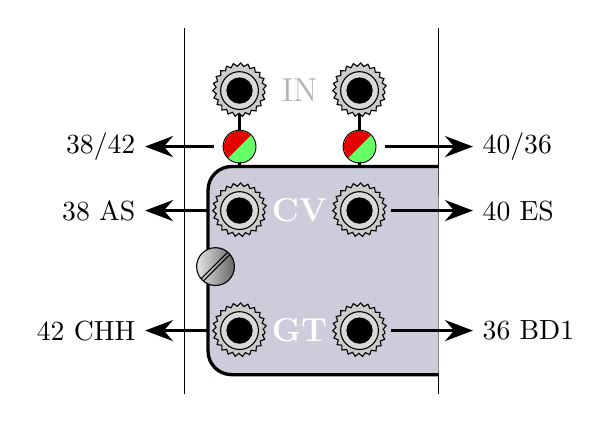
\begin{tikzpicture}[scale=0.8]
  {\setmainfont[Path={../../tsukurimashou/otf/},
BoldFont={TsukurimashouBokukkoExtraBoldPS}]{TsukurimashouBokukkoDemiboldPS}%
% start out defining coordinates
\coordinate (lbh) at (4.91mm,31.23mm) {};
\coordinate (j1) at (8.72mm,59.17mm) {};
\coordinate (j2) at (27.77mm,59.17mm) {};
\coordinate (j3) at (8.72mm,40.12mm) {};
\coordinate (j4) at (27.77mm,40.12mm) {};
\coordinate (j5) at (8.72mm,21.07mm) {};
\coordinate (j6) at (27.77mm,21.07mm) {};
\coordinate (d5) at (8.72mm,50.28mm) {};
\coordinate (d6) at (27.77mm,50.28mm) {};
%
\draw (0,11.07mm) -- (0,69.07mm);
\draw (40.30mm,11.07mm) -- (40.30mm,69.07mm);
%
\draw[very thick,black] (j1) -- (j3);
\draw[very thick,black] (j2) -- (j4);
\draw[very thick,black,fill=blue!30!black!20!white,rounded corners=3.0mm]
  (40.30mm,47.12mm) -- (3.72mm,47.12mm) --
  (3.72mm,14.07mm) -- (40.33mm,14.07mm);
\node[black!30!white] at ($(j1)!0.5!(j2)$) {\large IN};
\node[white] at ($(j3)!0.5!(j4)$) {\large\textbf{CV}};
\node[white] at ($(j5)!0.5!(j6)$) {\large\textbf{GT}};
%
% board-to-panel mounting holes, to clear M3 machine screw
\draw (lbh) circle[radius=1.60mm];
% six jacks with M6 threads, 6.3mm holes
\draw (j1) circle[radius=3.15mm];
\draw (j2) circle[radius=3.15mm];
\draw (j3) circle[radius=3.15mm];
\draw (j4) circle[radius=3.15mm];
\draw (j5) circle[radius=3.15mm];
\draw (j6) circle[radius=3.15mm];
% two LEDs, 5.20mm holes
\draw (d5) circle[radius=2.60mm];
\draw (d6) circle[radius=2.60mm];
%
% mock up screw heads, knobs
% machine screws with 6mm heads
\foreach \screwname in {lbh} {
  \path[draw=black,shading=ball,
    left color=black!10!white,right color=black!60!white]
    (\screwname) circle[radius=3mm];
  \draw ($(\screwname)+(50:3.0mm)$)--($(\screwname)+(220:3.0mm)$);
  \draw ($(\screwname)+(40:3.0mm)$)--($(\screwname)+(230:3.0mm)$);
}
% jacks with knurled nuts
\foreach \jackname in {j1,j2,j3,j4,j5,j6} {
  \path[draw=black,fill=black!20!white,
    decorate,decoration={snake,amplitude=0.6,segment length=2.5}]
    ($(\jackname)+(0,-0.15mm)$) circle[radius=4mm];
  \path[draw=black,fill=black!15!white] (\jackname) circle[radius=3mm];
  \path[draw=black,fill=black] (\jackname) circle[radius=2mm];
}
}

%
  \path[fill=green!60!white] (d5) circle[radius=2.50mm];
  \path[fill=red!90!black] ($(d5)+(225:2.5mm)$)
    arc[start angle=225,end angle=45,radius=2.50mm] --cycle;
  \path[fill=green!60!white] (d6) circle[radius=2.50mm];
  \path[fill=red!90!black] ($(d6)+(225:2.5mm)$)
    arc[start angle=225,end angle=45,radius=2.50mm] --cycle;
  \draw[very thick,{Stealth[scale=1.2]}-]
    ($(d5)+(-15mm,0)$) -- ($(d5)+(-4mm,0)$);
  \draw[very thick,{Stealth[scale=1.2]}-]
    ($(d6)+(18mm,0)$) -- ($(d6)+(4mm,0)$);
  \draw[very thick,{Stealth[scale=1.2]}-]
    ($(j3)+(-15mm,0)$) -- ($(j3)+(-5mm,0)$);
  \draw[very thick,{Stealth[scale=1.2]}-]
    ($(j4)+(18mm,0)$) -- ($(j4)+(5mm,0)$);
  \draw[very thick,{Stealth[scale=1.2]}-]
    ($(j5)+(-15mm,0)$) -- ($(j5)+(-5mm,0)$);
  \draw[very thick,{Stealth[scale=1.2]}-]
    ($(j6)+(18mm,0)$) -- ($(j6)+(5mm,0)$);
%
  \node[anchor=east] at ($(d5)+(-15mm,0)$) {38/42};
  \node[anchor=west] at ($(d6)+(18mm,0)$) {40/36};
  \node[anchor=east] at ($(j3)+(-15mm,0)$) {38 AS};
  \node[anchor=west] at ($(j4)+(18mm,0)$) {40 ES};
  \node[anchor=east] at ($(j5)+(-15mm,0)$) {42 CHH};
  \node[anchor=west] at ($(j6)+(18mm,0)$) {36 BD1};
\end{tikzpicture}\par}

Signals on the input jacks are ignored.  Each LED glows if any notes on
the corresponding side are active, red if the upper note (analog CV
output) is active and green if the lower but not the upper note is
active.

The upper analog outputs in drum mode go to their maximum voltage when high,
which is 5.5V nominal (uncalibrated).  The lower digital outputs, as usual,
go to about 9V.  The trigger pulse width is nominally 960$\mu$s.

Now, some more detail on how note mapping works.  Every MIDI note maps to one
of the four output jacks, so you can make up a mapping by choosing any four
notes that happen to map to different jacks.  If you have a controller like
a keyboard with many notes on it, you can probably find a usable mapping
quickly just through trial and error, but the scheme is designed to
guarantee that:
\begin{itemize}
\item any four consecutive MIDI notes starting with a multiple of four, such
as $\{0,1,2,3\}$ or $\{60,61,62,63\}$, will map to distinct jacks; and
\item any four MIDI notes spaced two apart, such as $\{0,2,4,6\}$ or
$\{65,67,69,71\}$, will map to distinct jacks.
\end{itemize}

That means pad controllers which typically assign the pads to consecutive
notes will often have four conveniently-arranged pads which control the four
output jacks.  It also means that the notes F, G, A, B (which are two
semitones apart) in any octave on a piano-style keyboard, or any four
horizontally adjacent keys on a Wicki-Hayden isomorphic keyboard (as
discussed in the typing-keyboard chapter of this manual), will work.

In even more detail:  each note number $N$ maps to a jack number $j=(\lfloor
N/4 \rfloor+N) \bmod 4$.  In words, that formula says to start with the note
number $N$, divide it by four and throw away the remainder, then add the
original $N$, divide the result by four again, and this time throw away the
quotient and look at only the remainder, which we'll call $j$.  Then:
\begin{itemize}
\item if $j=0$, the note activates the lower left jack;
\item if $j=1$, it activates the lower right jack;
\item if $j=2$, the upper left jack; and
\item if $j=3$, the upper right.
\end{itemize}

That splits the range of MIDI note numbers into four sets with the desired
properties of being hit by many convenient controller assignments.

{\centering
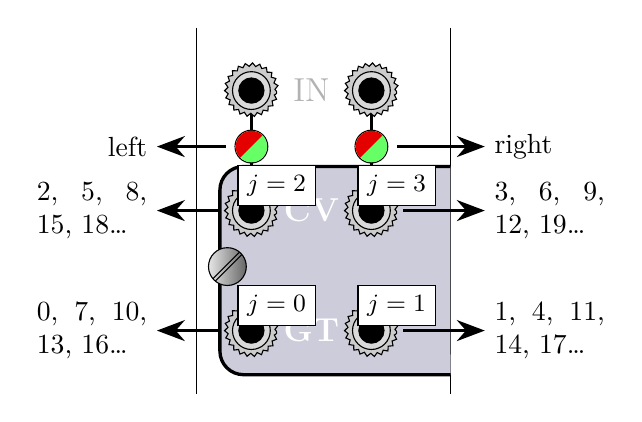
\begin{tikzpicture}[scale=0.8]
  {\setmainfont[Path={../../tsukurimashou/otf/},
BoldFont={TsukurimashouBokukkoExtraBoldPS}]{TsukurimashouBokukkoDemiboldPS}%
% start out defining coordinates
\coordinate (lbh) at (4.91mm,31.23mm) {};
\coordinate (j1) at (8.72mm,59.17mm) {};
\coordinate (j2) at (27.77mm,59.17mm) {};
\coordinate (j3) at (8.72mm,40.12mm) {};
\coordinate (j4) at (27.77mm,40.12mm) {};
\coordinate (j5) at (8.72mm,21.07mm) {};
\coordinate (j6) at (27.77mm,21.07mm) {};
\coordinate (d5) at (8.72mm,50.28mm) {};
\coordinate (d6) at (27.77mm,50.28mm) {};
%
\draw (0,11.07mm) -- (0,69.07mm);
\draw (40.30mm,11.07mm) -- (40.30mm,69.07mm);
%
\draw[very thick,black] (j1) -- (j3);
\draw[very thick,black] (j2) -- (j4);
\draw[very thick,black,fill=blue!30!black!20!white,rounded corners=3.0mm]
  (40.30mm,47.12mm) -- (3.72mm,47.12mm) --
  (3.72mm,14.07mm) -- (40.33mm,14.07mm);
\node[black!30!white] at ($(j1)!0.5!(j2)$) {\large IN};
\node[white] at ($(j3)!0.5!(j4)$) {\large\textbf{CV}};
\node[white] at ($(j5)!0.5!(j6)$) {\large\textbf{GT}};
%
% board-to-panel mounting holes, to clear M3 machine screw
\draw (lbh) circle[radius=1.60mm];
% six jacks with M6 threads, 6.3mm holes
\draw (j1) circle[radius=3.15mm];
\draw (j2) circle[radius=3.15mm];
\draw (j3) circle[radius=3.15mm];
\draw (j4) circle[radius=3.15mm];
\draw (j5) circle[radius=3.15mm];
\draw (j6) circle[radius=3.15mm];
% two LEDs, 5.20mm holes
\draw (d5) circle[radius=2.60mm];
\draw (d6) circle[radius=2.60mm];
%
% mock up screw heads, knobs
% machine screws with 6mm heads
\foreach \screwname in {lbh} {
  \path[draw=black,shading=ball,
    left color=black!10!white,right color=black!60!white]
    (\screwname) circle[radius=3mm];
  \draw ($(\screwname)+(50:3.0mm)$)--($(\screwname)+(220:3.0mm)$);
  \draw ($(\screwname)+(40:3.0mm)$)--($(\screwname)+(230:3.0mm)$);
}
% jacks with knurled nuts
\foreach \jackname in {j1,j2,j3,j4,j5,j6} {
  \path[draw=black,fill=black!20!white,
    decorate,decoration={snake,amplitude=0.6,segment length=2.5}]
    ($(\jackname)+(0,-0.15mm)$) circle[radius=4mm];
  \path[draw=black,fill=black!15!white] (\jackname) circle[radius=3mm];
  \path[draw=black,fill=black] (\jackname) circle[radius=2mm];
}
}

%
  \path[fill=green!60!white] (d5) circle[radius=2.50mm];
  \path[fill=red!90!black] ($(d5)+(225:2.5mm)$)
    arc[start angle=225,end angle=45,radius=2.50mm] --cycle;
  \path[fill=green!60!white] (d6) circle[radius=2.50mm];
  \path[fill=red!90!black] ($(d6)+(225:2.5mm)$)
    arc[start angle=225,end angle=45,radius=2.50mm] --cycle;
  \draw[very thick,{Stealth[scale=1.2]}-]
    ($(d5)+(-15mm,0)$) -- ($(d5)+(-4mm,0)$);
  \draw[very thick,{Stealth[scale=1.2]}-]
    ($(d6)+(18mm,0)$) -- ($(d6)+(4mm,0)$);
  \draw[very thick,{Stealth[scale=1.2]}-]
    ($(j3)+(-15mm,0)$) -- ($(j3)+(-5mm,0)$);
  \draw[very thick,{Stealth[scale=1.2]}-]
    ($(j4)+(18mm,0)$) -- ($(j4)+(5mm,0)$);
  \draw[very thick,{Stealth[scale=1.2]}-]
    ($(j5)+(-15mm,0)$) -- ($(j5)+(-5mm,0)$);
  \draw[very thick,{Stealth[scale=1.2]}-]
    ($(j6)+(18mm,0)$) -- ($(j6)+(5mm,0)$);
%
  \node[anchor=east] at ($(d5)+(-15mm,0)$) {left};
  \node[anchor=west] at ($(d6)+(18mm,0)$) {right};
  \node[anchor=east] at ($(j3)+(-15mm,0)$)
    {\parbox{14mm}{2, 5, 8, 15, 18\ldots}};
  \node[anchor=west] at ($(j4)+(18mm,0)$)
    {\parbox{14mm}{3, 6, 9, 12, 19\ldots}};
  \node[anchor=east] at ($(j5)+(-15mm,0)$)
    {\parbox{14mm}{0, 7, 10, 13, 16\ldots}};
  \node[anchor=west] at ($(j6)+(18mm,0)$)
    {\parbox{14mm}{1, 4, 11, 14, 17\ldots}};
  \node[draw,fill=white] at ($(j5)+(4mm,4mm)$) {\small $j=0$};
  \node[draw,fill=white] at ($(j6)+(4mm,4mm)$) {\small $j=1$};
  \node[draw,fill=white] at ($(j3)+(4mm,4mm)$) {\small $j=2$};
  \node[draw,fill=white] at ($(j4)+(4mm,4mm)$) {\small $j=3$};
\end{tikzpicture}\par}

%%%%%%%%%%%%%%%%%%%%%%%%%%%%%%%%%%%%%%%%%%%%%%%%%%%%%%%%%%%%%%%%%%%%%%%%

\section{Channel 12:  mono with clock out}

This monophonic mode provides CV/gate to control a synthesizer voice, with
output of the MIDI clock as Eurorack trigger signals.  The gate output is
sent through an analog output jack, meaning that its high level will be
approximately 5.5V.  The clock outputs are 960$\mu$s triggers with a high
level of approximately 9V, at 24~PPQN and 1~PPQN.  The 1~PPQN pulse is
scheduled about 1ms before the first 24~PPQN pulse of the quarter note, so
that it can be used as a ``reset''; these pulses are meant to express the
same semantics as the MIDI Timing Clock and MIDI Start messages.

The source for timing can be the input jacks, MIDI timing messages, or
the tap tempo feature of the typing keyboard driver.

{\centering
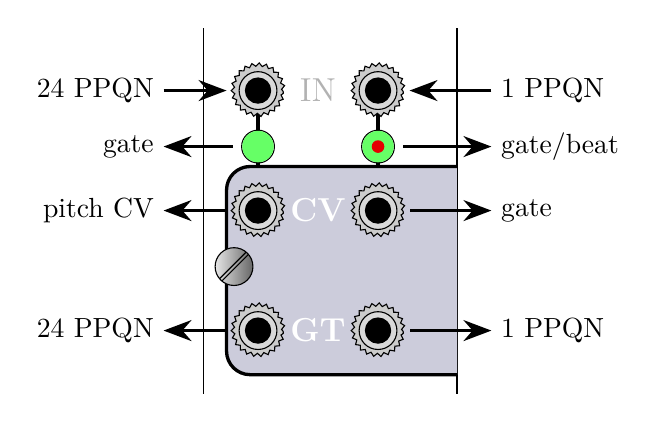
\begin{tikzpicture}[scale=0.8]
  {\setmainfont[Path={../../tsukurimashou/otf/},
BoldFont={TsukurimashouBokukkoExtraBoldPS}]{TsukurimashouBokukkoDemiboldPS}%
% start out defining coordinates
\coordinate (lbh) at (4.91mm,31.23mm) {};
\coordinate (j1) at (8.72mm,59.17mm) {};
\coordinate (j2) at (27.77mm,59.17mm) {};
\coordinate (j3) at (8.72mm,40.12mm) {};
\coordinate (j4) at (27.77mm,40.12mm) {};
\coordinate (j5) at (8.72mm,21.07mm) {};
\coordinate (j6) at (27.77mm,21.07mm) {};
\coordinate (d5) at (8.72mm,50.28mm) {};
\coordinate (d6) at (27.77mm,50.28mm) {};
%
\draw (0,11.07mm) -- (0,69.07mm);
\draw (40.30mm,11.07mm) -- (40.30mm,69.07mm);
%
\draw[very thick,black] (j1) -- (j3);
\draw[very thick,black] (j2) -- (j4);
\draw[very thick,black,fill=blue!30!black!20!white,rounded corners=3.0mm]
  (40.30mm,47.12mm) -- (3.72mm,47.12mm) --
  (3.72mm,14.07mm) -- (40.33mm,14.07mm);
\node[black!30!white] at ($(j1)!0.5!(j2)$) {\large IN};
\node[white] at ($(j3)!0.5!(j4)$) {\large\textbf{CV}};
\node[white] at ($(j5)!0.5!(j6)$) {\large\textbf{GT}};
%
% board-to-panel mounting holes, to clear M3 machine screw
\draw (lbh) circle[radius=1.60mm];
% six jacks with M6 threads, 6.3mm holes
\draw (j1) circle[radius=3.15mm];
\draw (j2) circle[radius=3.15mm];
\draw (j3) circle[radius=3.15mm];
\draw (j4) circle[radius=3.15mm];
\draw (j5) circle[radius=3.15mm];
\draw (j6) circle[radius=3.15mm];
% two LEDs, 5.20mm holes
\draw (d5) circle[radius=2.60mm];
\draw (d6) circle[radius=2.60mm];
%
% mock up screw heads, knobs
% machine screws with 6mm heads
\foreach \screwname in {lbh} {
  \path[draw=black,shading=ball,
    left color=black!10!white,right color=black!60!white]
    (\screwname) circle[radius=3mm];
  \draw ($(\screwname)+(50:3.0mm)$)--($(\screwname)+(220:3.0mm)$);
  \draw ($(\screwname)+(40:3.0mm)$)--($(\screwname)+(230:3.0mm)$);
}
% jacks with knurled nuts
\foreach \jackname in {j1,j2,j3,j4,j5,j6} {
  \path[draw=black,fill=black!20!white,
    decorate,decoration={snake,amplitude=0.6,segment length=2.5}]
    ($(\jackname)+(0,-0.15mm)$) circle[radius=4mm];
  \path[draw=black,fill=black!15!white] (\jackname) circle[radius=3mm];
  \path[draw=black,fill=black] (\jackname) circle[radius=2mm];
}
}

%
  \path[fill=green!60!white] (d5) circle[radius=2.50mm];
  \path[fill=green!60!white] (d6) circle[radius=2.50mm];
  \path[fill=red!90!black] (d6) circle[radius=1.0mm];
  \draw[very thick,-{Stealth[scale=1.2]}]
    ($(j1)+(-15mm,0)$) -- ($(j1)+(-5mm,0)$);
  \draw[very thick,-{Stealth[scale=1.2]}]
    ($(j2)+(18mm,0)$) -- ($(j2)+(5mm,0)$);
  \draw[very thick,{Stealth[scale=1.2]}-]
    ($(d5)+(-15mm,0)$) -- ($(d5)+(-4mm,0)$);
  \draw[very thick,{Stealth[scale=1.2]}-]
    ($(d6)+(18mm,0)$) -- ($(d6)+(4mm,0)$);
  \draw[very thick,{Stealth[scale=1.2]}-]
    ($(j3)+(-15mm,0)$) -- ($(j3)+(-5mm,0)$);
  \draw[very thick,{Stealth[scale=1.2]}-]
    ($(j4)+(18mm,0)$) -- ($(j4)+(5mm,0)$);
  \draw[very thick,{Stealth[scale=1.2]}-]
    ($(j5)+(-15mm,0)$) -- ($(j5)+(-5mm,0)$);
  \draw[very thick,{Stealth[scale=1.2]}-]
    ($(j6)+(18mm,0)$) -- ($(j6)+(5mm,0)$);
%
  \node[anchor=east] at ($(j1)+(-15mm,0)$) {24 PPQN};
  \node[anchor=west] at ($(j2)+(18mm,0)$) {1 PPQN};
  \node[anchor=east] at ($(d5)+(-15mm,0)$) {gate};
  \node[anchor=west] at ($(d6)+(18mm,0)$) {gate/beat};
  \node[anchor=east] at ($(j3)+(-15mm,0)$) {pitch CV};
  \node[anchor=west] at ($(j4)+(18mm,0)$) {gate};
  \node[anchor=east] at ($(j5)+(-15mm,0)$) {24 PPQN};
  \node[anchor=west] at ($(j6)+(18mm,0)$) {1 PPQN};
\end{tikzpicture}\par}

This channel implements monophonic note stealing, the same as Channel~1. 
Both LEDs glow green when a note is playing, but the right LED also flashes
red on the beat, overriding the green.

%%%%%%%%%%%%%%%%%%%%%%%%%%%%%%%%%%%%%%%%%%%%%%%%%%%%%%%%%%%%%%%%%%%%%%%%

\section{Channels 13--16:  reserved}

The last four channels are not currently implemented.  They are available
for use by future versions of the official firmware, or possibly by
user-defined firmware.

% $Id: qwerty.tex 9718 2021-12-19 19:26:46Z mskala $

%
% Typing (QWERTY) keyboard interface
% Copyright (C) 2022  Matthew Skala
%
% This program is free software: you can redistribute it and/or modify
% it under the terms of the GNU General Public License as published by
% the Free Software Foundation, version 3.
%
% This program is distributed in the hope that it will be useful,
% but WITHOUT ANY WARRANTY; without even the implied warranty of
% MERCHANTABILITY or FITNESS FOR A PARTICULAR PURPOSE.  See the
% GNU General Public License for more details.
%
% You should have received a copy of the GNU General Public License
% along with this program.  If not, see <http://www.gnu.org/licenses/>.
%
% Matthew Skala
% https://northcoastsynthesis.com/
% mskala@northcoastsynthesis.com
%

\newcommand{\myFlFl}{\raisebox{0.2ex}{\musDoubleFlat}}
\newcommand{\myFl}{\raisebox{0.2ex}{\musFlat}}
\newcommand{\mySh}{\raisebox{0.4ex}{\musSharp}}
\newcommand{\myShSh}{\raisebox{0.4ex}{\musDoubleSharp}}

\chapter{Typing keyboard interface}

The Gracious Host supports two kinds of USB keyboards:  musical keyboards
with a USB MIDI interface as described in the previous chapter, and the
other kind of keyboard that is commonly attached to a PC and used for
typing.  The driver for typing keyboards, described in this chapter, allows
them to be used for playing synthesizers -- with some limitations, but at a
much lower cost than most full-featured MIDI keyboards.

%%%%%%%%%%%%%%%%%%%%%%%%%%%%%%%%%%%%%%%%%%%%%%%%%%%%%%%%%%%%%%%%%%%%%%%%

\section{General comments on USB keyboards}

The typing keyboard driver supports what the USB standards call the ``boot
keyboard'' protocol.  In technical USB terms that means it will support a
USB device with an interface descriptor of class 3, subclass 1, protocol 1. 
This is the standard USB keyboard protocol used by the typing keyboards
people commonly plug into personal computers.  It is called ``boot
keyboard'' because the authors of the relevant standard apparently imagined
that the simple protocol would only be used by the BIOS configuration menus
of PCs, and most operating systems would instead use the ridiculously
complicated full-generality ``HID report protocol'' instead; but in fact,
most real-world implementations just use the boot keyboard protocol.

Wiring switches together to form a keyboard becomes more complicated if it
is desired to correctly detect when the user presses more than one key at
the same time.  In musical keyboards this issue is called ``polyphony'';
with typing keyboards, the same thing is called ``rollover.'' The USB boot
keyboard protocol is only capable of reporting to the host at most six
simultaneous keypresses (of regular typing keys; modifier keys like shift
are handled separately and do not count toward this limit) because it sends
six bytes of key information per report packet with each key consuming one
byte.  So a USB keyboard plugged into the Gracious Host can play \emph{at
most} six simultaneous MIDI notes in the ordinary way by pressing keys
at once.

However, reaching the limit requires keyboard hardware actually capable of
six-key rollover.  Some keyboards, especially fancier ones marketed as
``gaming'' keyboards, are able to do it; but cheaper generic USB keyboards
cannot really do full six-key rollover.  The average USB typing keyboard
that does not specifically advertise a rollover feature may give
incorrect results (not detecting some keys, or spuriously detecting
unpressed ``ghost'' keys) when multiple keys are pressed, usually depending
in a complicated way on the specific key combination involved.  The
Gracious Host only knows what the keyboard tells it, and cannot easily
compensate for such behaviour.

For the quantizer and arpeggiator features it's useful to play many notes at
once; so to get around both keyboard rollover limits and the user's limited
number of fingers, the Gracious Host typing-keyboard driver supports a
\emph{sustain} feature using the Caps Lock key to lock keys in a pressed
state without needing to hold them down.  See the section on that below.

USB typing keyboards have a limit on how fast they can be polled, and that
limits how responsive to keystrokes anything controlled by a USB typing
keyboard can be.  The limit depends on the specific keyboard model (the
keyboard decides how fast it will respond) but the default is usually
10ms intervals, for 100 polls per second.  There can also be a further delay
of a few milliseconds internal to the keyboard as the keyboard hardware
scans the array of switches.  Human beings are not capable of perceiving this
amount of so-called latency in keystroke response but many believe
they can, and users who hold that belief might prefer to use a USB MIDI
keyboard instead of a typing keyboard.  The USB MIDI protocol as implemented
by the Gracious Host allows for sub-millisecond polling.

The general layout of a USB typing keyboard is reasonably standardized, but
there are many small details that vary from one to another.  The biggest
distinction is between ``US-style'' keyboards, with a large L-shaped Enter
key, and ``ISO-style'' keyboards with a narrower vertical Enter key and a
few more small keys to accommodate the additional letters in non-English
languages.  The precise details of those keys, which letters are shown on
which keycaps, the locations of some punctuation marks like backslash, and
so on, vary a lot.  Keyboards do not report the details of their layout to a
USB host, so the host has to guess, maintain a database of specific keyboard
models, or be configured for it out-of-band.

The Gracious Host attempts to support all relevant keys that exist in most
popular keyboard layouts used around the world, with reasonable guesses as
to where they will be located; but be aware that it's possible your keyboard
will not actually have all the keys shown in the diagrams in this manual, or
that a few of them (especially around the edges of the main keyboard area)
will not be located exactly where they are shown.

The keys labelled ``GUI'' (and not implemented to do anything, in
the current firmware) are called that here because that's what they are
called in the relevant USB standard.  On most keyboards they are actually
labelled with the logo of an operating system vendor, like Microsoft or
Apple.

%%%%%%%%%%%%%%%%%%%%%%%%%%%%%%%%%%%%%%%%%%%%%%%%%%%%%%%%%%%%%%%%%%%%%%%%

\section{Piano-style keyboard layout}

Figure~\ref{fig:qwerty-layouts} shows two layouts.  The upper one is the
default layout active when a keyboard is first plugged into the Gracious
Host and the Num Lock LED is off.  Note names and MIDI note numbers
(assuming no octave shift) are as shown in the diagram.

\begin{sidewaysfigure*}
{\centering
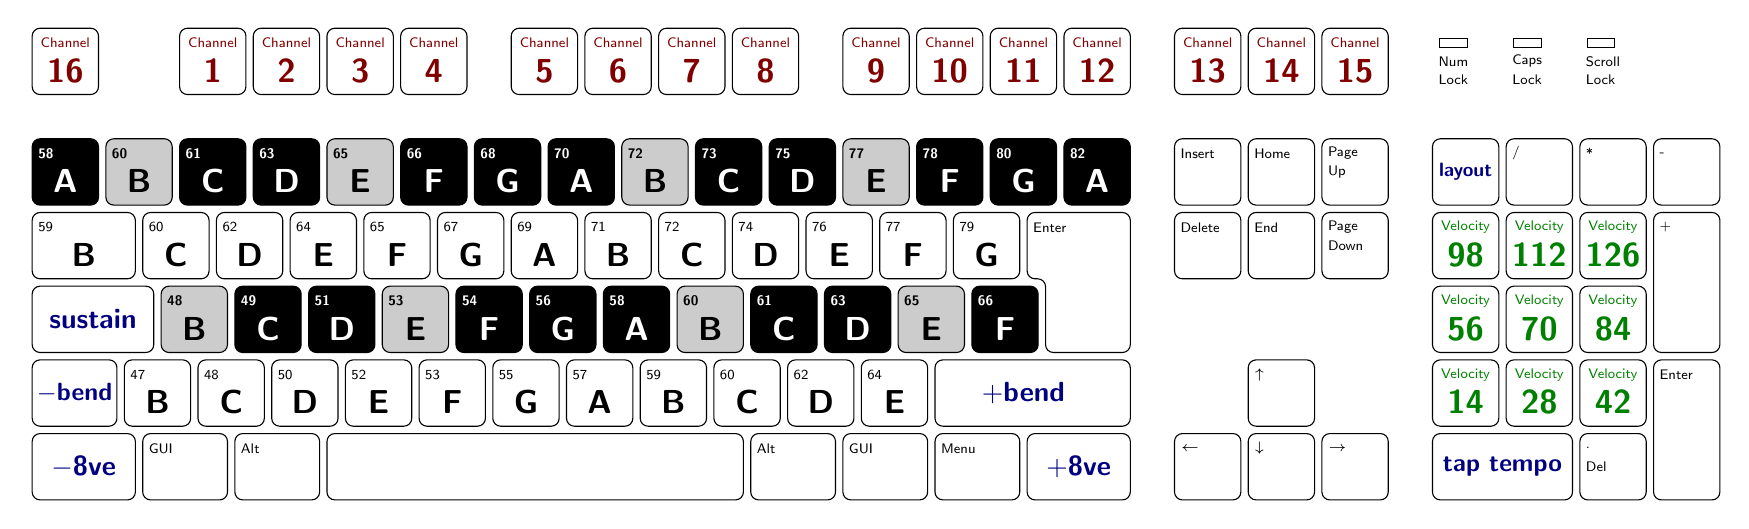
\begin{tikzpicture}[scale=0.234]
  % first row
  \foreach \xa/\xb/\tb in
    {0/4/16,
     8/12/1,12/16/2,16/20/3,20/24/4,
     26/30/5,30/34/6,34/38/7,38/42/8,
     44/48/9,48/52/10,52/56/11,56/60/12,
     62/66/13,66/70/14,70/74/15} {
    \draw[rounded corners={1mm}]
      ($(\xa,22)+(0.2,0.2)$) rectangle ($(\xb,26)+(-0.2,-0.2)$);
    \node[red!50!black] at ($(\xa,26)+(2,-1)$)
      {\tiny\textsf{Channel}};
    \node[red!50!black] at ($(\xa,22)+(2,1.5)$) {\large\bf\textsf{\tb}};
  }
  % LEDs
  \foreach \x/\t in {76/Num,80/Caps,84/Scroll} {
    \draw (\x+0.6,24.75) rectangle (\x+2.1,25.25);
    \node[anchor=west] at ($(\x,26)+(0,-2)$) {\tiny\textsf{\t}};
    \node[anchor=west] at ($(\x,26)+(0,-3)$) {\tiny\textsf{Lock}};
  }
  % second row, black note keys
  \foreach \xa/\xb/\ta/\tb in
    {0/4/58/{A\mySh},8/12/61/{C\mySh},12/16/63/{D\mySh},
     20/24/66/{F\mySh},24/28/68/{G\mySh},28/32/70/{A\mySh},
     36/40/73/{C\mySh},40/44/75/{D\mySh},48/52/78/{F\mySh},
     52/56/80/{G\mySh},56/60/82/{A\mySh}} {
    \draw[rounded corners={1mm},fill=black]
      ($(\xa,16)+(0.2,0.2)$) rectangle ($(\xb,20)+(-0.2,-0.2)$);
    \node[anchor=west,white] at ($(\xa,20)+(0,-1)$) {\tiny\bf\textsf{\ta}};
    \node[white] at ($(\xa,16)+(2,1.5)$) {\large\bf\textsf{\tb}};
  }
  % second row, skipped keys
  \foreach \xa/\xb/\ta/\tb in
    {4/8/60/{B\mySh},16/20/65/{E\mySh},32/36/72/{B\mySh},44/48/77/{E\mySh}} {
    \draw[rounded corners={1mm},fill=black!20!white]
      ($(\xa,16)+(0.2,0.2)$) rectangle ($(\xb,20)+(-0.2,-0.2)$);
    \node[anchor=west] at ($(\xa,20)+(0,-1)$) {\tiny\bf\textsf{\ta}};
    \node at ($(\xa,16)+(2,1.5)$) {\large\bf\textsf{\tb}};
  }
  % second row, non-note keys
  \foreach \xa/\xb/\ta/\tb in
    {62/66/Insert/{},66/70/Home/{},70/74/Page/Up,
     76/80/{}/{},80/84/{/}/{},84/88/*/{},88/92/-/{}} {
    \draw[rounded corners={1mm}]
      ($(\xa,16)+(0.2,0.2)$) rectangle ($(\xb,20)+(-0.2,-0.2)$);
    \node[anchor=west] at ($(\xa,20)+(0,-1)$) {\tiny\textsf{\ta}};
    \node[anchor=west] at ($(\xa,20)+(0,-2)$) {\tiny\textsf{\tb}};
  }
  % third row, white note keys
  \foreach \xa/\xb/\ta/\tb in
    {0/6/59/B,6/10/60/C,10/14/62/D,14/18/64/E,
     18/22/65/F,22/26/67/G,26/30/69/A,30/34/71/B,
     34/38/72/C,38/42/74/D,42/46/76/E,46/50/77/F,
     50/54/79/G} {
    \draw[rounded corners={1mm}]
      ($(\xa,12)+(0.2,0.2)$) rectangle ($(\xb,16)+(-0.2,-0.2)$);
    \node[anchor=west] at ($(\xa,16)+(0,-1)$) {\tiny\textsf{\ta}};
    \node at ($(\xa,12+1.5)!0.5!(\xb,12+1.5)$) {\large\bf\textsf{\tb}};
  }
  % third row, non-note keys
  \foreach \xa/\xb/\ta/\tb in
    {62/66/Delete/{},66/70/End/{},70/74/Page/Down} {
    \draw[rounded corners={1mm}]
      ($(\xa,12)+(0.2,0.2)$) rectangle ($(\xb,16)+(-0.2,-0.2)$);
    \node[anchor=west] at ($(\xa,16)+(0,-1)$) {\tiny\textsf{\ta}};
    \node[anchor=west] at ($(\xa,16)+(0,-2)$) {\tiny\textsf{\tb}};
  }
  % keys that span third and fourth rows
  \draw[rounded corners={1mm}]
    ($(55,8)+(0.2,0.2)$) -- ($(55,12)+(0.2,0.2)$) --
    ($(54,12)+(0.2,0.2)$) -- ($(54,16)+(0.2,-0.2)$) --
    ($(60,16)+(-0.2,-0.2)$) -- ($(60,8)+(-0.2,0.2)$) --cycle;
  \node[anchor=west] at ($(54,16)+(0,-1)$) {\tiny\textsf{Enter}};
  \draw[rounded corners={1mm}]
    ($(88,8)+(0.2,0.2)$) rectangle ($(92,16)+(-0.2,-0.2)$);
  \node[anchor=west] at ($(88,16)+(0,-1)$) {\tiny\textsf{+}};
  % fourth row, black note keys
  \foreach \xa/\xb/\ta/\tb in
    {11/15/49/{C\mySh},15/19/51/{D\mySh},
     23/27/54/{F\mySh},27/31/56/{G\mySh},31/35/58/{A\mySh},
     39/43/61/{C\mySh},43/47/63/{D\mySh},
     51/55/66/{F\mySh}} {
    \draw[rounded corners={1mm}, fill=black]
      ($(\xa,8)+(0.2,0.2)$) rectangle ($(\xb,12)+(-0.2,-0.2)$);
    \node[anchor=west,white] at ($(\xa,12)+(0,-1)$) {\tiny\bf\textsf{\ta}};
    \node[white] at ($(\xa,8)+(2,1.5)$) {\large\bf\textsf{\tb}};
  }
  % fourth row, skipped keys
  \foreach \xa/\xb/\ta/\tb in
    {7/11/48/{B\mySh},
     19/23/53/{E\mySh},
     35/39/60/{B\mySh},47/51/65/{E\mySh}} {
    \draw[rounded corners={1mm},fill=black!20!white]
      ($(\xa,8)+(0.2,0.2)$) rectangle ($(\xb,12)+(-0.2,-0.2)$);
    \node[anchor=west] at ($(\xa,12)+(0,-1)$) {\tiny\bf\textsf{\ta}};
    \node at ($(\xa,8)+(2,1.5)$) {\large\bf\textsf{\tb}};
  }
  % fourth row, non-note keys
  \foreach \xa/\xb/\ta/\tb in
    {0/7/{}/{}} {
    \draw[rounded corners={1mm}]
      ($(\xa,8)+(0.2,0.2)$) rectangle ($(\xb,12)+(-0.2,-0.2)$);
    \node[anchor=west] at ($(\xa,12)+(0,-1)$) {\tiny\textsf{\ta}};
    \node[anchor=west] at ($(\xa,12)+(0,-2)$) {\tiny\textsf{\tb}};
  }
  % fifth row, white note keys
  \foreach \xa/\xb/\ta/\tb in
    {5/9/47/B,9/13/48/C,13/17/50/D,17/21/52/E,
     21/25/53/F,25/29/55/G,29/33/57/A,33/37/59/B,
     37/41/60/C,41/45/62/D,45/49/64/E} {
    \draw[rounded corners={1mm}]
      ($(\xa,4)+(0.2,0.2)$) rectangle ($(\xb,8)+(-0.2,-0.2)$);
    \node[anchor=west] at ($(\xa,8)+(0,-1)$) {\tiny\textsf{\ta}};
    \node at ($(\xa,4+1.5)!0.5!(\xb,4+1.5)$) {\large\bf\textsf{\tb}};
  }
  % fifth row, non-note keys
  \foreach \xa/\xb/\ta/\tb in
    {0/5/{}/{},49/60/{}/{},
     66/70/{$\uparrow$}/{}} {
    \draw[rounded corners={1mm}]
      ($(\xa,4)+(0.2,0.2)$) rectangle ($(\xb,8)+(-0.2,-0.2)$);
    \node[anchor=west] at ($(\xa,8)+(0,-1)$) {\tiny\textsf{\ta}};
    \node[anchor=west] at ($(\xa,8)+(0,-2)$) {\tiny\textsf{\tb}};
  }
  % keys that span fifth and sixth rows
  \draw[rounded corners={1mm}]
    ($(88,0)+(0.2,0.2)$) rectangle ($(92,8)+(-0.2,-0.2)$);
  \node[anchor=west] at ($(88,8)+(0,-1)$) {\tiny\textsf{Enter}};
  % sixth row
  \foreach \xa/\xb/\ta/\tb in
    {0/6/{}/{},6/11/GUI/{},11/16/Alt/{},16/39/{}/{},
     39/44/Alt/{},44/49/GUI/{},49/54/Menu/{},54/60/{}/{},
     62/66/{$\leftarrow$}/{},66/70/{$\downarrow$}/{},70/74/{$\rightarrow$}/{},
     76/84/{}/{},84/88/./Del} {
    \draw[rounded corners={1mm}]
      ($(\xa,0)+(0.2,0.2)$) rectangle ($(\xb,4)+(-0.2,-0.2)$);
    \node[anchor=west] at ($(\xa,4)+(0,-1)$) {\tiny\textsf{\ta}};
    \node[anchor=west] at ($(\xa,4)+(0,-2)$) {\tiny\textsf{\tb}};
  }
  % keypad numerals
  \foreach \x/\y/\t in {76/4/14,80/4/28,84/4/42,76/8/56,80/8/70,
    84/8/84,76/12/98,80/12/112,84/12/126} {
    \draw[rounded corners={1mm}]
      ($(\x,\y)+(0.2,0.2)$) rectangle ($(\x+4,\y+4)+(-0.2,-0.2)$);
    \node[green!50!black] at ($(\x,\y)+(2,3)$)
      {\tiny\textsf{Velocity}};
    \node[green!50!black] at ($(\x,\y)+(2,1.5)$) {\large\bf\textsf{\t}};
  }
  % additional key labels
  \node[blue!50!black] at (3.5,10) {\bf\textsf{sustain}};
  \node[blue!50!black] at (2.5,6) {\small\bf\textsf{$-$bend}};
  \node[blue!50!black] at (3,2) {\bf\textsf{$-$8ve}};
  \node[blue!50!black] at (54,6) {\bf\textsf{$+$bend}};
  \node[blue!50!black] at (57,2) {\bf\textsf{$+$8ve}};
  \node[blue!50!black] at (78,18) {\scriptsize\bf\textsf{layout}};
  \node[blue!50!black] at (80,2) {\small\bf\textsf{tap tempo}};
\end{tikzpicture}\par
\vspace*{60pt}
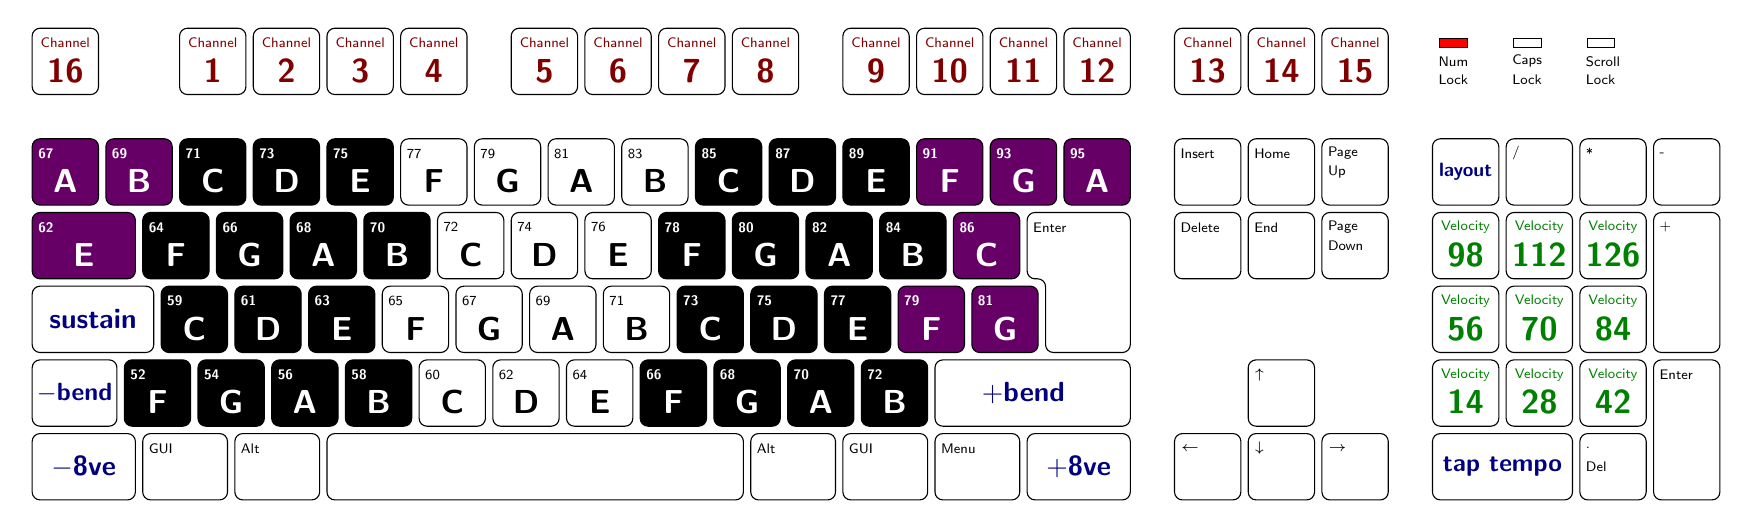
\begin{tikzpicture}[scale=0.234]
  % first row
  \foreach \xa/\xb/\tb in
    {0/4/16,
     8/12/1,12/16/2,16/20/3,20/24/4,
     26/30/5,30/34/6,34/38/7,38/42/8,
     44/48/9,48/52/10,52/56/11,56/60/12,
     62/66/13,66/70/14,70/74/15} {
    \draw[rounded corners={1mm}]
      ($(\xa,22)+(0.2,0.2)$) rectangle ($(\xb,26)+(-0.2,-0.2)$);
    \node[red!50!black] at ($(\xa,26)+(2,-1)$)
      {\tiny\textsf{Channel}};
    \node[red!50!black] at ($(\xa,22)+(2,1.5)$) {\large\bf\textsf{\tb}};
  }
  % LEDs
  \foreach \x/\t in {80/Caps,84/Scroll} {
    \draw (\x+0.6,24.75) rectangle (\x+2.1,25.25);
    \node[anchor=west] at ($(\x,26)+(0,-2)$) {\tiny\textsf{\t}};
    \node[anchor=west] at ($(\x,26)+(0,-3)$) {\tiny\textsf{Lock}};
  }
  \draw[fill=red] (76+0.6,24.75) rectangle (76+2.1,25.25);
  \node[anchor=west] at ($(76,26)+(0,-2)$) {\tiny\textsf{Num}};
  \node[anchor=west] at ($(76,26)+(0,-3)$) {\tiny\textsf{Lock}};
  % second row, purple note keys
  \foreach \xa/\xb/\ta/\tb in
    {0/4/67/{A\myFlFl},4/8/69/{B\myFlFl},48/52/91/{F\myShSh},
     52/56/93/{G\myShSh},56/60/95/{A\myShSh}} {
    \draw[rounded corners={1mm},fill=red!50!blue!80!black]
      ($(\xa,16)+(0.2,0.2)$) rectangle ($(\xb,20)+(-0.2,-0.2)$);
    \node[anchor=west,white] at ($(\xa,20)+(0,-1)$) {\tiny\bf\textsf{\ta}};
    \node[white] at ($(\xa,16)+(2,1.5)$) {\large\bf\textsf{\tb}};
  }
  % second row, black note keys
  \foreach \xa/\xb/\ta/\tb in
    {8/12/71/{C\myFl},12/16/73/{D\myFl},16/20/75/{E\myFl},
     36/40/85/{C\mySh},40/44/87/{D\mySh},44/48/89/{E\mySh}} {
    \draw[rounded corners={1mm},fill=black]
      ($(\xa,16)+(0.2,0.2)$) rectangle ($(\xb,20)+(-0.2,-0.2)$);
    \node[anchor=west,white] at ($(\xa,20)+(0,-1)$) {\tiny\bf\textsf{\ta}};
    \node[white] at ($(\xa,16)+(2,1.5)$) {\large\bf\textsf{\tb}};
  }
  % second row, white note keys
  \foreach \xa/\xb/\ta/\tb in
    {20/24/77/F,24/28/79/G,28/32/81/A,32/36/83/B} {
    \draw[rounded corners={1mm}]
      ($(\xa,16)+(0.2,0.2)$) rectangle ($(\xb,20)+(-0.2,-0.2)$);
    \node[anchor=west] at ($(\xa,20)+(0,-1)$) {\tiny\textsf{\ta}};
    \node at ($(\xa,16)+(2,1.5)$) {\large\bf\textsf{\tb}};
  }
  % second row, non-note keys
  \foreach \xa/\xb/\ta/\tb in
    {62/66/Insert/{},66/70/Home/{},70/74/Page/Up,
     76/80/{}/{},80/84/{/}/{},84/88/*/{},88/92/-/{}} {
    \draw[rounded corners={1mm}]
      ($(\xa,16)+(0.2,0.2)$) rectangle ($(\xb,20)+(-0.2,-0.2)$);
    \node[anchor=west] at ($(\xa,20)+(0,-1)$) {\tiny\textsf{\ta}};
    \node[anchor=west] at ($(\xa,20)+(0,-2)$) {\tiny\textsf{\tb}};
  }
  % third row, purple note keys
  \foreach \xa/\xb/\ta/\tb in
    {0/6/62/{E\myFlFl},50/54/86/{C\myShSh}} {
    \draw[rounded corners={1mm},fill=red!50!blue!80!black]
      ($(\xa,12)+(0.2,0.2)$) rectangle ($(\xb,16)+(-0.2,-0.2)$);
    \node[anchor=west,white] at ($(\xa,16)+(0,-1)$) {\tiny\bf\textsf{\ta}};
    \node[white] at ($(\xa,12+1.5)!0.5!(\xb,12+1.5)$) {\large\bf\textsf{\tb}};
  }
  % third row, black note keys
  \foreach \xa/\xb/\ta/\tb in
    {6/10/64/{F\myFl},10/14/66/{G\myFl},14/18/68/{A\myFl},18/22/70/{B\myFl},
     34/38/78/{F\mySh},38/42/80/{G\mySh},42/46/82/{A\mySh},46/50/84/{B\mySh}} {
    \draw[rounded corners={1mm},fill=black]
      ($(\xa,12)+(0.2,0.2)$) rectangle ($(\xb,16)+(-0.2,-0.2)$);
    \node[anchor=west,white] at ($(\xa,16)+(0,-1)$) {\tiny\bf\textsf{\ta}};
    \node[white] at ($(\xa,12+1.5)!0.5!(\xb,12+1.5)$) {\large\bf\textsf{\tb}};
  }
  % third row, white note keys
  \foreach \xa/\xb/\ta/\tb in
    {22/26/72/C,26/30/74/D,30/34/76/E} {
    \draw[rounded corners={1mm}]
      ($(\xa,12)+(0.2,0.2)$) rectangle ($(\xb,16)+(-0.2,-0.2)$);
    \node[anchor=west] at ($(\xa,16)+(0,-1)$) {\tiny\textsf{\ta}};
    \node at ($(\xa,12+1.5)!0.5!(\xb,12+1.5)$) {\large\bf\textsf{\tb}};
  }
  % third row, non-note keys
  \foreach \xa/\xb/\ta/\tb in
    {62/66/Delete/{},66/70/End/{},70/74/Page/Down} {
    \draw[rounded corners={1mm}]
      ($(\xa,12)+(0.2,0.2)$) rectangle ($(\xb,16)+(-0.2,-0.2)$);
    \node[anchor=west] at ($(\xa,16)+(0,-1)$) {\tiny\textsf{\ta}};
    \node[anchor=west] at ($(\xa,16)+(0,-2)$) {\tiny\textsf{\tb}};
  }
  % keys that span third and fourth rows
  \draw[rounded corners={1mm}]
    ($(55,8)+(0.2,0.2)$) -- ($(55,12)+(0.2,0.2)$) --
    ($(54,12)+(0.2,0.2)$) -- ($(54,16)+(0.2,-0.2)$) --
    ($(60,16)+(-0.2,-0.2)$) -- ($(60,8)+(-0.2,0.2)$) --cycle;
  \node[anchor=west] at ($(54,16)+(0,-1)$) {\tiny\textsf{Enter}};
  \draw[rounded corners={1mm}]
    ($(88,8)+(0.2,0.2)$) rectangle ($(92,16)+(-0.2,-0.2)$);
  \node[anchor=west] at ($(88,16)+(0,-1)$) {\tiny\textsf{+}};
  % fourth row, purple note keys
  \foreach \xa/\xb/\ta/\tb in
    {47/51/79/{F\myShSh},51/55/81/{G\myShSh}} {
    \draw[rounded corners={1mm},fill=red!50!blue!80!black]
      ($(\xa,8)+(0.2,0.2)$) rectangle ($(\xb,12)+(-0.2,-0.2)$);
    \node[anchor=west,white] at ($(\xa,12)+(0,-1)$) {\tiny\bf\textsf{\ta}};
    \node[white] at ($(\xa,8+1.5)!0.5!(\xb,8+1.5)$) {\large\bf\textsf{\tb}};
  }
  % fourth row, black note keys
  \foreach \xa/\xb/\ta/\tb in
    {7/11/59/{C\myFl},11/15/61/{D\myFl},15/19/63/{E\myFl},
     35/39/73/{C\mySh},39/43/75/{D\mySh},43/47/77/{E\mySh}} {
    \draw[rounded corners={1mm},fill=black]
      ($(\xa,8)+(0.2,0.2)$) rectangle ($(\xb,12)+(-0.2,-0.2)$);
    \node[anchor=west,white] at ($(\xa,12)+(0,-1)$) {\tiny\bf\textsf{\ta}};
    \node[white] at ($(\xa,8+1.5)!0.5!(\xb,8+1.5)$) {\large\bf\textsf{\tb}};
  }
  % fourth row, white note keys
  \foreach \xa/\xb/\ta/\tb in
    {0/7/{}/{},19/23/65/F,23/27/67/G,27/31/69/A,31/35/71/B} {
    \draw[rounded corners={1mm}]
      ($(\xa,8)+(0.2,0.2)$) rectangle ($(\xb,12)+(-0.2,-0.2)$);
    \node[anchor=west] at ($(\xa,12)+(0,-1)$) {\tiny\textsf{\ta}};
    \node at ($(\xa,8+1.5)!0.5!(\xb,8+1.5)$) {\large\bf\textsf{\tb}};
  }
  % fifth row, black note keys
  \foreach \xa/\xb/\ta/\tb in
    {5/9/52/{F\myFl},9/13/54/{G\myFl},13/17/56/{A\myFl},17/21/58/{B\myFl},
     33/37/66/{F\mySh},37/41/68/{G\mySh},41/45/70/{A\mySh},45/49/72/{B\mySh}} {
    \draw[rounded corners={1mm},fill=black]
      ($(\xa,4)+(0.2,0.2)$) rectangle ($(\xb,8)+(-0.2,-0.2)$);
    \node[anchor=west,white] at ($(\xa,8)+(0,-1)$) {\tiny\bf\textsf{\ta}};
    \node[white] at ($(\xa,4+1.5)!0.5!(\xb,4+1.5)$) {\large\bf\textsf{\tb}};
  }
  % fifth row, white note keys
  \foreach \xa/\xb/\ta/\tb in
    {21/25/60/C,25/29/62/D,29/33/64/E} {
    \draw[rounded corners={1mm}]
      ($(\xa,4)+(0.2,0.2)$) rectangle ($(\xb,8)+(-0.2,-0.2)$);
    \node[anchor=west] at ($(\xa,8)+(0,-1)$) {\tiny\textsf{\ta}};
    \node at ($(\xa,4+1.5)!0.5!(\xb,4+1.5)$) {\large\bf\textsf{\tb}};
  }
  % fifth row, non-note keys
  \foreach \xa/\xb/\ta/\tb in
    {0/5/{}/{},49/60/{}/{},
     66/70/{$\uparrow$}/{}} {
    \draw[rounded corners={1mm}]
      ($(\xa,4)+(0.2,0.2)$) rectangle ($(\xb,8)+(-0.2,-0.2)$);
    \node[anchor=west] at ($(\xa,8)+(0,-1)$) {\tiny\textsf{\ta}};
    \node[anchor=west] at ($(\xa,8)+(0,-2)$) {\tiny\textsf{\tb}};
  }
  % keys that span fifth and sixth rows
  \draw[rounded corners={1mm}]
    ($(88,0)+(0.2,0.2)$) rectangle ($(92,8)+(-0.2,-0.2)$);
  \node[anchor=west] at ($(88,8)+(0,-1)$) {\tiny\textsf{Enter}};
  % sixth row
  \foreach \xa/\xb/\ta/\tb in
    {0/6/{}/{},6/11/GUI/{},11/16/Alt/{},16/39/{}/{},
     39/44/Alt/{},44/49/GUI/{},49/54/Menu/{},54/60/{}/{},
     62/66/{$\leftarrow$}/{},66/70/{$\downarrow$}/{},70/74/{$\rightarrow$}/{},
     76/84/{}/{},84/88/./Del} {
    \draw[rounded corners={1mm}]
      ($(\xa,0)+(0.2,0.2)$) rectangle ($(\xb,4)+(-0.2,-0.2)$);
    \node[anchor=west] at ($(\xa,4)+(0,-1)$) {\tiny\textsf{\ta}};
    \node[anchor=west] at ($(\xa,4)+(0,-2)$) {\tiny\textsf{\tb}};
  }
  % keypad numerals
  \foreach \x/\y/\t in {76/4/14,80/4/28,84/4/42,76/8/56,80/8/70,
    84/8/84,76/12/98,80/12/112,84/12/126} {
    \draw[rounded corners={1mm}]
      ($(\x,\y)+(0.2,0.2)$) rectangle ($(\x+4,\y+4)+(-0.2,-0.2)$);
    \node[green!50!black] at ($(\x,\y)+(2,3)$)
      {\tiny\textsf{Velocity}};
    \node[green!50!black] at ($(\x,\y)+(2,1.5)$) {\large\bf\textsf{\t}};
  }
  % additional key labels
  \node[blue!50!black] at (3.5,10) {\bf\textsf{sustain}};
  \node[blue!50!black] at (2.5,6) {\small\bf\textsf{$-$bend}};
  \node[blue!50!black] at (3,2) {\bf\textsf{$-$8ve}};
  \node[blue!50!black] at (54,6) {\bf\textsf{$+$bend}};
  \node[blue!50!black] at (57,2) {\bf\textsf{$+$8ve}};
  \node[blue!50!black] at (78,18) {\scriptsize\bf\textsf{layout}};
  \node[blue!50!black] at (80,2) {\small\bf\textsf{tap tempo}};
\end{tikzpicture}\par
\vspace*{24pt}}
\caption{Keyboard layouts.}\label{fig:qwerty-layouts}
\end{sidewaysfigure*}

This layout is meant to imitate a piano's keyboard layout, with a little
over 2$\tfrac{1}{2}$ octaves of coverage.  Keys that fall into gaps of the
piano layout (shown in grey) are assigned to B$\musSharp$ and E$\musSharp$
(enharmonic to C and F) to make a consistent pattern.  The upper left of the
main letter area (Q on a QWERTY layout) is Middle~C, and the F key in a
QWERTY layout, which often has a tactile guide bump on it, is effectively an
F (shown as E$\musSharp$, but the same MIDI number).

%%%%%%%%%%%%%%%%%%%%%%%%%%%%%%%%%%%%%%%%%%%%%%%%%%%%%%%%%%%%%%%%%%%%%%%%

\section{Wicki-Hayden isomorphic layout}

Press Num Lock to switch layouts.  With the Num Lock LED glowing, the
Gracious Host implements a Wicki-Hayden isomorphic keyboard layout, as shown
in the lower half of Figure~\ref{fig:qwerty-layouts}.  This layout is named
after Kaspar Wicki and Brian Hayden, who independently invented and patented
it in 1896 and 1986 respectively.  It is similar to the layout commonly used
for concertina keyboards.

The Wicki-Hayden layout treats the keys as an hexagonal grid. 
Horizontally adjacent keys are a major second (two semitones) apart, pitch
going up from left to right across the keyboard.  From any note the
diagonally adjacent notes to the right represent the fifth of the note, in
the higher or lower octave according to whether they are diagonally up
and right or down and right.  Similarly, the diagonal notes to the left are
the fourth of the current note.  And going directly up or down two rows
corresponds to going up or down by a whole octave.

{\center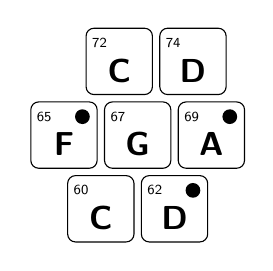
\begin{tikzpicture}[scale=0.234]
  \foreach \xa/\xb/\ta/\tb in
    {22/26/72/C,26/30/74/D} {
    \draw[rounded corners={1mm}]
      ($(\xa,12)+(0.2,0.2)$) rectangle ($(\xb,16)+(-0.2,-0.2)$);
    \node[anchor=west] at ($(\xa,16)+(0,-1)$) {\tiny\textsf{\ta}};
    \node at ($(\xa,12+1.5)!0.5!(\xb,12+1.5)$) {\large\bf\textsf{\tb}};
  }
  \foreach \xa/\xb/\ta/\tb in
    {19/23/65/F,23/27/67/G,27/31/69/A} {
    \draw[rounded corners={1mm}]
      ($(\xa,8)+(0.2,0.2)$) rectangle ($(\xb,12)+(-0.2,-0.2)$);
    \node[anchor=west] at ($(\xa,12)+(0,-1)$) {\tiny\textsf{\ta}};
    \node at ($(\xa,8+1.5)!0.5!(\xb,8+1.5)$) {\large\bf\textsf{\tb}};
  }
  \foreach \xa/\xb/\ta/\tb in
    {21/25/60/C,25/29/62/D} {
    \draw[rounded corners={1mm}]
      ($(\xa,4)+(0.2,0.2)$) rectangle ($(\xb,8)+(-0.2,-0.2)$);
    \node[anchor=west] at ($(\xa,8)+(0,-1)$) {\tiny\textsf{\ta}};
    \node at ($(\xa,4+1.5)!0.5!(\xb,4+1.5)$) {\large\bf\textsf{\tb}};
  }
  \fill (22,11) circle[radius=0.4];
  \fill (30,11) circle[radius=0.4];
  \fill (28,7) circle[radius=0.4];
\end{tikzpicture}\par}

The defining feature of an \emph{isomorphic}\footnote{This word means ``same
shape.''} music keyboard is that the harmonic relationships are the same
everywhere on the keyboard.  If you memorize the shape for a given chord
such as D~minor, shown by the dots above, you can play any chord of the same
quality, such as C~minor, by shifting the same shape somewhere else on the
keyboard.  These chords would have to be learned separately on a piano,
where D~minor is played entirely on white keys and C~minor involves a black
key.  Melodies can be transposed on an isomorphic keyboard just by moving to
a different physical location without changing the fingering.

With no octave shift, the Gracious Host's Wicki-Hayden layout puts the F
and G above Middle~C on the F and G keys of a standard QWERTY layout.

%%%%%%%%%%%%%%%%%%%%%%%%%%%%%%%%%%%%%%%%%%%%%%%%%%%%%%%%%%%%%%%%%%%%%%%%

\section{Sustain}

The Caps Lock key activates the \emph{sustain} feature.  Modes like
quantizer and arpeggiator benefit from being able to play many MIDI notes at
once; but both because people usually have at most ten fingers, and because
USB typing keyboards are limited in how many simultaneous keypresses they
can handle, actually pressing many note keys at once may be a problem.  The
basic sustain function is that when Caps Lock is pressed, the associated LED
goes on, and then all note keys pressed at that time or while Caps Lock
remains pressed, are locked.  These notes remain in effect even if the note
keys are released.  When Caps Lock is pressed a second time and the LED goes
off, all the locked notes are considered released at once.

The usual performace practice would be to either hold a chord and tap
Caps Lock to lock it; or to press and hold Caps Lock, and while holding it
build up the chord one or a few notes at a time before releasing Caps Lock.

In more detail:  Notes become locked if they are playing at the moment the
Caps Lock key is first pressed to activate sustain.  They also become locked
if they are newly pressed \emph{during} that first press of Caps Lock, so
the sequence ``press Caps Lock and hold; press note key; release Caps Lock''
results in the note being locked, regardless of exactly when the note key is
released.  Once locked, notes remain locked, and no additional Note On
events will be sent, until the second Caps Lock keypress, which will turn
off the LED and send Note Off events all at once for all the locked notes
except those that may actually be pressed at the moment of the second Caps
Lock keypress (which instead will be released when the note keys are
actually released).  After the first time Caps Lock has been released, with
the LED on and some notes held, other notes can be played normally. 
Re-playing a note already held will have no additional effect -- no second
Note On will be sent -- except that a note whose key is actually pressed
when releasing sustain will not get a Note Off at the release of sustain,
but only when its key is also released.

The sustain feature remembers the current channel when it is activated.  If
you change the channel while sustain is active, notes played in the new
channel are completely separate.  New Note On messages may be sent in the
new channel, and the eventual Note Offs when sustain is released will be
sent in the original channel.  Also, sustain is associated with \emph{note
numbers}, not with \emph{physical keyboard keys}.  By changing the octave
shift or the piano/isomorphic layout selection at different points in the
use of the sustain feature, it is quite possible for the same note key to
end up causing more than one note to be locked.

%%%%%%%%%%%%%%%%%%%%%%%%%%%%%%%%%%%%%%%%%%%%%%%%%%%%%%%%%%%%%%%%%%%%%%%%

\section{Octave shift}

The two Ctrl keys on the USB keyboard control octave shift.  Press the left
Ctrl key (just press like a normal key; it is not necessary to hold it down,
or press other keys along with it) to shift down one octave.  The typing
keys that send MIDI notes will send notes one octave lower than their
default values.  Press the right Ctrl to shift one octave up.  The Scroll
Lock LED will glow (as well as possibly blinking with the beat, see ``tap
tempo'' below) whenever an octave shift in either direction is active.

Pressing the shift keys again, shifts further.  Shifting up to five octaves
down or four octaves up is allowed, those limits being chosen to allow
covering the range of MIDI notes 1 to 127 in either keyboard layout, even on
a US-style keyboard with relatively few keys.  However, in practice it will
seldom be useful to play notes outside the range 24\ldots 96, which
corresponds to the range of the control voltage output DACs.

%%%%%%%%%%%%%%%%%%%%%%%%%%%%%%%%%%%%%%%%%%%%%%%%%%%%%%%%%%%%%%%%%%%%%%%%

\section{Pitch bend}

The right and left Shift keys send MIDI pitch bend messages.  The pitch will
bend up or down while you hold either Shift key (cancelling out, if both) up
to its default limit of two semitones, then will return once the Shift key
is released.  The speed of bend and return is fixed in the firmware; to
achieve finer control of pitch bend you need a proper MIDI controller
with this feature.

%%%%%%%%%%%%%%%%%%%%%%%%%%%%%%%%%%%%%%%%%%%%%%%%%%%%%%%%%%%%%%%%%%%%%%%%

\section{Channel selection}

Each function key (F1, F2, and so on) corresponds to the MIDI channel with
the same number.  Press one of these keys to set the channel on which the
typing keyboard will send subsequent MIDI events.  See the previous chapter
of this manual for descriptions of the different channels.  You can, for
instance, press F2 to switch to duophonic mode, or F10 to send drum
triggers.  Channel~1 is the default when the typing keyboard is first
connected, before any function key has been pressed.

The remaining keys in the function-key row select the remaining channels:
Print Screen, Scroll Lock, and Pause/Break (at the right of the row)
correspond to Channels~13, 14, and~15 as if they were F13, F14, and F15; and
Esc (usually at the left of the row, though it appears elsewhere on some
keyboards) to Channel~16 as if it were F16.  However, in the current
firmware as of this writing, channels beyond~12 do not actually do
anything.

Note that the MIDI subsystem determines its mode from \emph{the channel of
the most recent Note On message}.  Just pressing a function key to change
channels will not change the MIDI subsystem's mode; you must press a note
key to send a Note On before the MIDI subsystem will change modes.  The
concept here is that the module implements a MIDI to CV interface.  When you
plug in a typing keyboard, the typing keyboard is just a funny-looking MIDI
master keyboard plugged into the interface.  The function keys are
configuration commands to the keyboard regarding what channel it should send
MIDI messages on in the future; they are not MIDI messages in themselves. 
The MIDI subsystem, to the extent possible, responds to MIDI messages from a
typing keyboard just the same way it would respond to MIDI messages from a
music keyboard.

%%%%%%%%%%%%%%%%%%%%%%%%%%%%%%%%%%%%%%%%%%%%%%%%%%%%%%%%%%%%%%%%%%%%%%%%

\section{Velocity}

The keypad numerals 1 through 9 set the velocity for MIDI Note On events. 
Press any of these to choose the velocity for any subsequent notes.  The
values are as shown in the keyboard layout diagram, equal to the keycap
numeral value times 14, to provide equally spaced values throughout the MIDI
range.  Velocity is only relevant to Channel~1 (where it will be a control
voltage appearing on the right analog output) with the default firmware, but
some customized or future firmware might use velocity in other channels in
some way.

%%%%%%%%%%%%%%%%%%%%%%%%%%%%%%%%%%%%%%%%%%%%%%%%%%%%%%%%%%%%%%%%%%%%%%%%

\section{Tap tempo}

The keypad Insert (0) key functions as \emph{tap tempo}.  This allows the
performer to establish a clock for the arpeggiator and sync modes without
needing to patch in a clock control voltage signal.  In some channel modes
the resulting clock appears as a control voltage output and can be used to
control other modules.  Although there are some differences in the internal
implementation, the tap tempo feature basically serves the same purpose as
MIDI Timing Clock messages (24 of those per tap).

Press the tap tempo key at least twice, on the desired beat, to start the
tempo clock.  The Scroll Lock LED will blink on the beat (overlaid on its
solid glow, if octave shift is active).  If you enter three or more taps, in
a reasonably consistent straight rhythm, the tempo will be determined by an
exponential moving average of the most recent timings; that allows for a
more precise fit than would be possible by using only the two most recent,
given the limited precision of USB keyboard timing.  A tap that is not close
to the established timing, or that seems to have skipped at least one beat,
will be treated as the start of a new tap tempo sequence, stopping the old
clock.

%%%%%%%%%%%%%%%%%%%%%%%%%%%%%%%%%%%%%%%%%%%%%%%%%%%%%%%%%%%%%%%%%%%%%%%%

\section{Maintenance codes}

It is possible to activate special features, mostly intended for firmware
testing, by entering a four-digit decimal number through the typing
keyboard driver.  The only maintenance code that most module owners will
find really useful is 5833, to run the calibration procedure.  But for
completeness, here is a list of all the codes supported by production
firmware.

\begin{description}
\item[5833] Run the calibration procedure.
\item[1240] Simulate USB hub insertion (blinks ``H'' in Morse code).
\item[3627] Simulate insertion of an unsupported USB device (blinks ``D'' in
Morse code).
\item[4935] Perform the ``success'' display (normally done as the result of a
completed calibration).
\item[6697] Perform the ``failure'' display (normally the result of an aborted
calibration).
\item[8189] Throw a driver exception (flashes lights and waits for USB
disconnect).
\item[8605] Simulate a power-on reset.
\end{description}

Special firmware assembled with test routines included will also accept a
few other codes to run the test routines, but those will have no effect on
standard production firmware.  See the \emph{Gracious Host Programmer's
Manual} for details on compiling test firmware, and how to
create your own maintenance codes.

To enter a maintenance code:

\begin{itemize}
\item Attach a typing keyboard to the module.
\item Press and hold one (either) of the Ctrl keys and one of the Alt keys.
\item While holding Ctrl and Alt, type out the four digits of the
maintenance code, on the numeric keypad.
\end{itemize}

% $Id: mouse.tex 9718 2021-12-19 19:26:46Z mskala $

%
% Mouse interface
% Copyright (C) 2022  Matthew Skala
%
% This program is free software: you can redistribute it and/or modify
% it under the terms of the GNU General Public License as published by
% the Free Software Foundation, version 3.
%
% This program is distributed in the hope that it will be useful,
% but WITHOUT ANY WARRANTY; without even the implied warranty of
% MERCHANTABILITY or FITNESS FOR A PARTICULAR PURPOSE.  See the
% GNU General Public License for more details.
%
% You should have received a copy of the GNU General Public License
% along with this program.  If not, see <http://www.gnu.org/licenses/>.
%
% Matthew Skala
% https://northcoastsynthesis.com/
% mskala@northcoastsynthesis.com
%

\chapter{Mouse interface}

An ordinary USB mouse plugged into the Gracious Host makes a simple CV/gate
controller.  The connections and basic functions for this mode are as shown in
Figure~\ref{fig:mouse-conn}.

\begin{figure*}
{\centering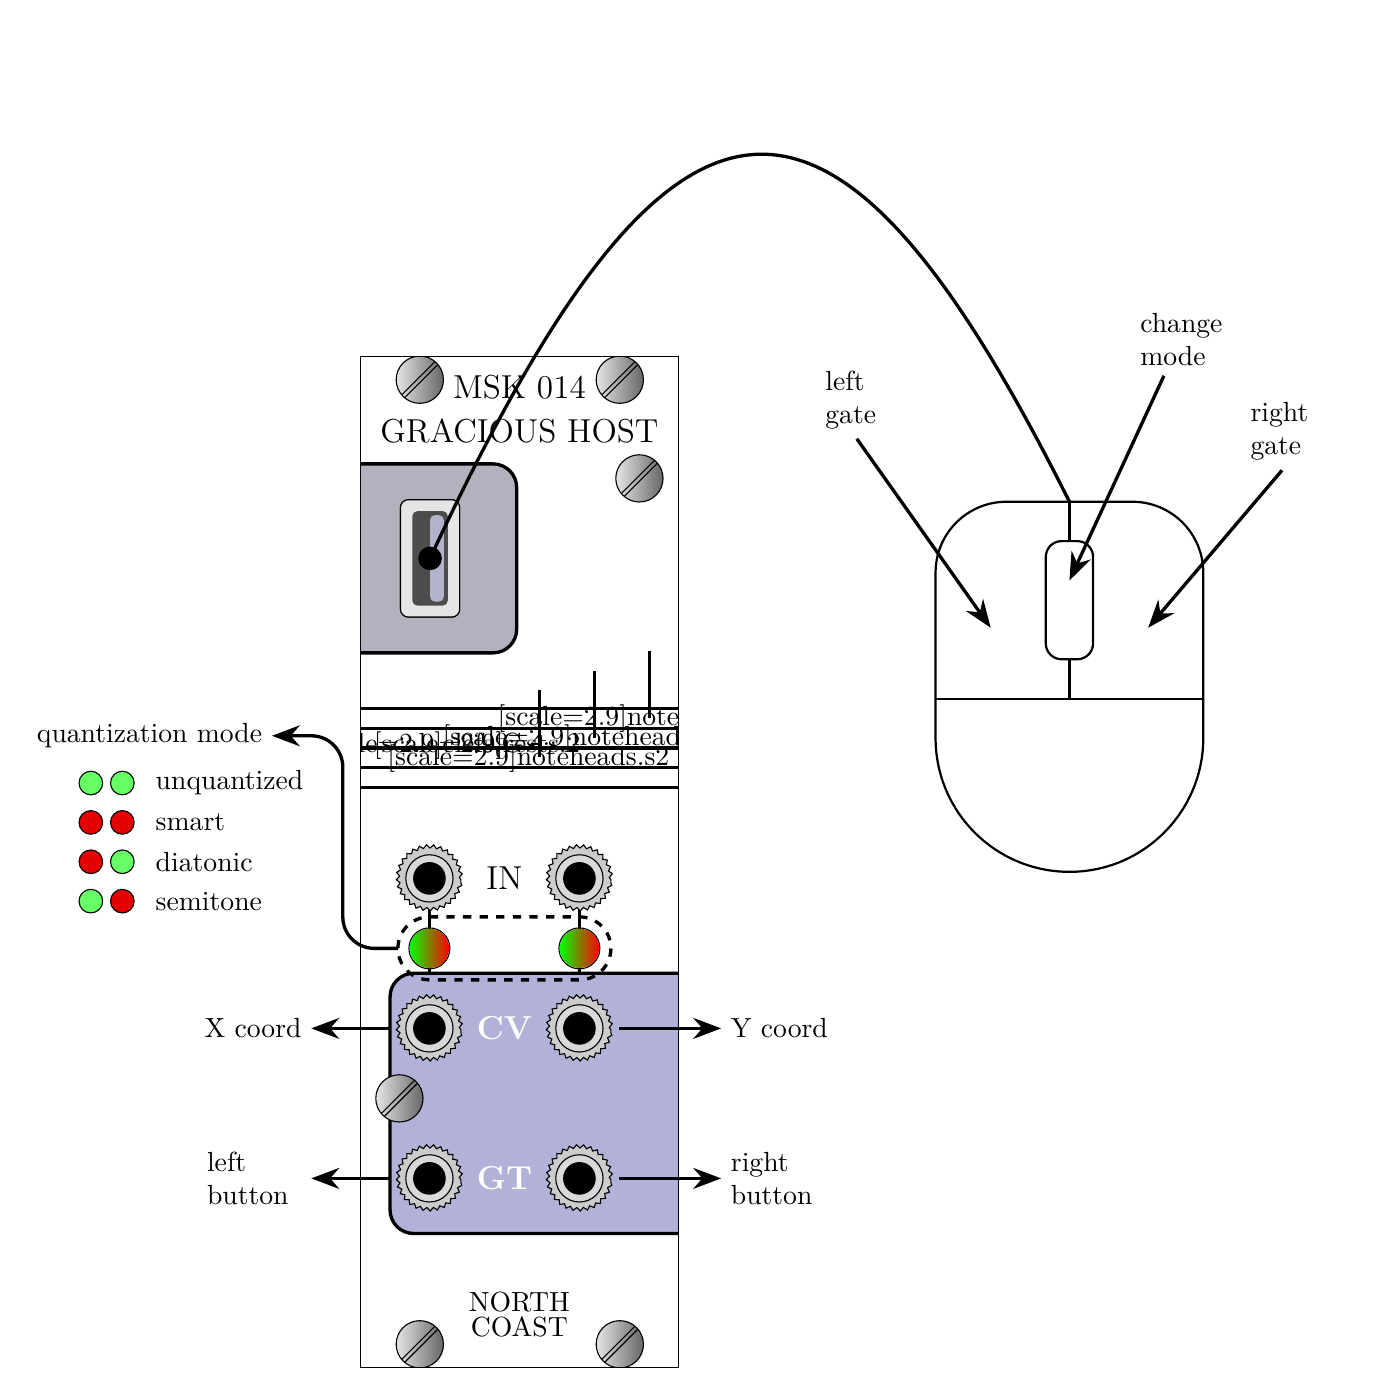
\begin{tikzpicture}
  \begin{scope}
    \setmainfont[Path={../../tsukurimashou/otf/},
      BoldFont={TsukurimashouBokukkoExtraBoldPS}]{TsukurimashouBokukkoDemiboldPS}%
    % start out defining coordinates
    \coordinate (o) at (0,0);
    \coordinate (llrh) at ($(o)+(7.50mm,3.00mm)$) {};
    \coordinate (ulrh) at ($(o)+(7.50mm,125.50mm)$) {};
    \coordinate (lrrh) at ($(o)+(32.90mm,3.00mm)$) {};
    \coordinate (urrh) at ($(o)+(32.90mm,125.50mm)$) {};
    \coordinate (lbh) at ($(o)+(4.91mm,34.23mm)$) {};
    \coordinate (ubh) at ($(o)+(35.39mm,112.97mm)$) {};
    \coordinate (j1) at ($(o)+(8.72mm,62.17mm)$) {};
    \coordinate (j2) at ($(o)+(27.77mm,62.17mm)$) {};
    \coordinate (j3) at ($(o)+(8.72mm,43.12mm)$) {};
    \coordinate (j4) at ($(o)+(27.77mm,43.12mm)$) {};
    \coordinate (j5) at ($(o)+(8.72mm,24.07mm)$) {};
    \coordinate (j6) at ($(o)+(27.77mm,24.07mm)$) {};
    \coordinate (d5) at ($(o)+(8.72mm,53.28mm)$) {};
    \coordinate (d6) at ($(o)+(27.77mm,53.28mm)$) {};
    \coordinate (j11) at ($(o)+(8.80mm,102.81mm)$) {};
%
    \coordinate (cpn) at ($(o)+(20.15mm,128.50mm)$) {};
    \coordinate (cps) at ($(o)+(20.15mm,0mm)$) {};
    \coordinate (cpe) at ($(o)+(40.30mm,64.25mm)$) {};
    \coordinate (cpw) at ($(o)+(0mm,64.25mm)$) {};
%
    % background
    \draw[fill=white] (o) rectangle (40.30mm,128.50mm);
    \clip (o) rectangle (40.30mm,128.50mm);
  %
    \draw[very thick,black,fill=blue!15!black!30!white,rounded corners=3.0mm]
      ($(j11)+(-15mm,-12mm)$) rectangle ($(j11)+(11mm,12mm)$);
    \draw[very thick,black] (j1) -- (j3);
    \draw[very thick,black] (j2) -- (j4);
    \draw[very thick,black,fill=blue!50!black!30!white,rounded corners=3.0mm]
      ($(j5)+(-5mm,-7mm)$) rectangle ($(j4-|cpe)+(5mm,7mm)$);
    \node at ($(j1)!0.5!(j2)$) {\large IN};
    \node[white] at ($(j3)!0.5!(j4)$) {\large\textbf{CV}};
    \node[white] at ($(j5)!0.5!(j6)$) {\large\textbf{GT}};
  %
    \coordinate (sref) at ($(j1)!0.53!(j11)$) {};
    \coordinate (nref) at ($(sref)+(9.525mm,-20.32mm)$) {};
    \draw[very thick] ($(sref-|cpw)$)
      -- ($(sref-|cpe)$);
    \draw[very thick] ($(sref-|cpw)+(0,-2.5mm)$)
      -- ($(sref-|cpe)+(0,-2.5mm)$);
    \draw[very thick] ($(sref-|cpw)+(0,-5mm)$)
      -- ($(sref-|cpe)+(0,-5mm)$);
    \draw[very thick] ($(sref-|cpw)+(0,-7.5mm)$)
      -- ($(sref-|cpe)+(0,-7.5mm)$);
    \draw[very thick] ($(sref-|cpw)+(0,-10mm)$)
      -- ($(sref-|cpe)+(0,-10mm)$);
    \node at ($(nref)+(-11.0mm,15.62mm)$)
      {\lilyGlyph[scale=2.9]{clefs.G}};
    \node at ($(nref)+(-3.5mm,15.62mm)$)
      {\lilyGlyph[scale=2.9]{rests.2}};
    \foreach \x/\y in {3.00/0.05,10.00/2.55,17.00/5.05} {
      \node at ($(nref)+(\x mm,14mm+\y mm)$)
        {\lilyGlyph[scale=2.9]{noteheads.s2}};
      \draw[very thick]
        ($(nref)+(\x mm+1.4mm,14.1mm+\y mm)$) -- ++(0,8.5mm);
    }
  %
    \node at ($(cpn)+(0.0mm,-4.0mm)$) {\large MSK 014};
    \node at ($(cpn)+(0.0mm,-9.5mm)$) {\large GRACIOUS HOST};
    \node at ($(cps)+(0.0mm,8.5mm)$)
      {\parbox{0.9in}{\linespread{0.75}\selectfont\center NORTH COAST}};
%
    % panel-to-rails mounting holes, 3.2mm holes to clear M3 machine screw
    \draw (llrh) circle[radius=1.60mm];
    \draw (ulrh) circle[radius=1.60mm];
    \draw (lrrh) circle[radius=1.60mm];
    \draw (urrh) circle[radius=1.60mm];
    % board-to-panel mounting holes, to clear M3 machine screw
    \draw (lbh) circle[radius=1.60mm];
    \draw (ubh) circle[radius=1.60mm];
    % six jacks with M6 threads, 6.3mm holes
    \draw (j1) circle[radius=3.15mm];
    \draw (j2) circle[radius=3.15mm];
    \draw (j3) circle[radius=3.15mm];
    \draw (j4) circle[radius=3.15mm];
    \draw (j5) circle[radius=3.15mm];
    \draw (j6) circle[radius=3.15mm];
    % two LEDs, 5.20mm holes
    \draw (d5) circle[radius=2.60mm];
    \draw (d6) circle[radius=2.60mm];
    % rectangular hole for USB A connector
    \draw[rounded corners=1mm]
      ($(j11)+(-3.76mm,-7.45mm)$) rectangle ($(j11)+(3.76mm,7.45mm)$);
%
    % machine screws with 6mm heads
    \foreach \screwname in {llrh,ulrh,lrrh,urrh,lbh,ubh} {
      \path[draw=black,shading=ball,
        left color=black!10!white,right color=black!60!white]
        (\screwname) circle[radius=3mm];
      \draw ($(\screwname)+(50:3.0mm)$)--($(\screwname)+(220:3.0mm)$);
      \draw ($(\screwname)+(40:3.0mm)$)--($(\screwname)+(230:3.0mm)$);
    }
    % jacks with knurled nuts
    \foreach \jackname in {j1,j2,j3,j4,j5,j6} {
      \path[draw=black,fill=black!20!white,
        decorate,decoration={snake,amplitude=0.6,segment length=2.5}]
        ($(\jackname)+(0,-0.15mm)$) circle[radius=4mm];
      \path[draw=black,fill=black!15!white] (\jackname) circle[radius=3mm];
      \path[draw=black,fill=black] (\jackname) circle[radius=2mm];
    }
    % LEDs with red/green gradient
    \foreach \ledname in {d5,d6} {
      \path[shading=ball,left color=green,right color=red]
        (\ledname) circle[radius=2.50mm];
    }
    % mock up USB connector
    \draw[rounded corners=1mm,fill=black!10!white]
      ($(j11)+(-3.76mm,-7.45mm)$) rectangle ($(j11)+(3.76mm,7.45mm)$);
    \fill[rounded corners=0.64mm,fill=black!70!white]
      ($(j11)+(-2.25mm,-6.00mm)$) rectangle ($(j11)+(2.25mm,6.00mm)$);
    \fill[rounded corners=0.64mm,fill=blue!35!black!30!white]
      ($(j11)+(0,-5.50mm)$) rectangle ($(j11)+(1.75mm,5.50mm)$);
  \end{scope}
  \draw (o) rectangle (40.30mm,128.50mm);
%
  \coordinate (mtab) at ($(d5)+(-20mm,27mm)$) {};
  \draw[very thick,{Stealth[scale=1.2]}-,rounded corners=4mm]
    (mtab) -- ($(d5|-mtab)+(-11mm,0mm)$) --
    ($(d5)+(-11mm,0)$) -- ($(d5)+(-4mm,0)$);
  \draw[rounded corners=4mm,very thick,dashed]
    ($(d5)+(-4mm,-4mm)$) rectangle ($(d6)+(4mm,4mm)$);
  \draw[very thick,{Stealth[scale=1.2]}-]
    ($(j3)+(-15mm,0)$) -- ($(j3)+(-5mm,0)$);
  \draw[very thick,{Stealth[scale=1.2]}-]
    ($(j4)+(18mm,0)$) -- ($(j4)+(5mm,0)$);
  \draw[very thick,{Stealth[scale=1.2]}-]
    ($(j5)+(-15mm,0)$) -- ($(j5)+(-5mm,0)$);
  \draw[very thick,{Stealth[scale=1.2]}-]
    ($(j6)+(18mm,0)$) -- ($(j6)+(5mm,0)$);
%
  \node[anchor=east] at (mtab) {quantization mode};
  \node[anchor=east] at ($(j3)+(-15mm,0)$) {X coord};
  \node[anchor=west] at ($(j4)+(18mm,0)$) {Y coord};
  \node[anchor=east] at ($(j5)+(-15mm,0)$)
    {\parbox{12mm}{left button}};
  \node[anchor=west] at ($(j6)+(18mm,0)$)
    {\parbox{12mm}{right button}};
%
  \path[draw,fill=green!60!white] ($(mtab)+(-23mm,-6mm)$)
    circle[radius=1.50mm];
  \path[draw,fill=green!60!white] ($(mtab)+(-19mm,-6mm)$)
    circle[radius=1.50mm];
  \node[anchor=west] at ($(mtab)+(-16mm,-6mm)$)
    {unquantized};
%
  \path[draw,fill=red!90!black] ($(mtab)+(-23mm,-11mm)$)
    circle[radius=1.50mm];
  \path[draw,fill=red!90!black] ($(mtab)+(-19mm,-11mm)$)
    circle[radius=1.50mm];
  \node[anchor=west] at ($(mtab)+(-16mm,-11mm)$)
    {smart};
%
  \path[draw,fill=red!90!black] ($(mtab)+(-23mm,-16mm)$)
    circle[radius=1.50mm];
  \path[draw,fill=green!60!white] ($(mtab)+(-19mm,-16mm)$)
    circle[radius=1.50mm];
  \node[anchor=west] at ($(mtab)+(-16mm,-16mm)$)
    {diatonic};
%
  \path[draw,fill=green!60!white] ($(mtab)+(-23mm,-21mm)$)
    circle[radius=1.50mm];
  \path[draw,fill=red!90!black] ($(mtab)+(-19mm,-21mm)$)
    circle[radius=1.50mm];
  \node[anchor=west] at ($(mtab)+(-16mm,-21mm)$)
    {semitone};
%
  \coordinate (mouse) at ($(o)+(90mm,110mm)$) {};
  \coordinate (arctop) at ($(o)+(50mm,170mm)$) {};
  \fill (j11) circle[radius=1.50mm];
  \draw[very thick] (j11)
    ..controls ($(arctop)+(-10mm,0)$) and ($(arctop)+(10mm,0)$)..
    (mouse);
  \path[thick,draw,fill=white]
    ($(mouse)+(-17mm,-9mm)$)
      arc[start angle=180,end angle=90,radius=9mm] --
    ($(mouse)+(-8mm,0mm)$) -- ($(mouse)+(8mm,0mm)$)
      arc[start angle=90,end angle=0,radius=9mm] --
    ($(mouse)+(17mm,-30mm)$)
      arc[start angle=0,end angle=-180,radius=17mm]
    --cycle;
  \draw[thick] ($(mouse)+(-17mm,-25mm)$) -- ($(mouse)+(17mm,-25mm)$);
  \draw[thick] (mouse) -- ($(mouse)+(0mm,-25mm)$);
  \draw[thick,fill=white,rounded corners=2mm]
    ($(mouse)+(-3mm,-20mm)$) rectangle ($(mouse)+(3mm,-5mm)$);
%
  \draw[very thick,{Stealth[scale=1.2]}-]
    ($(mouse)+(-10mm,-16mm)$) -- ($(mouse)+(-27mm,8mm)$);
  \draw[very thick,{Stealth[scale=1.2]}-]
    ($(mouse)+(10mm,-16mm)$) -- ($(mouse)+(27mm,4mm)$);
  \draw[very thick,{Stealth[scale=1.2]}-]
    ($(mouse)+(0mm,-10mm)$) -- ($(mouse)+(12mm,16mm)$);
%
  \node[anchor=south] at ($(mouse)+(-25mm,8mm)$) {\parbox{12mm}{left gate}};
  \node[anchor=south] at ($(mouse)+(29mm,4mm)$) {\parbox{12mm}{right gate}};
  \node[anchor=south] at ($(mouse)+(15mm,16mm)$) {\parbox{12mm}{change mode}};
\end{tikzpicture}\par}
\caption{Mouse interface functions.}\label{fig:mouse-conn}
\end{figure*}

The standardization of USB mice is much like that of typing keyboards:  the
relevant standard includes a very complicated protocol and a simple one, and
most implementors only use the simple one.  In technical terms, the Gracious
Host supports the ``boot mouse'' protocol, for USB devices that expose an
interface descriptor of class 3, subclass 1, protocol 2.  Nearly all
commonly-available USB mice can operate under this protocol.

The basic function with a mouse attached is that the left and right mouse
buttons send gates (to the Gracious Host's digital outputs) and the X and Y
coordinates of mouse motion control the analog CV outputs.  The middle
button (or wheel, when clicked) cycles between the quantization modes below;
and the colours of the LEDs (which light up on button presses) indicate the
current mode.

\begin{itemize}
  \item Unquantized (both LEDs green; default on startup) -- CV outputs
    directly reflect the current X and Y coordinates.
  \item Smart quantize (both LEDs red) -- CV outputs are quantized to a
    diatonic scale that attempts to automatically follow the notes you play. 
    Play the fourth of the (major) scale three times without playing the
    seventh and it will shift to the subdominant key; play the seventh three
    times without playing the fourth, and it will shift to the dominant.  In
    practice, this allows for free improvisation with the somewhat clumsy
    mouse control, while keeping everything more or less sounding like it is
    in tune.
  \item Quantize to fixed scale (left LED red, right green) -- CV outputs
    are quantized to a fixed diatonic scale (C major or A minor, if 0V
    output is considered to be C).
  \item Quantize to semitones (left LED green, right red) -- CV outputs are
    quantized to V/oct semitones, that is, round multiples of $1/12$ of a
    volt.
\end{itemize}

In the quantization modes, the CVs are quantized only while the button is
held and the gate is high; otherwise they are unquantized.  That way, it is
convenient to build a patch where one voltage is quantized pitch and the
other is something like filter cutoff not meant to be quantized; to control
the patch as intended, just don't press the button on the unquantized side.

The input jacks are not used in mouse mode, and (because the USB boot mouse
protocol does not specify this) the mouse wheel's scrolling
function, other than clicking it, has no consistent interpretation.

% $Id: warnings.tex 5678 2017-10-13 15:20:20Z mskala $

%
% MSK 010 safety and other warnings
% Copyright (C) 2017  Matthew Skala
%
% This program is free software: you can redistribute it and/or modify
% it under the terms of the GNU General Public License as published by
% the Free Software Foundation, version 3.
%
% This program is distributed in the hope that it will be useful,
% but WITHOUT ANY WARRANTY; without even the implied warranty of
% MERCHANTABILITY or FITNESS FOR A PARTICULAR PURPOSE.  See the
% GNU General Public License for more details.
%
% You should have received a copy of the GNU General Public License
% along with this program.  If not, see <http://www.gnu.org/licenses/>.
%
% Matthew Skala
% https://northcoastsynthesis.com/
% mskala@northcoastsynthesis.com
%

\chapter{Safety and other warnings}

Ask an adult to help you.

North Coast Synthesis Ltd.\ does not offer warranties or technical support
on anything we did not build and sell.  That applies both to modules built
by you or others from the kits we sell, and to fully-assembled modules that
might be built by others using our plans.  Especially note that because we
publish detailed plans and we permit third parties to build and sell modules
using our plans subject to the relevant license terms, it is reasonable to
expect that there will be modules on the new and used markets closely
resembling ours but not built and sold by us.  We may be able to help in
authenticating a module of unknown provenance; contact us if you have
questions of this nature.

For new modules purchased through a reseller, warranty and technical support
issues should be taken to the reseller \emph{first}.  Resellers buy modules
from North Coast at a significant discount, allowing them to resell the
modules at a profit, and part of the way they earn that is by taking
responsibility for supporting their own customers.

We also sell our products to hobbyists who enjoy tinkering with and
customizing electronic equipment.  Modules like ours, even if originally
built by us, may be quite likely to contain third-party ``mods,'' added or
deleted features, or otherwise differ from the standard specifications of
our assembled modules when new.  Be aware of this possibility when you buy a
used module.

Soldering irons are very hot.

Solder splashes and cut-off bits of component leads can fly a greater
distance and are harder to clean up than you might expect.  Spread out some
newspapers or similar to catch them, and wear eye protection.

Lead solder is toxic, as are some fluxes used with lead-free solder.  Do not
eat, drink, smoke, pick your nose, or engage in sexual activity while using
solder, and wash your hands when you are done using it.

Solder flux fumes are toxic, \emph{especially} from lead-free solder
because of its higher working temperature.  Use appropriate ventilation.

Some lead-free solder alloys produce joints that look ``cold''
(i.e.\ defective) even when they are correctly made.  This effect can be
especially distressing to those of us who learned soldering with lead solder
and then switched to lead-free.  Learn the behaviour of whatever alloy you  
are using, and then trust your skills.

Water-soluble solder flux must be washed off promptly (within less than an
hour of application) because if left in place it will corrode the metal. 
Solder with water-soluble flux should not be used with stranded wire because
it is nearly impossible to remove from between the strands.

Residue from traditional rosin-based solder flux can result in undesired
leakage currents that may affect high-impedance circuits, and this module
uses impedances into the megaohm range, where the leakage currents may have
some effect on circuit operation.  If your soldering leaves a lot of such
residue then it might be advisable to clean that off.

Voltage and current levels in some synthesizer circuits may be dangerous.

Building your own electronic equipment is seldom cheaper than buying
equivalent commercial products, due to commercial economies of scale from
which you as small-scale home builder cannot benefit.  If you think getting
into DIY construction is a way to save money, you will probably be
disappointed.

% $Id: bom.tex 9376 2021-08-31 13:12:43Z mskala $

%
% MSK 008 bill of materials
% Copyright (C) 2017  Matthew Skala
%
% This program is free software: you can redistribute it and/or modify
% it under the terms of the GNU General Public License as published by
% the Free Software Foundation, version 3.
%
% This program is distributed in the hope that it will be useful,
% but WITHOUT ANY WARRANTY; without even the implied warranty of
% MERCHANTABILITY or FITNESS FOR A PARTICULAR PURPOSE.  See the
% GNU General Public License for more details.
%
% You should have received a copy of the GNU General Public License
% along with this program.  If not, see <http://www.gnu.org/licenses/>.
%
% Matthew Skala
% https://northcoastsynthesis.com/
% mskala@northcoastsynthesis.com
%

\onecolumn
\chapter{Bill of materials}

{\centering
\fbox{This table is not a substitute for the text instructions.}

\begin{longtable}{rp{1.3in}cp{3in}}
  \textbf{Qty} & \textbf{Ref} & \textbf{Value/Part No.} & \\ \hline \endhead
\input{bomdata.tex}
\end{longtable}\par}

Not listed above, but also needed:  front panel, two circuit boards,
three 14-pin DIP sockets, solder, etc.
Fixed resistors should be 1\%\ metal film, except those specified as 0.1\%. 
North Coast Synthesis Ltd.\ kits or assembled modules sometimes contain
other parts with equivalent or better specifications rather than exact
manufacturers and part numbers shown here.

\twocolumn

% $Id: board2.tex 9464 2021-10-14 16:51:12Z mskala $

%
% MSK 009 Board 2 build instructions
% Copyright (C) 2018  Matthew Skala
%
% This program is free software: you can redistribute it and/or modify
% it under the terms of the GNU General Public License as published by
% the Free Software Foundation, version 3.
%
% This program is distributed in the hope that it will be useful,
% but WITHOUT ANY WARRANTY; without even the implied warranty of
% MERCHANTABILITY or FITNESS FOR A PARTICULAR PURPOSE.  See the
% GNU General Public License for more details.
%
% You should have received a copy of the GNU General Public License
% along with this program.  If not, see <http://www.gnu.org/licenses/>.
%
% Matthew Skala
% https://northcoastsynthesis.com/
% mskala@northcoastsynthesis.com
%

\chapter{Building Board 2}

The recommended order for building this module is to assemble Board 2, the
one further from the front panel, first.  That will make it easier to get
all the physical positioning right for the components that bridge between
the boards or pass through the panel.

Note that although I'm describing a separate step for each component value,
and that's how I built my prototype so as to have plenty of photo
opportunities, if you are reasonably confident about your skills you may
find it easier to populate all or most of the board (i.e.\ put the
components in place) and then solder them in a single step.  Except where
noted, the order in which you add components does not matter much.

\section{Preliminaries}

Count out the right number of everything according to the bill of materials. 
There is an abbreviated BOM for Board~2, excluding a few items that will be
added when combining this board with Board~1, in Table~\ref{tab:b2bom}.

\nopagebreak
\noindent\includegraphics[width=\linewidth]{board2-parts.jpg}

There are two trimmers to be installed on this board.  Before
installing them, use an ohmmeter to adjust each one to 50\% of its range. 
Measure the resistance along the track, then measure the resistance from the
wiper to one end and adjust to make the wiper half the total track
resistance.  This need not be exact, but having them start near their
midpoints will help with adjustment later,
by reducing issues with interaction among the different settings.  With both
trimmers pre-set to 50\%, the module should basically work even if it is not
at its best, whereas if they are installed at extreme values instead, then
you may have trouble getting it up and running enough to adjust it more
accurately.

\begin{table*}
{\centering
\fbox{This table is not a substitute for the text instructions.}
\vspace{\baselineskip}

\begin{tabular}{rp{1.3in}cp{3in}}
  \textbf{Qty} & \textbf{Ref} & \textbf{Value/Part No.} & \\ \hline
\input{bomdata-2.tex}
\end{tabular}\par}
\caption{Bill of Materials for assembling Board~2.  Also needed is the PCB
itself.}\label{tab:b2bom}
\end{table*}

\section{Decoupling capacitors}

The four axial ceramic 0.1$\mu$F decoupling capacitors, C8 to C11, are shown
on the board by a special symbol without their reference designators.

\nopagebreak
\noindent\includegraphics[width=\linewidth]{decoup-symbol.jpg}

Install these four capacitors where the symbol appears.  They are not
polarized and may be installed in either orientation.  These capacitors act
as filters for the power supplies to the op amp and OTA chips.  An MSK~009
kit should include six of these capacitors, and only four are used on this
board; save the remaining two for use on Board~1.

\nopagebreak
\noindent\includegraphics[width=\linewidth]{{cap-0.1u2}.jpg}

\section{Fixed resistors}

Resistors are never polarized.  I like to install mine in a consistent
direction for cosmetic reasons, but this is electrically unnecessary.  In
this module, the fixed resistors are metal film 1\%\ type.  They usually
have blue bodies and four colour bands designating the value, plus a fifth
band for the tolerance.  The tolerance band is brown for 1\%, but note that
we may occasionally ship better-tolerance resistors in the kits than the
specifications require, if we are able to source them at a good price. 
Accordingly, I mention only the four value band colours for this type of
resistor; if you are using resistors with other codes, you are responsible
for knowing them.  Note that colour codes on metal film 1\% resistors are
often ambiguous (reading from one end or the other end may give two
different values, both plausible) and some of the colours are hard to
distinguish anyway.  If in doubt, always measure with an ohmmeter before
soldering the resistor in place.

Install the four 510$\Omega$ (green-brown-black-black) resistors R22, R23,
R32, and R33.  These resistors, with the 100k$\Omega$ ones added later, set
the signal levels at the inputs of the OTA chips.

\nopagebreak
\noindent\includegraphics[width=\linewidth]{{res-510}.jpg}

\pagebreak
Install the two 9.1k$\Omega$ (white-brown-black-brown) resistors R24 and
R34.  These limit the maximum control current for the OTAs.

\nopagebreak
\noindent\includegraphics[width=\linewidth]{{res-9.1k}.jpg}

Install the two 10k$\Omega$ (brown-black-black-red) resistors R25 and R35. 
These are feedback resistors for the current-to-voltage converters in the
filter core.

\nopagebreak
\noindent\includegraphics[width=\linewidth]{{res-10k}.jpg}

\pagebreak
Install the four 27k$\Omega$ (red-violet-black-red) resistors R21, R26, R31, and R36. 
These are feedback resistors for the integrators (R26 and R36), and set the
current for the linearizing diodes in the LM13700 chips (R1 and R31).

\nopagebreak
\noindent\includegraphics[width=\linewidth]{{res-27k}.jpg}

Install the two 100k$\Omega$ (brown-black-black-orange) resistors R18 and
R28.  These resistors participate in setting the input levels for the OTA
chips.  A full kit contains seven resistors of this value; five should
remain for use on Board~1.

\nopagebreak
\noindent\includegraphics[width=\linewidth]{{res-100k2}.jpg}

Install the two 220k$\Omega$ (red-red-black-orange) resistors R19 and
R29.  These resistors set the adjustment ranges for the DC offset trimmers.
A full kit contains four
resistors of this value; save two for use on Board~1.

\nopagebreak
\noindent\includegraphics[width=\linewidth]{{res-220k2}.jpg}

\section{Semiconductors}

Install the two 1N5818 or SBA130 Schottky rectifier diodes D2 and D3.  These
are for reverse-voltage protection; they cut off power to the module when
the power plug is backwards.  They are polarized and it is important to
install them in the right direction.  Each diode is packaged inside a black
or dark grey plastic slug with a white or light grey stripe at one end; that
end is the \emph{cathode}.  The silkscreen markings on the board have a
corresponding stripe and the diodes should be installed with their stripes
matching the markings on the board.  The solder pads for the cathodes are
also square instead of round.  Installing these backwards means they will
have the opposite of the intended protective effect.

\nopagebreak
\noindent\includegraphics[width=\linewidth]{schottky.jpg}

Install the 14-pin DIP socket for the operational amplifier chip U2.  This
chip does most of the amplification in the filter core.  DIP sockets
themselves do not care which direction you install them, but it is
critically important that the chips installed in the sockets should be
installed in the right direction.  To help with that, the sockets will
probably be marked with notches at one end (indicating the end where Pin~1
and Pin~14 are located) and you should install the sockets so that the
notched ends match the notches shown on the PCB silkscreen.  The solder pad
for Pin~1 is also distinguished by being rectangular instead of rounded.

Installing DIP sockets without having them tilted at a funny angle can be
tricky.  I recommend inserting the socket in the board, taping it in place
on the component side with vinyl electrical tape or sticking it there with a
small blob of putty at each end, then soldering one pin on
one corner and checking that the socket is snug against the board before
soldering the other pins.  That way, if you accidentally solder the first
pin with the socket tilted, it will be easier to correct (only one pin to
desolder instead of all of them).

\nopagebreak
\noindent\includegraphics[width=\linewidth]{dip14-2.jpg}

If you somehow manage to solder an entire socket in backwards, don't try to
desolder it to turn it around.  Just leave it as it is and remember that
when you insert the chip, you must insert it so the chip matches the
markings on the \emph{board}, not the turned-around socket.

Install the 16-pin DIP socket for the OTA (operational transconductance
amplifier) chip U3.  This chip contains two current-controlled amplifiers,
which, by means of a frequency-dependent control current, tune the filter
core to the desired frequency.  See the general instructions regarding DIP
sockets above.

\nopagebreak
\noindent\includegraphics[width=\linewidth]{dip16.jpg}

\section{Electrolytic and film capacitors}

Install the two 6800pF film capacitors C2 and C3.  These are timing
components used in the integrators at low frequencies to complement the
inductors used at medium to high frequencies.  They are unpolarized
components and may be installed in either orientation.

The markings on film capacitors may vary depending on the manufacturer and
model.  These ones might be marked ``682'' (for 68 followed by two 0s number
of picofarads), ``6n8'' (for 6.8nF), or even ``0.0068'' (value in $\mu$F). 
However, these are the only film capacitors in the module, so confusion is
unlikely.

\nopagebreak
\noindent\includegraphics[width=\linewidth]{{cap-6800p}.jpg}

\pagebreak

Install the two 10$\mu$F electrolytic capacitors C4 and C5, which
filter the power supply for the module as a whole. 
These are polarized components and they may explode if installed backwards. 
Each one will be marked on its casing with a stripe and minus signs to
indicate the negative lead; the positive lead will probably also be longer. 
These clues should be matched with the markings on the PCB: plus and minus
symbols in the silkscreen and a square solder pad for the positive (long)
lead.

\nopagebreak
\noindent\includegraphics[width=\linewidth]{cap-10u.jpg}

\section{Trimmer potentiometers}

If you have not already set the trimmers to 50\%\ of their full scale value
as described under ``Preliminaries'' above, then do it now.

Trimmers usually are not washable, so if you plan to clean your boards by
full immersion in water or other solvent,
your last chance is now; future cleaning will have to
be done with a brush and some care to avoid letting liquid seep into the
trimmers.  Even now you should take some care with the DIP sockets, because
solvent can carry flux residue into them and form a varnish-like layer if
not carefully rinsed away.

Trimmers are not exactly polarized, but the three legs of each trimmer serve
different functions and need to be connected to the right holes.  The
physical arrangement of the legs and corresponding holes should make it
impossible to install the trimmers wrong way round.

Install the two 100k$\Omega$ trimmers R20 and R30.  These trimmers
are for compensating DC offsets in the filter core.

\nopagebreak
\noindent\includegraphics[width=\linewidth]{pot-100k2.jpg}

\pagebreak

\section{Inductors}

The two 22mH ferrite-bobbin inductors, that is, \emph{coils}, L1 and L2 give
this module its name.  Install them now.  They are the main timing
components in the filter core, serving at medium to high frequencies. 
Single inductors like these have no polarity and may be installed in either
direction; the situation is more complicated with transformers made of two
or more interacting inductors.

The inductors are delicate, especially in the area where the leads attach to
the bodies, because the windings that connect to the leads are made of very
fine wire.  The ferrite core material is also somewhat brittile.  It is
important not to bend the leads too close to the bodies.  There is some
extra space for the inductors on the circuit board to allow for a gentle
bend radius.

\nopagebreak
\noindent\includegraphics[width=\linewidth]{coils.jpg}

\section{Eurorack power connector}

Install the 2$\times$5-pin Eurorack power connector J2.  This connector is
not polarized in itself, although the connection it makes is polarized.  As
with the DIP sockets, you should be careful to get it installed snugly
against the board, not tilted at an angle.  Use tape or putty to
hold it in place, solder one pin, then check that it is straight before you
solder the other pins.

The six pins in the centre of the connector, that is all except the four
corner pins, are for grounding and they are all connected together on the
board.  Thus, if you accidentally form solder bridges among these six pins
while installing the connector, don't waste effort trying to remove them;
they will have no electrical effect.

\nopagebreak
\noindent\includegraphics[width=\linewidth]{power.jpg}

In between completed boards is a good time to take a break.


% $Id: board1.tex 9376 2021-08-31 13:12:43Z mskala $

%
% MSK 008 Board 1 build instructions
% Copyright (C) 2017, 2018  Matthew Skala
%
% This program is free software: you can redistribute it and/or modify
% it under the terms of the GNU General Public License as published by
% the Free Software Foundation, version 3.
%
% This program is distributed in the hope that it will be useful,
% but WITHOUT ANY WARRANTY; without even the implied warranty of
% MERCHANTABILITY or FITNESS FOR A PARTICULAR PURPOSE.  See the
% GNU General Public License for more details.
%
% You should have received a copy of the GNU General Public License
% along with this program.  If not, see <http://www.gnu.org/licenses/>.
%
% Matthew Skala
% https://northcoastsynthesis.com/
% mskala@northcoastsynthesis.com
%

\chapter{Building Board 1}\label{ch:board1}

Board~1 has components on both sides, and for best results, it is important
to install them in the right order.  Build Board~2 first, and see the
general comments in the Board~2 chapters about how to approach the task.

\section{Preliminaries}

Count out the right number of everything according to the bill of materials. 
There is an abbreviated BOM for the items needed in this chapter (including
the final assembly of the module) in Table~\ref{tab:b1bom}.  It
is also assumed you have a finished Board~2 from the previous chapter.

\noindent\includegraphics[width=\linewidth]{board1-parts.jpg}

\begin{table*}
{\centering
\fbox{This table is not a substitute for the text instructions.}
\vspace{\baselineskip}

\begin{tabular}{rp{1.3in}cp{3in}}
  \textbf{Qty} & \textbf{Ref} & \textbf{Value/Part No.} & \\ \hline
\input{bomdata-1.tex}
\end{tabular}\par}
\caption{Bill of Materials for Board~1.}\label{tab:b1bom}
\end{table*}

If you wish to reconfigure the CV2 inputs, you can change the solder jumpers
on Board~1 at this point.  In a standard build, the CV2 input on the left
channel \emph{adds} its voltage to CV1 and the quantizer output, while the
CV2 input on the right channel \emph{subtracts}.  This configuration is the
most useful one for most users and it is not particularly recommended to
change it.  But if you want to, first locate the jumpers on the board.  JP1
on the left is for the left channel and JP2 on the right is for the right
channel.

\noindent\includegraphics[width=\linewidth]{jumpers.jpg}

Each jumper has three terminals.  The middle one is connected to the one on
the left or the right for positive (adding) or negative (subtracting)
respectively, with a default set by a trace built into the circuit board. 
To change the jumper, use a sharp knife to carefully cut the connecting
trace, and then apply a blob of solder connecting the middle terminal to the
one for the opposite selection.  Use an ohmmeter to check that you have
really broken the connection on one side and recreated it on the other.

For a more advanced modification, you can solder fine wires into the holes
provided and run them into other circuitry of your own construction.  If you
add an SPDT switch, you could use it to change the add/subtract option by
flipping the switch.  You could also connect any number of additional
inverting and noninverting input jacks through 100k$\Omega$ precision
resistors (0.1\%\ or better) to the $+$ and $-$ terminals, which as shown on
the schematic diagram are op amp virtual ground summing nodes.

\section{Decoupling capacitors}

The two axial ceramic 0.1$\mu$F decoupling capacitors C7 and C8 are shown on
the board by a special symbol without their reference designators.

\noindent\includegraphics[width=\linewidth]{decoup-symbol.jpg}

\pagebreak

Install these two capacitors where the symbol appears.  They are not
polarized and may be installed in either orientation.  These capacitors act
as filters for the power supplies to the op amp chip, protecting them from
high-frequency crosstalk.

\noindent\includegraphics[width=\linewidth]{{cap-0.1u1}.jpg}

\section{Fixed resistors}

Resistors are never polarized.  I like to install mine in a consistent
direction for cosmetic reasons, but this is electrically unnecessary.  In
this module, most resistors are metal film 1\%\ type; a few are 0.1\%\
precision metal film resistors.  Both kinds will usually have blue bodies
and four colour bands designating the value, plus a fifth band for the
tolerance, and these are the resistors shipped in the North Coast
kits.  The tolerance band is brown for 1\%\ and violet for 0.1\%, but note
that we may occasionally ship better-tolerance resistors in the kits than
the specifications require, if we are able to source them at a good price.
Accordingly, I mention only the four value band colours for this type of
resistor; if you are using resistors with other codes, you are responsible
for knowing them.  Note that colour codes on metal film 1\% resistors are
often ambiguous (reading from one end or the other end may give two
different values, both plausible) and some of the colours are hard to
distinguish anyway.  If in doubt, always measure with an ohmmeter before
soldering the resistor in place.

There are no cases in this module of the same nominal resistance value being
used at more than one tolerance, but the 0.1\%\ resistance values are marked
with asterisks (*) on the board silkscreen as a reminder that these
positions require special resistors.

The physical size of the resistors may vary, and details like the exact
colour of the bluish background.  You can see some of that variation in the
photos in these instructions.  Some of the resistance values used in this
module are hard to find, and we source different values from different
suppliers, so not all the resistors in a kit will necessarily be from the
same manufacturer, nor match on non-critical specifications like power
rating and physical size.

Install the four 910$\Omega$ (white-brown-black-black) resistors R50, R52,
R53, and R54.  These form part of the current-controlling network for the
LED drivers.

\noindent\includegraphics[width=\linewidth]{res-910.jpg}

Install the two 1k$\Omega$ (brown-black-black-brown) resistors R47 and R48. 
These are current-limiting resistors to protect external circuits from
excessive output power on the module outputs; they also serve to isolate the
op amp chip from reactive (capacitive or inductive) loads that could make it
unstable.  Do not confuse these resistors with other power-of-ten values
such as 100k$\Omega$, which also have codes starting brown-black-black but
with different colours for the fourth, exponent-indicating, colour band.

\noindent\includegraphics[width=\linewidth]{res-1k.jpg}

Install the two 1.2k$\Omega$ (brown-red-black-brown) resistors R49 and R51. 
These form part of the current-controlling network for the LED drivers.

\noindent\includegraphics[width=\linewidth]{{res-1.2k}.jpg}

\pagebreak

Install the two 75k$\Omega$ (violet-green-black-red) resistors R13 and R16. 
These set the weight of the quantizer voltage inputs in comparison to the
manual octave switches.

\noindent\includegraphics[width=\linewidth]{res-75k.jpg}

Install the two 1M$\Omega$ (brown-black-black-yellow) resistors R15 and R16. 
These set the weight of the manual octave switches in the quantizers.  Do
not confuse them with other power-of-ten resistance values.

\noindent\includegraphics[width=\linewidth]{res-1M.jpg}

Install the ten 100k$\Omega$ 0.1\%\ precision resistors.  These control the
gain of the summing and inversion op amp circuits.  When building the
prototypes I noticed that either these resistors are just a little larger
than others of the same approximate body size, or maybe their leads are a
little stiffer; I found that I needed to bend the leads tighter (closer to
the bodies) than usual in order to have them fit nicely on the board.  Take
it slowly and carefully.

\noindent\includegraphics[width=\linewidth]{res-100k.jpg}

\section{Semiconductors}

Install the four 1N4148 or 1N914 switching diodes D14, D16, D18, and D20,
and D19.  These switch the LED drive currents.
They are polarized components and it is important to
install them right way round.  Each diode is packaged inside a pink glass
bead with a black stripe at one end; that end is the \emph{cathode}.  The
silkscreen markings on the board have a corresponding stripe and the diodes
should be installed with their stripes matching the markings on the board. 
The solder pads for the cathodes are also square instead of round. 
Installing one or more of these diodes backwards will result in incorrect
operation of the LEDs.

\noindent\includegraphics[width=\linewidth]{diodes1.jpg}

Install the 14-pin DIP socket for the TL074B quad low-offset operational
amplifier (op amp) U5.  This chip processes the CV1 and CV2 inputs,
inverting them as necessary, and does the final summation to drive the
module output.  The socket itself does not care which direction you install
it, but it is critically important that the chip installed in the socket
should be installed in the right direction.  To help with that, the socket
will probably be marked with a notch at one end (indicating the end where
Pin~1 and Pin~14 are located) and you should install the socket so that the
notched end matches the notch shown on the PCB silkscreen.  The solder pad
for Pin~1 is also distinguished by being rectangular instead of rounded.

Two of the holes for the capacitors C5 and C6 are located just off one end
of the DIP socket's footprint at the same spacing, making it possible to
insert the DIP socket shifted over one space with two of its pins in the
capacitor holes.  Be careful not to do that.

Installing DIP sockets without having them tilted at a funny angle can be
tricky.  I recommend inserting the socket in the board, taping it in place
on the component side with vinyl electrical tape, then soldering one pin on
one corner and checking that the socket is snug against the board before
soldering the other pins.  That way, if you accidentally solder the first
pin with the socket tilted, it will be easier to correct (only one pin to
desolder instead of all of them).

\noindent\includegraphics[width=\linewidth]{dip1.jpg}

\section{Compensation capacitors}

Install the two 33pF radial ceramic capacitors C5 and C6.  They will
probably be marked ``330,'' which means 33pF in a scheme similar to the
resistor colour code:  significant digits 3 3 to be followed by 0 zeroes. 
These capacitors help ensure stability of the op amp drivers by killing the
frequency response at ultrasonic frequencies, making parasitic oscillation
harder to sustain.

\noindent\includegraphics[width=\linewidth]{cap-33p.jpg}

\section{Panel components}

Fasten the 10mm and 11mm standoffs to Board~1.  The 11mm standoffs
should be on the same side of the board as the resistors and other
components, with their male ends sticking up as shown; they will separate
the two boards when the module is fully assembled.  The 10mm standoffs
should be on the other side, where they will separate the circuit boards
from the panel, with their male ends through the holes in the board to mate
with the 11mm standoffs.  \emph{Do not confuse the two similar lengths of
standoffs.}  Arranging them wrong at this stage may result in soldering panel
components at the wrong spacing in a way that will eventually make it
impossible to assemble the module correctly.
There is an exploded diagram for the final module on
page~\pageref{fig:exploded}.  You may wish to consult it if the way the
hardware fits together is at all unclear.

\noindent\includegraphics[width=\linewidth]{standoffs.jpg}

\pagebreak

Place (do not solder yet) the LEDs D11 and D12 in their corresponding holes
on the board.  Single LEDs are polarized and can be destroyed by reverse
voltage.  These ones here are special bi-colour devices with two separate
LEDs in each package.  The internal connection is such that each one
protects the other from reverse voltage; so if connected backwards, they
will not be destroyed, but the intended green and red colours will be
swapped.  Each LED lens has one flat side, and one leg shorter than the
other on that side.  The short leg is Pin~1.  Its proper place on the board
is marked by a circle with a flattened side matching the direction of the
flattened side on the LED lens, and an oval solder pad.  The other leg
(Pin~2, long, farther from the flat side) goes into the rectangular solder
pad.  Be sure both LEDs are placed right way around according to these
clues.

\noindent\includegraphics[width=\linewidth]{led.jpg}

Place (do not solder yet) the eight jack sockets J1 to J8 in their
corresponding holes on the board.  Their arrangement of legs and
corresponding slotted holes is such that they will only fit one way.

\noindent\includegraphics[width=\linewidth]{sockets.jpg}

Place (do not solder yet) the two toggle switches SW1 and SW2 in their
corresponding holes on the board.  The electrical connections on these
switches are symmetrical, but there is a keyway or groove on the threaded
bushing of each switch, and the keyway must be oriented downward for the
mounting hardware to fit properly later.

\noindent\includegraphics[width=\linewidth]{keyways.jpg}

Put the panel in place over the board so that the jack socket and toggle
switch bushings go through the corresponding holes in the panel and the
standoff line up behind their corresponding holes.  It may require some
careful adjustment of the jack socket locations to get them all through the
panel properly.  Check that the keyways on the toggle switch bushings are
facing downward, towards the small panel holes that will accept the tabs
from the locking rings.  Attach the panel firmly with the machine screws.

Use the knurled nuts that came with the jacks, to attach those to the panel. 
Beware of damaging the panel with wrenches, pliers, and similar.  If you
must use pliers, wrap them with tape to reduce the risk of scratches; but
just screwing the nuts on with finger pressure should be sufficient.

Use the hardware that came with the switches to attach them to the panel. 
In order starting closest to the panel, there should be a locking ring with
a tab that fits into the keyway on the switch bushing and another tab that
fits into the small hole on the panel; a toothed lockwasher; and at least
one hex nut.\footnote{These switches usually come with two nuts, but one is
probably sufficient given the use of the toothed lockwasher.} If the locking
ring will not fit because you mounted the switch backwards with the keyway
on the opposite side, this is your last chance to fix it.

Turn the assembly over so that the LEDs fall into place.  Adjust them by
gently pulling or pushing their legs until they all pass through the panel
holes by whatever amount you prefer.  If they are very loose, it may be
necessary to use sticky tape to temporarily hold them at the right depth,
but such a measure is unlikely to be needed; the holes are designed to be a
moderately snug friction fit on the LED lenses.

Solder all the jack sockets, LEDs, and switches.  The jack sockets and
switches may require a relatively large amount of solder to fill the
corresponding holes, but these joints are structural and should not be
neglected.  The LEDs, on the other hand, are sensitive to soldering heat and
should not be given excessive amounts of solder and heating, though the
joints must at least be strong enough not to break if users should
accidentally press on the LED lenses.

\section{Final assembly}

Insert the TL074B chip in its socket on Board~1.  Be careful to insert it
right way round:  the end with Pin 1 will be marked by an
indentation at one corner or a notch in the end and this end of the chip
should be inserted to match the notch in the socket and on the board
silkscreen and the rectangular Pin 1 solder pad.  The Pin 1 end of the chip
is at the bottom when the module is inserted in a rack.

Also be careful that all the legs of the chip go into the corresponding
holes in the socket.  These chips, when brand new, usually have their legs
splayed outward a little bit (a measure intended to help them fit snugly
into circuit boards when used without a socket) and you must gently bend the
legs inward in order to fit them in the sockets.  If you apply
pressure to a chip prematurely, without all the legs properly fitting into
the holes, it is easy to have the legs fold up or even break off.

It should not be necessary to remove the panel from Board~1 again.  Just
attach Board~2, carefully fitting its header
plug into the header socket on Board~1 and the male ends of the spacers
through the corresponding holes in Board~2.  Then use the hex nuts to fasten
Board~2 in place.

Insert the two LM339 chips in their sockets on Board~2.  Be careful to
insert them right way round, with the Pin~1 marking on the chip matching
those on the board, pointing downward when the module is inserted in a rack. 
As with the TL074B, be careful all the legs are in the holes of the socket
before you press the chip down, lest you fold up the delicate legs.

There is a rectangular white area at the lower left corner of Board~2
reserved for adding a serial number, signature, quality control marking, or
similar.  Use a fine-tipped permanent marker to write whatever you want
there.  Isopropyl alcohol will probably dissolve marker ink, so do this step
after any board-cleaning.

Your module is complete.

\noindent\includegraphics[width=\linewidth]{finished.jpg}

% $Id: calibration.tex 9912 2022-03-20 19:17:14Z mskala $

%
% Firmware update and calibration
% Copyright (C) 2022  Matthew Skala
%
% This program is free software: you can redistribute it and/or modify
% it under the terms of the GNU General Public License as published by
% the Free Software Foundation, version 3.
%
% This program is distributed in the hope that it will be useful,
% but WITHOUT ANY WARRANTY; without even the implied warranty of
% MERCHANTABILITY or FITNESS FOR A PARTICULAR PURPOSE.  See the
% GNU General Public License for more details.
%
% You should have received a copy of the GNU General Public License
% along with this program.  If not, see <http://www.gnu.org/licenses/>.
%
% Matthew Skala
% https://northcoastsynthesis.com/
% mskala@northcoastsynthesis.com
%

\chapter{Firmware update and calibration}

Many of the Gracious Host's features are defined by \emph{firmware} -- that
is software built into the hardware -- and it is possible to replace the
firmware on an existing module with a new version.  Before attempting a
firmware update you should make sure you know \emph{why} you are updating
your firmware.  If your module works and you are satisfied with it, you may
not need to make any changes.  The update process involves some risk and
should not be attempted for no reason.  But it is possible that I, or third
parties, may release enhanced firmware with special features in the future. 
You may also have created new firmware of your own using the information in
the \emph{MSK~014 Gracious Host Programmer's Manual}.

After loading the firmware, the module also needs \emph{calibration}, which
adjusts the mapping between analog values in the outside world and digital
values used in the firmware, to account for component values and
module-to-module variation.  The calibration process is mostly automated.  It
involves using a standard V/oct VCO as a reference.

If you have built your own module, it will need to be calibrated.  Running
the firmware update is one way to accomplish that, but you can also plug in
a typing keyboard and enter maintenance code 5833, as described in the
chapter on typing keyboards, to run the calibration procedure without
updating firmware first.

To complete the update and calibration process, you will need:
\begin{itemize}
  \item The Gracious Host module;
  \item a V/octave VCO that can track reasonably well over 0V--5V control
    voltage input;
  \item a couple of patch cables and the necessary power supply to run both
    modules at once;
  \item a USB flash drive and computer capable of writing files to it; and
  \item the firmware image file you want to use.
\end{itemize}

\section{Preparing a firmware image}

You will need an \emph{image file}, which contains the executable firmware
code in a special format specific to the Gracious Host.  Up-to-date official
firmware images are available from the North Coast Synthesis Web site at
\url{https://northcoastsynthesis.com/}, as is the source code.  Third-party
firmware images may be available elsewhere.

The official firmware is subject to the GNU General Public License, and so
must be any others that include parts of it.  Among other things, that means
third-party distributors of installable binary images are required to
share their source code if their images contain any part of the original
firmware.

The process of loading new firmware depends on code included in the
\emph{old} firmware.  It is possible that loading a bad firmware image may
``brick'' your module, making it unable to load any further updates through
USB.  For that reason, you should be careful about loading unknown or
untested firmware images.  The module will not load an image file that fails
a check of the CRC32 values included in the file, so mere file corruption is
unlikely to result in a bricked module.  But buggy code correctly packaged
could possibly be a problem.

Prepare a USB flash drive in the format typically used by Windows.
Most other popular operating systems can also format flash drives
this way.  The default settings should work.  In more detail: the drive
needs to have at most $2^{32}$ blocks, which translates to a maximum
capacity of 2T if the blocks are standard 512-byte size; FAT12, FAT16, and
FAT32 should all work, with FAT32 having received the most thorough testing;
and the filesystem needs to be either written to the entire drive, or in a
primary (not extended) partition described by a standard DOS partition
table.

Rename the firmware to ``FIRMWARE.FRM'' if that is not already its name, and
put the file in the root directory of the flash drive.  The module will
ignore all subdirectories and all files with other names.

\section{Firmware update}

Power up the module, and insert the flash drive.  The module will
automatically detect the drive, scan it for a valid firmware file, and
attempt to reflash itself with the new image.  That normally takes less than
a second.  If the update succeeds, the module will start the calibration
process, below, with slow-flashing red LEDs.

If firmware update fails, the module will perform the \emph{failure
display}, which consists of both LEDs flashing red slowly (1\,Hz, 50\%\ duty
cycle) and an ominous tune played in 0V--9V square waves on the digital output
jacks.  If you patch either output jack to a speaker or headphone (beware of
the DC offset; putting it through an AC-coupled module of some kind might
help) you can hear this.

\qquad\includegraphics{failure.cropped.eps}

\blinkcodeLR{}{4/8}{}{4/8}

The failure display lasts one minute, after which (if you haven't powered it
off already) the module will reboot.  If you leave the flash drive inserted
throughout this, then it will attempt the update again as soon as it does
reboot.

If the module is unable to even attempt the firmware update -- for instance,
because it cannot interface with the flash drive -- then instead of the
slow-flash failure display it may flash the LEDs back and forth very fast, in
red, until the flash drive is removed.

\blinkcodeLR{}{0/0.5,1/1.5,2/2.5,3/3.5,4/4.5,5/5.5,6/6.5,7/7.5}%
{}{0.5/1,1.5/2,2.5/3,3.5/4,4.5/5,5.5/6,6.5/7,7.5/8}

There is not a lot that can be done to debug a failed update.  Possible
causes might include:
\begin{itemize}
  \item a badly-prepared firmware file, or one actually intended for some
    other module;
  \item something wrong with the transfer of the file -- for instance, if
    you do not actually have the entire file;
  \item something wrong with the flash drive formatting or preparation, so
    that the module cannot \emph{find} the file;
  \item an unusual, incompatible flash drive; or
  \item hardware problems (perhaps more likely in a DIY situation),
    especially affecting the microcontroller's communication with the
    SRAM chip.
\end{itemize}

In most plausible failure cases the module should retain its old firmware
unchanged after a failed update attempt, though I cannot promise that in
every case.  Attempting the update again after a failure should be safe, but
it will probably just fail again if nothing has changed.

\section{Calibration:  general remarks}

The firmware needs to know what numbers to send to the DACs to produce
specific output voltages, and what numbers it can expect from the ADCs when
it receives specific input voltages.  These are called output calibration
and input calibration respectively.  Although the firmware comes with
reasonable guesses built in, the exactly correct numbers will be different
on each individual module because of natural variations in the components
used to build them.

The Gracious Host does not contain any very accurate voltage reference that
could be used for calibration, but it \emph{does} have an accurate clock
crystal, so it can measure times and frequencies to a precision that is more
than good enough for rock'n'roll.  The calibration process takes advantage
of that ability by using an external VCO to convert voltages into
frequencies.  Most users will have a VCO, because one of the main purposes
of the Gracious Host is to control a VCO anyway.  The Gracious Host output
calibration sends different numbers to the DACs, accurately measures the
resulting VCO frequencies, and infers the voltages it must be producing. 
Then once the output voltages are known, they can be used to calibrate the
input voltages.

One consequence of doing things this way is that your Gracious Host's
voltage calibration is only as good as that of the VCO used to do it.  If
the VCO's tracking is off, the Gracious Host's voltages will be off in the
same way.  However, if you intend to usually use the Gracious Host with
\emph{that same VCO}, at a single standard tuning setting, then matching the
VCO's errors can be a virtue.  The Gracious Host's output voltages will end
up calibrated to whatever voltages that particular VCO needs to give in-tune
pitches, compensating for the tracking error, because the calibration was to
the VCO's frequencies rather than the voltages that a perfect VCO would
require.  The inaccuracy would only become an issue if you subsequently
tried to use the Gracious Host with some other VCO, or with the VCO's tuning
significantly different from where it was when you did the calibration.

The calibration routine is multi-threaded and the left and right sides work
independently, so you can concentrate on just one side and do it completely
before working on the other; you can do output on one side, then the other,
and then do input; or if you have two suitable VCOs you can do both sides at
once.

\section{Output calibration}

Calibration of either channel starts with the LED on that channel's side
blinking red, in long slow pulses with short gaps between them (1.05\,s
overall cycle time).

\blinkcodeX{}{0/7}

When you see these blinks, any firmware update as such has already
completed.  It is safe to remove the USB drive at this point, and you should
remove it before the end of the calibration process.

Tune your VCO so that at 0V input it will produce a frequency between 31\,Hz
and 277\,Hz.  If your VCO tracks well then the exact frequency does not
matter much here, because the Gracious Host is only measuring the VCO's
response to voltage, which ought to be the same across a wide frequency
range.  If your VCO does not track well and you are relying on the Gracious
Host to correct the VCO's tracking errors, then you should tune it the way
you normally will.  For standard MIDI concert pitch that would ideally be
65.406\,Hz at 0V (that is the C two octaves below Middle~C), but the
measurement range allows for tuning the VCO down an octave or up as much as
two octaves relative to standard MIDI.

Turn off any sync, modulation, waveshaping, and similar features of the VCO. 

Patch the analog (CV) output from the Gracious Host channel you are
calibrating, into the VCO's V/octave control voltage input.  Do this before
patching the VCO output.

Patch the VCO output into the input of the Gracious Host channel you are
calibrating.  Use the square wave output if the VCO has one; if not, use any
simple waveform, such as sine, sawtooth, or triangle.  The Gracious Host
uses an input threshold of approximately $+$1.62V, and you want a waveform
that will pass through that voltage once in the upward direction and once in
the downward direction on each cycle.

This image shows both channels of a Gracious Host hooked up for output
calibration using the two cores of an MSK~013 Middle Path VCO; but remember
that it is not necessary to have a dual VCO.  You could use a single VCO for
both sides, doing them one at a time.

\nopagebreak\noindent
{\hspace*{\fill}\includegraphics[scale=0.45]{calpatch1.png}\hspace*{\fill}\par} 

The module will automatically detect when a suitable VCO signal is present,
and will start sending different control voltages and measuring the
resulting frequencies.  It is trying to adjust the voltages for ten
different notes, while also re-confirming the frequency at 0V.  As more of
the voltages are detected as on-target, the red flashes get shorter while
keeping the same repetition rate of one flash every 1.05\,s.  When nearly
complete the LED will be off most of the time with only brief red flashes.

\blinkcodeX{}{0/2}

You can follow the progress of the output calibration by watching the length
of the flashes.  How long it takes depends on the VCO's stability and how
far the previous calibration was from the new one, but it is normally
expected to complete in less than a minute, and it may be only two or three
seconds if the previous calibration almost perfectly matches the new one.

When output calibration completes the channel will wait to be repatched for
input calibration.

\section{Input calibration}

When the channel is ready for input calibration it switches to a
faster blink pattern in alternating green and red.

\blinkcodeX{0/3.5}{4/7.5}

For this step, disconnect the VCO and just patch the Gracious Host's analog
output directly to its own analog input on the same side.  This diagram,
like the last one, shows both channels so patched, but remember that the
channels are independent and you can do input calibration on one of them
while the other is at a different stage.

\nopagebreak\noindent
{\hspace*{\fill}\includegraphics[scale=0.45]{calpatch2.png}\hspace*{\fill}\par} 

In principle, the input calibration will shorten its LED blinks to indicate
progress, in the same way that the output calibration did.  However, the
input calibration is usually so fast (two or three seconds per channel) that
you may not see the shorter blinks before it finishes.

\blinkcodeX{0/0.5}{4/4.5}

When one channel has completed input calibration, it will display quite fast
green blinks (3.8\,Hz, 50\% duty cycle) while it waits for the other.

\blinkcodeX{0/1,2/3,4/5,6/7}{}

When \emph{both} channels complete input calibration, both LEDs will go
solid green as part of the \emph{success display}, and the digital output
jacks will play a happy tune in 0V--9V square waves.  You can patch either
output jack to a speaker or headphone (remaining aware of the 4.5V DC
offset) to hear this.

\includegraphics{success.cropped.eps}

\blinkcodeLR{0/8}{}{0/8}{}

The success display lasts one minute, after which the module will reboot. 

If you initiated calibration by doing a firmware update, then you ought to
have already disconnected the USB drive before the end of the success
display; otherwise, on reboot it will attempt to update the firmware again. 

The calibration data is written to the module's non-volatile memory at the
\emph{start} of the success display, so it is safe to power down the module
as soon as you see the solid green LEDs.  If you wish to abort calibration
once started, just power the module down before reaching the end.  In that
case, the module will end up with the default values from the firmware you
loaded, if you loaded firmware; or no change to the existing calibration if
you started calibration in some other way, such as with maintenance code
5833.

% $Id: patches.tex 5703 2017-10-31 03:07:37Z mskala $

%
% MSK 007 patch ideas
% Copyright (C) 2017  Matthew Skala
%
% This program is free software: you can redistribute it and/or modify
% it under the terms of the GNU General Public License as published by
% the Free Software Foundation, version 3.
%
% This program is distributed in the hope that it will be useful,
% but WITHOUT ANY WARRANTY; without even the implied warranty of
% MERCHANTABILITY or FITNESS FOR A PARTICULAR PURPOSE.  See the
% GNU General Public License for more details.
%
% You should have received a copy of the GNU General Public License
% along with this program.  If not, see <http://www.gnu.org/licenses/>.
%
% Matthew Skala
% https://northcoastsynthesis.com/
% mskala@northcoastsynthesis.com
%

\chapter{Patch ideas}

Here's a basic subtractive synthesis patch:  pitch CV from the MIDI
interface connects to the V/octave inputs on a sawtooth oscillator and the
MSK~007, while the gate CV drives and ADSR envelope which controls the
built-in VCA on the MSK~007 (VCA mode switch set to ``output'').

\nopagebreak\noindent
{\hspace*{\fill}\includegraphics[scale=0.6]{patch1.png}\hspace*{\fill}\par} 

In a more elaborate subtractive synthesis patch, two ADSR envelopes drive
the amplitude and filter cutoff separately, with an external VCA which frees
the MSK~007's built-in VCA to provide feedback.

\nopagebreak\noindent
{\hspace*{\fill}\includegraphics[scale=0.45]{patch2.png}\hspace*{\fill}\par} 

Deluxe subtractive synthesis patch demonstrating the use of the MSK~007 with
other North Coast Synthesis modules: the pitch CV goes through an MSK~008
Octave Switch (normalled to both channels) to provide separate manual octave
switching up and down for the VCO and the filter.  A sine wave from the
MSK~010 controls linear frequency modulation of the filter cutoff for a
unique effect.

\nopagebreak\noindent
{\hspace*{\fill}\includegraphics[scale=0.45]{patch3.png}\hspace*{\fill}\par} 

\pagebreak

The MSK~007 can be a minimal synth voice all by itself, using the
gate input to control the VCA in feedback mode to switch oscillation on and
off.  A MIDI interface is shown, but any CV-gate controller would work.

\nopagebreak\noindent
{\hspace*{\fill}\includegraphics[scale=0.6]{patch4.png}\hspace*{\fill}\par} 

An envelope generator set up to create a spike (fast attack and decay,
zero sustain level) can ``ping'' the filter when fed into the audio input. 
Set the VCA to feedback mode and adjust the level to the point where it
almost, but not quite, sustains oscillation.

\nopagebreak\noindent
{\hspace*{\fill}\includegraphics[scale=0.6]{patch5.png}\hspace*{\fill}\par}

Pinging with a noise burst instead of just a voltage spike produces a
different sound with some extra grit in the attack.

\nopagebreak\noindent
{\hspace*{\fill}\includegraphics[scale=0.6]{patch6.png}\hspace*{\fill}\par} 

\pagebreak

The MSK~007 can take inputs all the way down to DC, so
with the cutoff frequency very low (at or near its minimum) it can process
control voltages as
an unusual kind of slew rate limiter, with a bit of bounce or overshoot on
rapidly-changing inputs (especially in feedback mode).  The gain through the
filter is not easy to adjust to precisely unity, so you might not want to
use this for critical melodic material; but with a square wave LFO input, as
shown, it puts an interesting twist on the control waveform for generating
a drone texture.

\nopagebreak\noindent
{\hspace*{\fill}\includegraphics[scale=0.6]{patch7.png}\hspace*{\fill}\par} 

Doepfer's A-188-1 bucket brigade module does not include an output filter,
so at low clock rates the clock will be audible unless you filter it out
externally.  The MSK~007 is especially well-suited for that because of its
low cutoff.  With the MSK~007 tuned to cut off at the Nyquist frequency
(half the BBD's clock frequency), it will cleanly eliminate both clock and
alias signals.

\nopagebreak\noindent
{\hspace*{\fill}\includegraphics[scale=0.6]{patch8.png}\hspace*{\fill}\par} 

Spectral inversion is another use for a sharp low-pass filter.  Tune the
sine wave VCO (here used as a \emph{local oscillator}) to generate a carrier
a little above the highest frequency in the input.  Ring-modulate
(four-quadrant multiply) the input with the carrier.  That produces two
frequency bands: upper sideband consisting of the input shifted up by the
carrier frequency, and lower sideband consisting of all the input
frequencies subtracted from the carrier frequency.  The MSK~007
removes the upper sideband and any carrier feedthrough.

Spectral inversion is an interesting effect in itself, but you can also use
two copies of this patch (two MSK~007 modules, two oscillators,
and two channels of four-quadrant multiplication) with slightly
different carrier frequencies, to serve as a frequency shifter.

\nopagebreak\noindent
{\hspace*{\fill}\includegraphics[scale=0.6]{patch9.png}\hspace*{\fill}\par} 

% $Id: circuit.tex 5953 2018-03-09 02:14:49Z mskala $

%
% MSK 011 circuit explanation
% Copyright (C) 2018  Matthew Skala
%
% This program is free software: you can redistribute it and/or modify
% it under the terms of the GNU General Public License as published by
% the Free Software Foundation, version 3.
%
% This program is distributed in the hope that it will be useful,
% but WITHOUT ANY WARRANTY; without even the implied warranty of
% MERCHANTABILITY or FITNESS FOR A PARTICULAR PURPOSE.  See the
% GNU General Public License for more details.
%
% You should have received a copy of the GNU General Public License
% along with this program.  If not, see <http://www.gnu.org/licenses/>.
%
% Matthew Skala
% https://northcoastsynthesis.com/
% mskala@northcoastsynthesis.com
%

\chapter{Circuit explanation}

The MSK~011 is an attempt at minimalist design; the simplest
transistor-based mixer circuit that will still be usable.  It is designed
with modern components, which makes some issues easier to address, but the
basic operating principles go all the way back to the earliest transistor
(and, to some extent, vacuum tube) amplifying circuits.

\section{Transistor rules}

Consider a simple NPN bipolar transistor.

{\centering\input{transistor.tex}\par}

The behaviour of all the transistors in the MSK~011 can be understood by two
simple rules.  These are only approximations, and they are specific to NPN
transistors operating in the mode used here.

\emph{Current rule:}  The current flowing into the collector (C) is
approximately equal to the current flowing out of the emitter (E), and there
is approximately no current through the base (B).

\emph{Voltage rule:}  The base is approximately 0.7V more positive than the
emitter, and the collector is whatever voltage it needs to be to obey the
current rule, provided that is above the emitter voltage.

These rules cut in all directions.  A transistor will, to the extent it can,
change the voltages and currents at all of its terminals in order to obey
the rules---changing the voltage at the emitter to be 0.7V less than the
base when the base is driven to a specific voltage by external circuity, but
also changing the voltage at the base to 0.7V above the emitter when the
emitter is driven to a specific voltage, and so on.  If the transistor
cannot obey the rules, then they are not sufficient to understand the
circuit in question and we need to apply other, more detailed, theory.  But
in the MSK~011 during normal operation, these simple rules are a good
description of what is going~on.

\pagebreak

\section{Input buffers}

The MSK~011 contains four input buffers.  Here is the schematic for one of
them; the others are identical.

{\centering\input{buffer.tex}\par}

The signal enters from the right and is attenuated by the potentiometer R2. 
Depending on the position of the knob, somewhere from 0 to 100\%\ of the
input voltage is applied to the base of Q1.  Then, by the voltage rule, the
transistor will drive its emitter to 0.7V less than the voltage applied to
the base.  That will draw some amount of current through the resistor R8,
and the same amount of current is drawn from the power supply at the
transistor collector.

The load at the input jack looks like a fairly constant 100k$\Omega$
resistance; the transistor only places negligible load on whatever is
driving the input.  Meanwhile, we can push or pull a relatively large amount
of current through the output and the transistor will adjust its current
draw from the positive power supply to keep the output at the right voltage,
always 0.7V less than the attenuated input.  If something else tries to pull
the output up, then up to the limit of the roughly 500$\mu$A of current that
is flowing through R8, the transistor will just provide a smaller share of
that current and allow the external circuit to provide the rest, keeping the
voltage across the resistor unchanged.  Similarly, if the external circuit
tries to pull the output down, the transistor (up to its limits) will just
draw more current from the positive supply to satisfy the external circuit
while keeping its emitter 0.7V below its base.

Therefore, what happens at the output of this circuit in terms of current
draw is not seen at the input.  The input is said to be ``buffered'' against
fluctuations in the output.  Such a buffer is useful in this mixer module
because it helps prevent crosstalk between the input channels.

This kind of transistor circuit is called an \emph{emitter follower},
because the voltage at the emitter follows or copies (except for the 0.7V
offset) the voltage applied to the base.  It is also called a
\emph{common collector amplifier}; the collector of the transistor is
connected to the ``common'' connection of the positive power supply. 
Although this circuit has no voltage gain (it adds an offset, but does not
multiply voltage changes in the input by anything other than 1), it serves
as a current amplifier because the current available at the output is
potentially much more than that consumed at the input.

One detail not shown on the above diagram, but visible in the full schematic
on page~\pageref{fig:schematic}, is the input normalling:  channels~1 and~4
have the switching contacts on their jack sockets connected to the power
supplies through 100k$\Omega$ resistors, so that if there is no signal
plugged into these channels, you can turn up their knobs to create a DC
offset (positive for channel~1, negative for channel~4).  Because of the
100k$\Omega$ resistors in series with the 100k$\Omega$ resistance of the
attenuator pot, the maximum offset in either direction is about 6V.

\section{Mixing network}

After buffering, the four input signals go through a passive mixing network
which combines them in equal proportion, attenuating them and shifting them
into a range of voltages near the negative power supply, in order to hit the
desired input range for the output amplifier.  This network is adjustable
with a trimmer pot on the circuit board, to compensate for variations in the
offsets of the transistors throughout the circuit, which are only (under the
voltage rule above) \emph{approximately} 0.7V each.

{\centering\input{mixer.tex}\par}

Note the low-valued resistor R17, just 2.7k$\Omega$ to the negative supply. 
The other resistances are much larger, making this network function as a
fairly strong fixed attenuator; the large signal range at the input
translates into a small range at the input of the next stage.

\section{Output amplifier}

The signal from the mixing network needs to be amplified back up to modular
level, and shifted to be centred on zero.

{\centering\input{outamp.tex}\par}

This is a two-stage \emph{common emitter} amplifier; the emitter of each
transistor is connected (through the low-value resistors R19 and R23) to the
common $-$12V power supply.

As the input signal runs over its small range near the lower power supply
voltage, the transistor Q5 (under the voltage rule) forces its emitter to
follow that voltage, approximately 0.7V down.  This voltage across the
510$\Omega$ resistor R19 induces a proportional current.  Then, under the
current rule, the transistor draws the same amount of current through the
5.9k$\Omega$ resistor R18, which causes the voltage across that resistor to
also vary in proportion.  The collector voltage of Q5 floats to take up the
slack voltage, in accordance with the transistor voltage rule.  But because
R18 is \emph{a bigger resistor}, the same current variation causes a larger
voltage variation across R18.  The circuit exhibits voltage gain:  a small
voltage change on the input results in a larger voltage change on the
output.

As a first approximation we can say that the voltage gain of the first stage
(Q5) is equal to R18 divided by R19; a change of 1V on the transistor base
and therefore on R19 results in 1$/$R19 current change which results in
R18/R19 voltage change on R19.  Really, the gain is a little less than that
because of the current consumed by the resistive coupling network between Q5
and Q6.  A more accurate estimate comes from measuring the ratio between R19
and the parallel combination of R18 with the R20$+$R21 network, which gives
a voltage gain of $-9.86$.  The voltage gain is \emph{negative}.  Lower
voltages on the input give higher voltages on the output (at the collector
of Q5), because lower input voltages mean less current through R19, less
current through R18, and therefore less voltage drop across R18, bringing
the collector of Q5 and low end of R18 closer to the positive supply.

The inverted signal at the collector of Q5 goes through the resistor network
(R20 and R21) to again bring it into the negative-voltage range needed for
input to one of these common-emitter stages, and then Q6, R22, and R23
amplify and invert it again.  The Q6 amplifier stage has a little bit less
voltage gain because of the smaller resistor R22, but otherwise is identical
in operation to the Q5 stage.  And the result is used directly as the
module's DC-coupled output.

The main reason for using \emph{two} amplifier stages here is so that the
module's overall response will be non-inverting.  Another reason is that,
despite the loss in the coupling network between the two stages, doing it
this way allows each single amplifier to work at a lower gain, which makes
it easier to control their gains precisely and reduces risks from things
like feedback.  The 2N5088 transistors recommended here can run comfortably
at much higher gain per stage, but using them that way would make the
response more dependent on variation among individual transistors,
temperature, and so on.

\section{AC coupling network}

The output from Q6 is used directly as the DC-coupled output of the module. 
Having a DC-coupled output is more or less necessary in a Eurorack mixer
because people want to use them for DC control voltages.  However, it is an
unavoidable fact of using such a minimal circuit design that there is some
dependence on transistor behaviour, and in particular, on temperature.  That
offset between base and emitter that I called ``approximately 0.7V''
actually depends a lot on temperature, and a little on the individual
transistors.  One consequence is that the exact ranges of signal voltages
will shift with temperature; zero voltage on all inputs to the mixer may not
give zero volts at the DC-coupled output.  The offset trimmer can be
adjusted to eliminate the offset at some typical temperature, but as the
temperature changes, it will fall out of trim again.

So for use with audio signals, the MSK~011 also provides an AC-coupled
output, using a simple RC high-pass network.

{\centering\input{coupler.tex}\par}

Applying the formula for RC cutoff frequency with a 4.7$\mu$F capacitor and
330k$\Omega$ resistor suggests that this will roll off signals below about
0.10Hz.  Really, the input impedance of whatever it's plugged into,
appearing in parallel with R24, will have the effect of reducing the
resistance and increasing the corner frequency; but even driving a
low-impedance ``passive'' module it should pass all reasonable audio
frequencies.  The real point of R24 is not so much to create a controlled
roll-off frequency as to drain away any static charges that might from time
to time appear on the output pin; and the point of the network as a whole is
to block DC.

% $Id: drawings.tex 9731 2021-12-21 22:39:52Z mskala $

%
% MSK 014 mechanical drawings
% Copyright (C) 2022  Matthew Skala
%
% This program is free software: you can redistribute it and/or modify
% it under the terms of the GNU General Public License as published by
% the Free Software Foundation, version 3.
%
% This program is distributed in the hope that it will be useful,
% but WITHOUT ANY WARRANTY; without even the implied warranty of
% MERCHANTABILITY or FITNESS FOR A PARTICULAR PURPOSE.  See the
% GNU General Public License for more details.
%
% You should have received a copy of the GNU General Public License
% along with this program.  If not, see <http://www.gnu.org/licenses/>.
%
% Matthew Skala
% https://northcoastsynthesis.com/
% mskala@northcoastsynthesis.com
%

\chapter{Mechanical drawings}

On the following pages you will find:
\begin{itemize}
  \item the schematic diagram for the module;
  \item a mock-up of what the completed module looks like from the front
    panel;
  \item the top-side silk screen art showing component placement;
  \item the bottom-side silk screen art showing component placement
    (\emph{note this drawing is mirrored, and shows what you actually see
    looking at the board, not the X-ray view used in other Kicad output});
  \item a drawing of the front panel, with the hole locations and other
    information for manufacturing it; and
  \item an exploded isometric drawing showing how the boards and hardware
    fit together.
\end{itemize}

\clearpage
\includepdf[pages=-,angle=90]{schematic.pdf}

\thispagestyle{empty}
\onecolumn
\vspace*{\fill}\begin{center}
\setlength{\fboxsep}{0pt}%
\setlength{\fboxrule}{1pt}%
\fbox{\includegraphics{panel-mockup.pdf}}
\end{center}
\vspace*{\fill}

\clearpage
\includepdf[pages=-,angle=90]{topass.pdf}
\includepdf[pages=-,angle=90]{botass.pdf}
\includepdf[pages=-,angle=90]{panel-mechanical.pdf}
\clearpage\label{fig:exploded}
\includepdf[pages=-,angle=90]{exploded.pdf}


%%%%%%%%%%%%%%%%%%%%%%%%%%%%%%%%%%%%%%%%%%%%%%%%%%%%%%%%%%%%%%%%%%%%%%%%

\end{document}
